%%%%%%%%%%%%%%%%%%%% author.tex %%%%%%%%%%%%%%%%%%%%%%%%%%%%%%%%%%%
%
% sample root file for your "contribution" to a contributed volume
%
% Use this file as a template for your own input.
%
%%%%%%%%%%%%%%%% Springer %%%%%%%%%%%%%%%%%%%%%%%%%%%%%%%%%%
% RECOMMENDED %%%%%%%%%%%%%%%%%%%%%%%%%%%%%%%%%%%%%%%%%%%%%%%%%%%
\documentclass[graybox]{svmult}
% choose options for [] as required from the list
% in the Reference Guide
\usepackage{type1cm}        % activate if the above 3 fonts are
                            % not available on your system
%
\usepackage{makeidx}         % allows index generation
%\usepackage{graphicx}        % standard LaTeX graphics tool
                             % when including Fig.~files
\usepackage{multicol}        % used for the two-column index
\usepackage[bottom]{footmisc}% places footnotes at page bottom
\usepackage{newtxtext}       % 
\usepackage{newtxmath}       % selects Times Roman as basic font
% see the list of further useful packages
% in the Reference Guide
%\makeindex             % used for the subject index
                       % please use the style svind.ist with
                       % your makeindex program
%%%%%%%%%%%%%%%%%%%%%%%%%%%%%%%%%%%%%%%%%%%%%%%%%%%%%%%%%%%%%%%%%%%%%%%%%%%%%%%%%%%%%%%%%
% \usepackage{amsmath}
% \usepackage{ascmac}
\usepackage[dvipdfmx]{graphicx}  % for EPS and PDF 
% \usepackage{url}
\usepackage{fancyvrb}
% \usepackage{makeidx}
% \usepackage{float}
% \usepackage[dvipdfmx]{color}
% \usepackage{ulem}
% \usepackage[switch*,pagewise]{lineno}
% \usepackage[dvipdfm,bookmarkstype=toc,urlcolor=black,%
%     linkcolor=black,citecolor=black,bookmarks=false]{hyperref}
% \usepackage{fancyhdr}

\usepackage{listings}
\lstset{%
 language={C},
% basicstyle={\scriptsize},%
% identifierstyle={\scriptsize},%
 basicstyle={\small},%
 identifierstyle={\small},%
% commentstyle={\small\itshape},%
%commentstyle={\scriptsize},%
commentstyle={\small},%
 keywordstyle={\small\bfseries},%
 ndkeywordstyle={\small},%
stringstyle={\small\ttfamily},
 frame={tb},
 breaklines=true,
 columns=[l]{fullflexible},%
 numbers=left,%
 xrightmargin=1zw,%
 xleftmargin=1.5zw,%
 numberstyle={\small},%
 stepnumber=1,
 numbersep=1zw,%
% lineskip=-0.1ex%
}

\def\XMP{XcalableMP}
\def\OMP{OpenMP}
\def\HPF{HPF}
\def\CAF{Co-array Fortran}
\def\MPI{MPI}
\def\Fort{Fortran}
\def\C{C}
\def\XMPF{XcalableMP Fortran}
\def\XMPC{XcalableMP C}

\def\openb{{\it [}}
\def\closeb{{\it ]}}
\def\bsquare{\rule[-2pt]{5pt}{10pt}}

\def\|{\verb|}

%\newenvironment{myfigure}{\begin{figure}[ht]\begin{center}}{\end{center}\end{figure}}

\newenvironment{mynote}{\vspace{1zw}\noindent\hrulefill\\\noindent {\bf Note}:}
{\\\noindent\hrulefill\\}

\newenvironment{myhint}{\vspace{1zw}\noindent\hrulefill\\\noindent {\bf Hint}:}
{\\\noindent\hrulefill\\}

\def\Directive#1{{\tt #1}\index{#1@{\tt #1}}\index{Directive!#1@{\tt #1}}}

%\def\Syntax#1{\index{{\tt #1}}\index{Syntax!{\tt #1}}}
\def\Syntax#1{\index{Syntax!#1@{\tt #1}}}

\def\Term#1{{#1}\index{#1}}

%\def\Example#1{\index{#1}\index{Example!{\tt #1}}}
\def\Example#1{\index{Example!#1@{\tt #1}}}

\def\Intrinsic#1{\index{#1@{\tt #1}}\index{Intrinsic and Library Procedures!#1@{\tt #1}}}

\DefineVerbatimEnvironment{Fexample}{Verbatim}{numbers=left,numbersep=3pt,stepnumber=5,%
frame=single,label=\Fort}
\DefineVerbatimEnvironment{FexampleR}{Verbatim}{numbers=right,numbersep=3pt,stepnumber=5,%
frame=single,label=\Fort}

\DefineVerbatimEnvironment{Cexample}{Verbatim}{numbers=left,numbersep=3pt,stepnumber=5,%
frame=single,label=\C}
\DefineVerbatimEnvironment{CexampleR}{Verbatim}{numbers=right,numbersep=3pt,stepnumber=5,%
frame=single,label=\C}

\DefineVerbatimEnvironment{XFexample}{Verbatim}{numbers=left,numbersep=3pt,stepnumber=5,%
frame=single,label=\XMPF}
\DefineVerbatimEnvironment{XFexampleR}{Verbatim}{numbers=right,numbersep=3pt,stepnumber=5,%
frame=single,label=\XMPF}

\DefineVerbatimEnvironment{XCexample}{Verbatim}{numbers=left,numbersep=3pt,stepnumber=5,%
frame=single,label=\XMPC}
\DefineVerbatimEnvironment{XCexampleR}{Verbatim}{numbers=right,numbersep=3pt,stepnumber=5,%
frame=single,label=\XMPC}

\DefineVerbatimEnvironment{MPICexample}{Verbatim}{numbers=right,numbersep=3pt,stepnumber=5,%
frame=single,label=MPI C}
\DefineVerbatimEnvironment{MPIFexample}{Verbatim}{numbers=right,numbersep=3pt,stepnumber=5,%
frame=single,label=MPI Fortran}

\setcounter{secnumdepth}{4}
\setcounter{tocdepth}{3}
\setcounter{totalnumber}{6}

%%%%%%%%%%%%%%%%%%%%%%%%%%%%%%%%%%%%%%%%%%%%%%%%%%%%%%%%%%%%%%%%%%%%%%%%%%%%%%%%%%%%%%%%%
\begin{document}

\title*{XcalableMP Programming Model and Language}
% Use \titlerunning{Short Title} for an abbreviated version of
% your contribution title if the original one is too long

\author{Hitoshi Murai, Masahiro Nakao, and Mitsuhisa Sato}
% Use \authorrunning{Short Title} for an abbreviated version of
% your contribution title if the original one is too long

\institute{
Hitoshi Murai \at RIKEN Center for Computational Science, 7-1-26
Minatojima-minami-machi, Chuo-ku, Kobe, Hyogo 650-0047, Japan,
\email{h-murai@riken.jp}
\and
Masahiro Nakao \at RIKEN Center for Computational Science,
7-1-26 Minatojima-minami-machi, Chuo-ku, Kobe, Hyogo 650-0047, Japan,
\email{masahiro.nakao@riken.jp}
\and
Mitsuhisa Sato \at RIKEN Center for Computational Science, 7-1-26
Minatojima-minami-machi, Chuo-ku, Kobe, Hyogo 650-0047, Japan,
\email{msato@riken.jp}
}

%
% Use the package "url.sty" to avoid
% problems with special characters
% used in your e-mail or web address
%
\maketitle

\abstract{XcalableMP (XMP) is a directive-based language extension of
Fortran and C for distributed-memory parallel computers, and can be
classified as a partitioned global address space (PGAS) language. One of
remarkable characteristics of XMP is that it supports both of
global- and local-view parallel programming. This chapter describes the
programming model and language specification of XMP.}

%\tableofcontents

%
% Sections
%

\section{Introduction}

Distributed-memory systems are generally used for large-scale
simulations. To program such systems, Message Passing Interface (MPI) is
widely adopted. However, programming with MPI is difficult because
programmers must describe inter-process communications with
consideration of the execution flow of the programs, which might cause
deadlocks or wrong results.

To address this issue, a parallel language named High Performance
Fortran (HPF) was proposed in 1991. With HPF, users can execute their
serial programs in parallel by inserting minimal directives into
them. If users specify data distribution with HPF directives, compilers
do all other tasks for parallelization (e.g. communication generation
and work distribution). However, HPF was not widely accepted eventually
because the compilers' automatic processing prevents users from
performance tuning and the performance depends heavily on the
environment (e.g. compiler version and hardware)

\begin{mynote}
For more detail, please refer: Ken Kennedy,
Charles Koelbel and Hans Zima: The Rise and Fall of High Performance
Fortran: An Historical Object Lesson, Proc. 3rd ACM SIGPLAN History of
Programming Languages Conf. (HOPL-III), pp.~7-1-7-22 (2007).
\end{mynote}

In such circumstance, to develop a new parallel programming model that
enables easy parallelization of existing serial programs and design a
new language based on it, ``the XMP Specification Working Group'' was
established in 2008. This group utilized the lessons from the experience
of HPF to define a parallel language XcalableMP (XMP). The group was
reorganized to one of the working groups of PC Cluster Consortium in
2011.

It is learned from the lessons of HPF that more automatic processing of
compilers increases the gap between a program and its execution, and, as
a result, decreases the usability of the language.

In XMP, users specify explicitly the details of parallel programs on the
basis of compiler directives to make their execution
easy-to-understand. In particular, users can specify explicitly
communication, synchronization, data distribution, and work distribution
to facilitate performance tuning. In addition, XMP supports features for
one-sided communication on each process, which was not available in
HPF. This feature might enable users to implement parallel algorithms
easily.


%%%%%%%%%%%%%%%%%%%%%%%%%%%%%%%%%%%%%%%%%%%%%%%%%%%%%%%%%%%%%%%%%%%%%
\subsection{Target Hardware}

The target of {\XMP} is distributed-memory multicomputers
(Fig.~\ref{fig1}). Each computation node, which may contain several
cores, has
its own local memory (shared by the cores, if any), and is connected
with the others via an interconnection network.
%
Each node can access its local memory directly and remote memory (the
memory of another node) indirectly (i.e., through inter-node 
communication). However, it is assumed that accessing remote memory may
be much slower than accessing local memory.

\begin{figure}
  \centering
  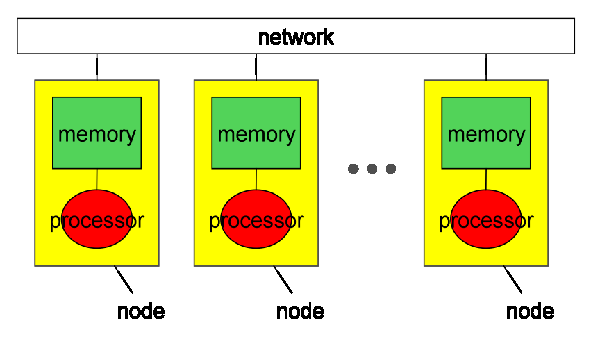
\includegraphics[width=12cm]{figs/Fig1.eps}
  \caption{Target hardware of XMP.}\label{fig1}
\end{figure}


%%%%%%%%%%%%%%%%%%%%%%%%%%%%%%%%%%%%%%%%%%%%%%%%%%%%%%%%%%%%%%%%%%%%%
\subsection{Execution Model}

An {\XMP} program execution is based on the Single Program Multiple Data
(SPMD) model, where each node starts execution from the same main
routine, and continues to execute the same code independently
(i.e., asynchronously), which is referred to as the {\it \Term{replicated
execution}}, until it encounters an {\XMP} construct
(Fig.~\ref{fig:exec_model}).

A set of nodes that executes a procedure, statement, loop,
a block, etc. is referred to as its {\it \Term{executing node set}}, and is
determined by the innermost {\tt task}, {\tt loop}, or {\tt array}
directive surrounding it dynamically, or at runtime.
%
The {\it \Term{current executing node set}} is an executing node set of
the current context, which is managed by the {\XMP} runtime system on
each node.

The current executing node set at the beginning of the program
execution, or {\it \Term{entire node set}}, is a node set that
contains all the available nodes, which can be specified in an 
implementation-defined way (e.g., through a command-line option).

When a node encounters at runtime either a {\tt loop}, {\tt array}, or
{\tt task} construct, and is contained by the node set specified by the
{\tt on} clause of the directive, it updates the current executing node
set with the specified one and executes the body of the construct, after
which it resumes the last executing node set and proceeds to execute the
subsequent statements.

In particular, when a node in the current executing node set encounters a
{\tt loop} or an {\tt array} construct, it executes the loop or the array
assignment in parallel with other nodes, so that each iteration of the
loop or element of the assignment is independently executed by the node
in which a specified data element resides.

When a node encounters a synchronization or a communication directive,
synchronization or communication occurs between it and other nodes.
%
That is, such {\it \Term{global constructs}} are performed collectively
by the current executing nodes.
%
Note that neither synchronization nor communication occurs unless these
constructs are specified.

\begin{figure}
  \centering
  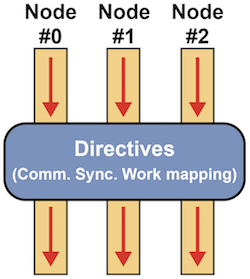
\includegraphics{figs/execution.png}
  \caption{Execution model of XMP.}\label{fig:exec_model}
\end{figure}


%%%%%%%%%%%%%%%%%%%%%%%%%%%%%%%%%%%%%%%%%%%%%%%%%%%%%%%%%%%%%%%%%%%%%
\subsection{Data Model}

There are two classes of data in {\XMP}: {\it \Term{global data}} and
{\it \Term{local data}}. Data declared in an {\XMP} program are local by
default.

Global data are distributed onto the executing node set by
the {\tt align} directive (see section \ref{sub:align}). Each fragment
of distributed global data is allocated in the local memory of a node in the
executing node set.

Local data comprises all data that are not global. They are replicated
within the local memory of each of the executing nodes.

A node can access directly only local data and sections of global data
that reside in its local memory.
%
To access data in remote memory, explicit communication must be
specified in such ways as global communication constructs and
coarray assignments.

In particular, in {\XMPF}, for common blocks that include any global
variables, it is implementation-defined what storage sequences they
occupy and how storage association is defined between two of them.

\begin{figure}
  \centering
  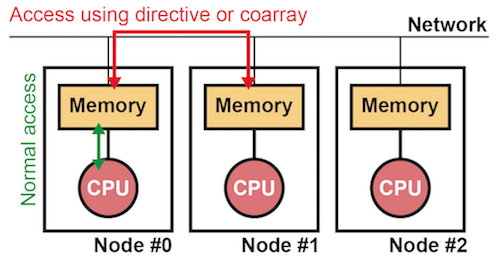
\includegraphics{figs/architecture.png}
  \caption{Data model of XMP.}\label{fig:data_model}
\end{figure}


%%%%%%%%%%%%%%%%%%%%%%%%%%%%%%%%%%%%%%%%%%%%%%%%%%%%%%%%%%%%%%%%%%%%%
\subsection{Programming Models}

\subsubsection{Partitioned Global Address Space}

%Based on the above models that XMP follows, 
XMP can be classified as a
partitioned global address space (PGAS) programming model, such as
Co-Array Fortran~\cite{caf}, Unified Parallel C~\cite{upc}, and
Chapel~\cite{chapel}.

In the PGAS model, multiple executing entities (i.e. threads, processes,
or nodes in XMP) share a part of their address space, which is, however,
partitioned and a portion of which is local to each executing entity.

The two programming models, global-view and local-view, that XMP
supports to achive high performance and productivity on PGAS are
explained below.

\subsubsection{Global-view Programming Model}

The global-view programming model is useful when, starting from a
sequential version of a program, the programmer parallelizes it in
data-parallel style by adding directives with minimum modification.
%
In the global-view programming model, the programmer describes the
distribution of data among nodes using the data distribution
directives.
%
The {\tt loop} construct assigns each iteration of a loop to the node
at which the computed data is located. 
%
The global-view communication directives are used to synchronize nodes,
maintain the consistency of shadow areas, and move sections of 
distributed data globally.
%
Note that the programmer must specify explicitly communications to make
all data references in the program local, and this is done using
appropriate directives.

In many cases, the {\XMP} program according to the global-view
programming model is based on a sequential program, and it can produce
the same results, regardless of the number of nodes (Fig.~\ref{fig2}).

There are three groups of directives for the global-view programming
model. Because these directives are ignored as a comment by the
compilers of base languages ({\Fort} and {\C}), an {\XMP} program can be
compiled by them to ensure that they run properly.

\begin{itemize}
  \item {\it Data mapping,} which specifies the data distribution and mapping
		to nodes (partially inherited from HPF).
  \item {\it Work mapping (parallelization),} which assigns a work to a node
		set. The {\tt loop} construct maps each iteration of a loop to
		nodes owning a specific data elements. The {\tt task} construct
		defines a set amount of work as a {\it \Term{task}}, and assigns
		it to a specific node set.
  \item {\it Communication and synchronization,} which specify how to
		communicate and synchronize with the other compute nodes. In
		{\XMP}, inter-node communication must be explicitly specified by
		the programmer. The compiler guarantees that no communication
		occurs unless it is explicitly specified by the programmer.
\end{itemize}

\begin{figure}
  \centering
  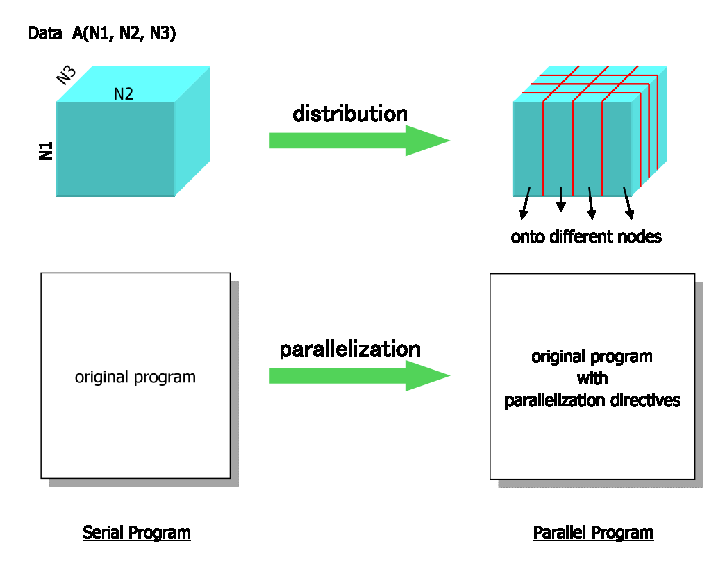
\includegraphics[width=12cm]{figs/Fig2.eps}
  \caption{Parallelization using the global-view programming model.}
\label{fig2}
\end{figure}


\subsubsection{Local-view Programming Model}

The local-view programming model is suitable for programs that
implement an algorithm and a remote data reference that are to
be executed by each node (Fig.~\ref{fig3}).

For the local-view programming model, some language extensions and 
directives are provided. The coarray notation, which is imported from
{\Fort} 2008,
is one such extension, and can be used to specify data on which node 

is to be accessed. For example, the expression of {\tt
A(i)[N]} is used to access an array element of {\tt A(i)} located on the
node {\tt N}.
%
If the access is a reference, then a one-sided communication to read the
value from the remote memory (i.e., the {\it get} operation) is issued
by the executing node.
If the access is a definition, then a one-sided communication to write
the value to the remote memory (i.e., the {\it put} operation) is issued by
the executing node.

\begin{figure}
  \centering
  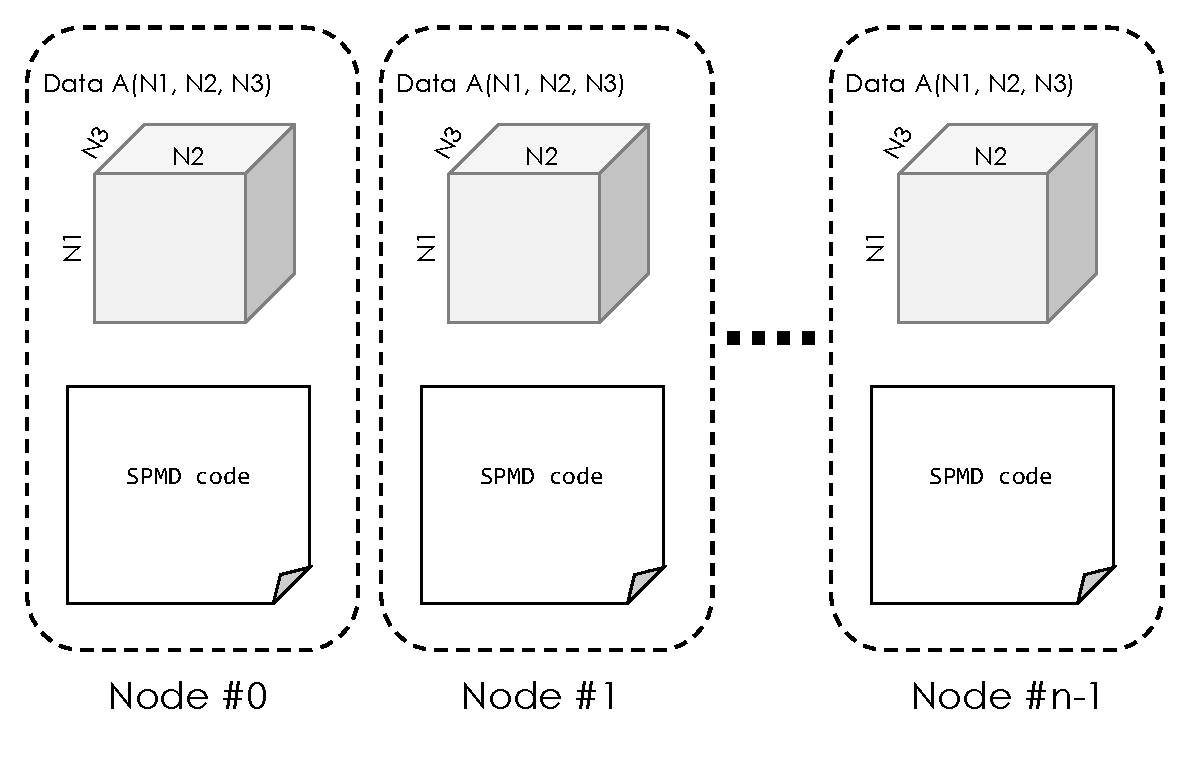
\includegraphics[width=12cm]{figs/Fig3.eps}
  \caption{Local-view programming model.}
\label{fig3}
\end{figure}


\subsubsection{Mixture of Global View and Local View}

In the global-view model, nodes are used to distribute data and works. In the
local-view model, nodes are used to address remote data in the coarray
notation.
%
In application programs,
programmers should choose an appropriate data model according to the
characteristics of their program. Fig.~\ref{fig4} illustrates the global view
and the local view of data.

Data may have both a global view and a local view, and can be accessed
in both of the views. {\XMP} provides a directive to give the local name
(alias) to global data declared in the global-view programming model
to enable them to also be accessed in the local-view programming
model. This feature is useful to optimize a certain part of a program
by using explicit remote data access in the local-view programming
model.

\begin{figure}
  \centering
  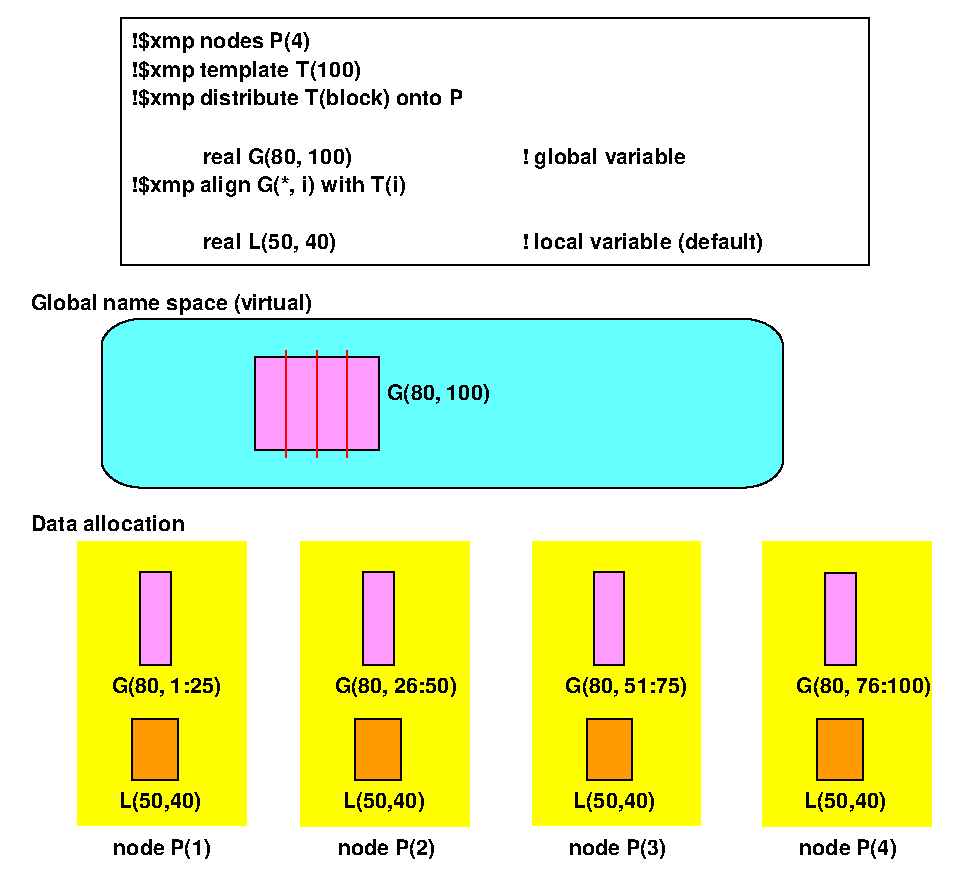
\includegraphics[width=12cm]{figs/Fig4.eps}
  \caption{Global view and local view.}
  \label{fig4}
\end{figure}


\subsection{Base Languages}

The XcalableMP language specification is defined based on Fortran
and C as the base languages. More specifically, the base language of
XcalableMP Fortran is Fortran 90 or later, and that of XcalableMP C is
ISO C90 (ANSI C89) or later with some extensions (see below).

\subsubsection{Array Section in {\XMPC}}

% \label{173437_31Oct14}

% \subsubsection*{Synopsis}

% The array section notation is a notation to describe a part of an array, 
% which is adapted in Fortran.

% \subsubsection*{Syntax}
% \index{array section in XMP/C}
% \index{Syntax!array section in XMP/C}

% \begin{tabular}{llll}
% \verb![C]! & {\it array-section} & {\bf is} & {\it array-name}{\tt [} \{
%  {\it triplet} $\vert$ {\it int-expr} \} {\tt ]}...
% \end{tabular}

% \vspace{0.5cm}

% %where {\it triplet} must be one of:
% where {\it triplet} is:

% \vspace{0.3cm}

% \begin{tabular}{ll}
%  \hspace{0.5cm} & {\openb}{\it base}{\closeb} {\tt :}
%   {\openb}{\it length}{\closeb} {\openb}{\tt :} {\it step}{\closeb}\\
% % \hspace{0.5cm} & {\tt :} \\
% \end{tabular}

% \subsubsection*{Description}

In {\XMPC}, the base language C is extended so that a part of an array,
that is, an {\it array section} or {\it subarray}, can be put in an {\it
array assignment statement}, which is described in \ref{subsubsec:Array
assignment statements in C}, and some {\XMP} constructs.
%
An array section is built from a subset of the elements of an array,
which is specified by a sequence of square-bracketed integer expressions
or {\it triplets}, which are in the form of:

\begin{center}
  [ {\it base} ] {\tt :}
  [ {\it length} ] [ {\tt :} {\it step} ]
\end{center}

When {\it step} is positive, the {\it triplet} specifies a set of
subscripts that is a regularly spaced integer sequence of length {\it
length} beginning with {\it base} and proceeding in increments of {\it
step} up to the largest.
%
The same applies to negative {\it step} too.

When {\it base} is omitted, it is assumed to be 0. When {\it length}
is omitted, it is assumed to be the number of remainder elements of the
dimension of the array. When {\it step} is omitted, it is assumed to be 1.

\subsubsection*{Example}
\index{Example!array section in XMP/C}

Assuming that an array {\tt A} is declared by the following statement,

\vspace{0.3cm}

\begin{tabular}{ll}
\hspace{0.5cm} & {\tt int A[100];} \\
\end{tabular}

\vspace{0.3cm}

\hspace{-0.55cm}some array sections can be specified as follows:

\vspace{0.3cm}

\begin{tabular}{lll}
\hspace{0.5cm} & {\tt A[10:10]} & array section of 10 elements from {\tt
 A[10]} to {\tt A[19]} \\
 & {\tt A[10:]} & array section of 90 elements from
		  {\tt A[10]} to {\tt A[99]}\\
 & {\tt A[:10]} & array section of 10 elements from {\tt A[0]} to {\tt
	 A[9]} \\
 & {\tt A[10:5:2]} & array section of 5 elements from {\tt A[10]} to
	 {\tt A[18]} by step 2 \\
 & {\tt A[:]} & the whole of {\tt A} \\
\end{tabular}


\subsubsection{Array Assignment Statement in {\XMPC}}
\label{subsubsec:Array assignment statements in C}

% \subsubsection*{Synopsis}

% An array assignment statement copies a value into each element of
% an array section.

% \subsubsection*{Syntax}
% \index{array assignment in XMP/C}
% \index{Syntax!array assignment in XMP/C}

% \begin{tabular}{ll}
% \verb![C]! & {\it array-section} {\openb}{\tt :}{\tt [}{\it int-expr}{\tt
%  ]}...{\closeb} {\tt =} {\it expression}{\tt ;}\\
% \end{tabular}

% \subsubsection*{Description}

The value of each element of the result of the right-hand side expression is
assigned to the corresponding element of the array section on the
left-hand side.
%
When an operator or an elemental function (see section
\ref{094142_25Sep13}) is applied to array sections in the right-hand side
expression, it is evaluated to an array section that has the same shape
as that of the operands or arguments, and each element of which is the
result of the operator or function applied to the corresponding element
of the operands or arguments. A scalar object is assumed to be an array
section that has the same shape as that of the array section(s), and
where each element has its value.

Note that an array assignment is a statement, and therefore cannot
appear as an expression in any other statements.

% \subsubsection*{Restrictions}

% \begin{itemize}
%  \item \verb![C]! any array section appearing in the right-hand side expression and
% 	   the left-hand side must have the same shape, i.e., the same number of
% 	   dimensions and size of each dimension.
%  % \item \verb![C]! When the right-hand side is an array section, the left-hand side and the right-hand side
%  %       must have the same shape, i.e., the same number of dimensions and
%  %       size of each dimension.
%  \item \verb![C]! If {\it array-section} on the left-hand side is followed by
%        ``{\tt :}{\tt [}{\it int-expr}{\tt ]}...'', it must be a coarray.
%  % \item \verb![C]! If {\it variable} on the right-hand side is followed by
%  %       ``{\tt :}{\tt [}{\it int-expr}{\tt ]}...'', it must be a coarray.
% \end{itemize}

\subsubsection*{Examples}
\index{Example!array assignment in XMP/C}

An array assignment statement in the fourth line copies the elements
{\tt B[0]} through {\tt B[4]} into the elements {\tt A[5]} through {\tt
A[9]}.

\hspace{\hsize}
\begin{XCexample}
int A[10];
int B[5];
    ...
A[5:5] = B[0:5]; 
\end{XCexample}


% \subsubsection{Built-in Functions for Array Section}
% \index{built-in functions of XMP/C}

% Some built-in functions are defined that can accept one or more array
% sections as arguments. In addition, some of them are array-valued.
% %
% Such array-valued functions can appear in the right-hand side of an
% array assignment statement, and should be preceded by the {\tt array}
% directive if the array section is distributed.

% All of the built-in functions for array sections are described in
% Sections \ref{094142_25Sep13} and \ref{112125_19Sep13}.


% \subsubsection{Pointer to Global Data}
% \label{sec:pointer to global data}

% \paragraph{Name of Global Array}

% The name of a global array is considered to represent an abstract entity
% in the {\XMP} language. It is not interpreted as the pointer to the array,
% while the name of a local array is.

% However, the name of a global array that appears in an expression is
% evaluated to the base address of its local section on each node. The
% pointer can be operated on each node as if it were a normal (local)
% pointer.

% \paragraph{Address-of Operator}
% \index{address-of operator}

% The result of the address-of operator (``{\tt \&}'') applied to an
% element of a global array is the pointer to the corresponding element of
% its local section. Note that the value of the result pointer is defined
% only on the node that owns the element. The pointer can be operated on
% the node as if it were a normal (local) pointer.

% As a result, for a global array {\tt a}, {\tt a} and {\tt \&a[0]} are
% not always evaluated to the same value.

\subsubsection{Support for Intrinsic/Built-in Functions of the Base
	  Languages}

This section describes how intrinsic/built-in functions of the base
languges work on XMP's global arrays.

Many other intrinsic and library procedures, such as mapping inquiry
functions and transformational procedures, are defined in XMP. See the
language specification for their detail.

\paragraph{Array Intrinsic Functions in {\XMPF}}
\index{array intrinsic functions}

The array intrinsic functions of the base language Fortran are
classified into three classes: {\it inquiry}, {\it elemental}, and
{\it transformational}.

It is specified as follows how these functions work in the XMP/F
programs when a global array appears as an argument.

\begin{itemize}
 \item Inquiry functions

       The inquiry functions with a global array or its subobject
       being an argument are regarded as inquiries about the global
       array, and return its ``global'' properties as if it were not
       distributed.

 \item Elemental functions

       The result of the elemental functions with a global array or
       its subobject being an argument has the same shape and
       mapping as the argument.
%
       Note that such a reference of these elemental functions is in
       effect limited to be in the {\tt array} construct.

 \item Transformational functions

       It is unspecified how the transformational functions work when a
       global array or its subobject appears as an argument.
%
       A processor shall detect such a reference of these functions
       and issue a warning message for it.
%
       Some intrinsic transformational subroutines are defined in
       section \ref{112125_19Sep13} as alternatives to these
       transformational functions.

\end{itemize}


\paragraph{Built-in Elemental Functions in {\XMPC}}
\label{094142_25Sep13}
\index{built-in elemental functions}

Some built-in elemental functions that can operate each element of
array arguments are defined in {\XMPC}. Such a built-in function
accepts one or more array sections as its arguments and returns an
array-valued result having the same shape and mapping as the argument.
%
The values of the elements of the result are the same as what would have
been obtained if the scalar function of the C standard library had
been applied separately to the corresponding elements of each array
argument.

These functions may appear on the right-hand side of an array
assignment statement, and it should be preceded by the {\tt array}
directive if the array section is distributed.

Table \ref{tab:elemental_c} shows the list of built-in elemental
functions in {\XMPC}. Their elementwise behavior is the same as those of
the corresponding functions in the C standard library.

\begin{table}[h]
 \caption[Built-in elemental functions in {\XMPC}]{Built-in elemental
 functions in {\XMPC}. (The first line refers to the element type of their
 argument(s) and return value.)}
 \label{tab:elemental_c}
 \begin{center}
 \begin{tabular}{c|c|c} \hline\hline
 double & float & long double \\ \hline
 acos & acosf & acosl \\
 asin & asinf & asinl \\
 atan & atanf & atanl \\
 atan2 & atan2f & atan2l \\
 cos & cosf & cosl \\
 sin & sinf & sinl \\
 tan & tanf & tanl \\

% acosh & acoshf & acoshl \\
% asinh & asinhf & asinhl \\
% atanh & atanhf & atanhl \\
 cosh & coshf & coshl \\
 sinh & sinhf & sinhl \\
 tanh & tanhf & tanhl \\

 exp & expf & expl \\
% exp2 & exp2f & exp2l \\
% expm1 & expm1f & expm1l \\
 frexp & frexpf & frexpl \\
% ilogb & ilogbf & ilogbl \\
 ldexp & ldexpf & ldexpl \\
 log & logf & logl \\
 log10 & log10f & log10l \\
% log1p & log1pf & log1pl \\
% log2 & log2f & log2l \\
% logb & logbf & logbl \\
%% modf & modff & modfl \\
% scalbn & scalbnf & scalbnl \\
% scalbln & scalblnf & scalblnl \\

% cbrt & cbrtf & cbrtl \\
 fabs & fabsf & fabsl \\
% hypot & hypotf & hypotl \\
 pow & powf & powl \\
 sqrt & sqrtf & sqrtl \\

% erf & erff & erfl \\
% erfc & erfcf & erfcl \\
% lgamma & lgammaf & lgammal \\
% tgamma & tgammaf & tgammal \\

 ceil & ceilf & ceill \\
 floor & floorf & floorl \\
% near byint near byintf near byintl \\
% rint & rintf & rintl \\
% lrint & lrintf & lrintl \\
% llrint & llrintf & llrintl \\
% round & roundf & roundl \\
% lround & lroundf & lroundl \\
% llround & llroundf & llroundl \\
% trunc & truncf & truncl \

 fmod & fmodf & fmodl \\ \hline
% remainder & remainderf & remainderl \\
% remquo & remquof & remquol \\
%
% copysign & copysignf & copysignl \\
% nan & nanf & nanl \\
% next after next afterf next afterl \\
% next toward next towardf & next towardl \\
%
% fdim & fdimf & fdiml \\
% fmax & fmaxf & fmaxl \\
% fmin & fminf & fminl \\

% fma & fmaf & fmal \\
 \end{tabular} 
 \end{center}
\end{table}


%%%%%%%%%%%%%%%%%%%%%%%%%%%%%%%%%%%%%%%%%%%%%%%%%%%%%%%%%%%%%%%%%%%%%
\subsection{Interoperability}

Most of existing parallel applications are written with MPI. It is not
realistic to port them over to XMP because each of them consists of
millions of lines.

Because XMP is interoperable with MPI, users can develop an XMP
application by modifying a part of an existing one instead of rewriting
it totally. Besides, when developing a parallel application from
scratch, it is possible to use XMP to write a complicated part of, for
example, domain decomposition while they use MPI, which could be faster
than XMP, to write a hot-spot part that need to be tuned carefully. In
addition, XMP is interoperable with OpenMP and Python (see Chapter
\ref{python}).

It might be difficult to develop an application with just one
programming language or framework since it generally has its own strong
and weak points. Thus, an XMP program is interoperable with those in
other languages to provide both high productivity and performance.
\section{Data Mapping}

\subsection{{\tt nodes} Directive}

The {\tt nodes} directive declares a {\it node array}, which is an
array-like arrangement of {\nodes} in a {\nset}. A {\narray} can be
multi-dimensional.

%\subsubsection{One-dimensional Node Set}

\begin{XCexample}
#pragma xmp nodes p[4]
\end{XCexample}

\begin{XFexample}
!$xmp nodes p(4)
\end{XFexample}

The \|nodes| directive declares a one-dimensional {\narray} \|p| that
includes four nodes. In XMP/C, it is zero-based and consists
of \|p[0]|, \|p[1]|, \|p[2]|, and \|p[3]|. In XMP/Fortran, it is
one-based and consists of \|p(1)|, \|p(2)|, \|p(3)|, and \|p(4)|.

%\subsubsection{Multi-dimensional Node Set}

\begin{XCexample}
#pragma xmp nodes p[2][3]
\end{XCexample}

\begin{XFexample}
!$xmp nodes p(3,2)
\end{XFexample}

The \|nodes| directive declares two-dimensional {\narray} \|p| that
includes six nodes. In XMP/C, it consists of \|p[0][0]|,
\|p[0][1]|, \|p[0][2]|, \|p[1][0]|, \|p[1][1]|, and \|p[1][2]|. In
XMP/Fortran, it consists of \|p(1,1)|, \|p(2,1)|, \|p(3,1)|,
\|p(1,2)|, \|p(2,2)|, and \|p(3,2)|.

\begin{mynote}
  The ordering of the elements in a {\narray} follows that of a normal
  array in the base language, C or Fortran. 
\end{mynote}

%\subsubsection{Dynamic Node Set}

\begin{XCexample}
#pragma xmp nodes p[*]
\end{XCexample}

\begin{XFexample}
!$xmp nodes p(*)
\end{XFexample}

An asterisk can be specified as the size in the \|nodes| directive to declare a
{\it dynamic} {\narray}. In the above code, one-dimensional dynamic
{\narray} \|p| is declared with an asterisk as the size. The actual
size of a dynamic {\narray} is determined at runtime to fit the size of
the current executing node set.
%
For example, when
the programmer runs the sample code with three nodes, the {\narray}
\|p| includes three nodes.

They can also declare multi-dimensional dynamic {\narrays} with an
asterisk.

\begin{XCexample}
#pragma xmp nodes p[*][3]
\end{XCexample}

\begin{XFexample}
!$xmp nodes p(3,*)
\end{XFexample}

When the programmer runs the sample code with 12 nodes, the {\narray} \|p|
has a shape of 4x3, in C, or 3x4, in Fortran.

\begin{mynote}
  The user can put an asterisk only in the last dimension, in
  XMP/Fortran, or the first dimension, in XMP/C of the {\narray}.
\end{mynote}

\begin{myhint}
  The dynamic {\narray} may interfere with compiler optimizations. In
  general, programs with static ones achieve better performance.
\end{myhint}

%\subsubsection{Partial Node Set}

The programmer can declare a node subarray derived from an existing node
array. Node subarrays can be used, for example, to optimize inter-node
communication by reducing the number of nodes participating in the
communication.

\begin{XCexample}
#pragma xmp nodes p[16]
#pragma xmp nodes q[8]=p[0:8]
#pragma xmp nodes r[4][2]=p[8:8]
\end{XCexample}

\begin{XFexample}
!$xmp nodes p(16)
!$xmp nodes q(8)=p(1:8)
!$xmp nodes r(2,4)=p(9:16)
\end{XFexample}

In line 1, a {\narray} \|p| including 16 nodes is declared. In line 2, a
node subarray \|q| corresponding to the first half of \|p| is declared. In line 3, a
two-dimensional node subarray \|r| corresponding to the latter half of \|p| is declared.

The programmer can declare a n-dimensional node subarray derived from a m-dimensional one.

\begin{XCexample}
#pragma xmp nodes p[4][2]
#pragma xmp nodes row[4]=p[:][*]
#pragma xmp nodes col[2]=p[*][:]
\end{XCexample}

\begin{XFexample}
!$xmp nodes p(2,4)
!$xmp nodes row(4)=p(*,:)
!$xmp nodes col(2)=p(:,*)
\end{XFexample}

In line 1, a two-dimensional {\narray} \|p| including 4x2 nodes is
declared. In line 2, a node subarray \|row| derived from a single row of
\|p| is declared. In line 3, a node subarray \|col| derived from a
single column of \|p| is declared.

A colon represents a triplet which indicate all possible indices in the
dimension.
%
An asterisk indicate the index of the current executing node in the
dimension.
%
For example, \|col[2]| corresponds to \|p[0][0:2]| on nodes \|p[0][0]| and
\|p[0][1]|, and to \|p[1][0:2]| on nodes \|p[1][0]| and \|p[1][1]| in
XMP/C. Similarly, \|col(2)| corresponds to \|p(1:2,1)| on nodes
\|p(1,1)| and \|p(2,1)|, and to \|p(1:2,2)| on nodes \|p(1,2)| \|p(2,2)|
in XMP/Fortran.

\begin{figure}
  \centering
  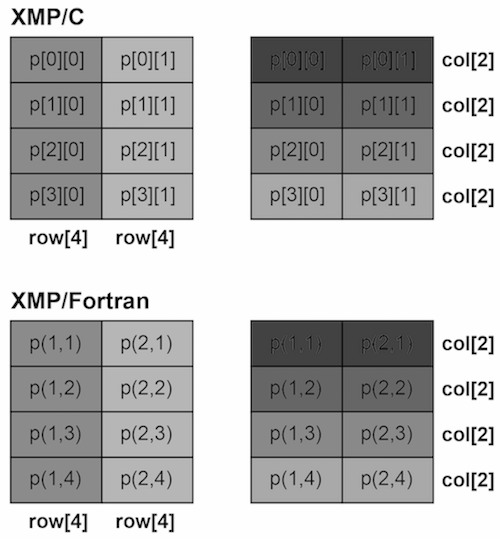
\includegraphics{figs/row_col.png}
  \caption{Node subarrays.}
  \label{fig:partial}
\end{figure}

In XMP/C, \|row[0]| corresponds to \|p[0][0]| and \|p[0][1]| on
\|p[:][0]| and \|p[:][1]|, respectively; 
%
\|col[0]| corresponds to \|p[0][0]|, \|p[1][0]|, \|p[2][0]|, and \|p[3][0]|
on \|p[0][:]|, \|p[1][:]|, \|p[2][:]|, \|p[3][:]|, respectively.
%
In XMP/Fortran, \|row(1)| corresponds to \|p(1,1)| and \|p(2,1)| on
\|p(1,:)| and \|p(2,:)|, respectively;
%
\|col(1)| corresponds to \|p(1,1)|, \|p(1,2)|, \|p(1,3)|, and \|p(1,4)|
on \|p(:,1)|, \|p(:,2)|, \|p(:,3)|, \|p(:,4)|, respectively.

\begin{mynote}
  The semantics of an asterisk in a node reference is different from
  that in a declaraion.
\end{mynote}


\subsection{{\tt template} Directive}

The \|template| directive declares a {\it template}, which is a virtual
array that is used as a ``template'' of parallelization in the programs
and to be distributed onto a {\narray}.
%  Templates are virtual arrays which used for data and work 
% mapping. They can have multi-dimensional shapes.

%\subsubsection{One-dimensional Template}

\begin{XCexample}
#pragma xmp template t[10]
\end{XCexample}

\begin{XFexample}
!$xmp template t(10)
\end{XFexample}

This \|template| directive declares a one-dimensional {\template} \|t|
having ten elements.
%
{\bf Templates} are indexed in the similar manner to
arrays in the base languages. For the above examples, the {\template} \|t|
is indexed from zero to nine (i.e. \|t[0]| $\cdots$ \|t[9]|), in XMP/C,
or one to ten (i.e. \|t(1)| $\cdots$ \|t(10)|), in XMP/Fortran.

\begin{myhint}
% In general, the user declare templates which has the same
% size with the target data array.
  In many cases, a template should be declared to have the same shape as
  your target array.
\end{myhint}

% In XMP/Fortran, the start index of the template can be given by an
% arbitrary number to match the starting array index in the base
% language.

% \begin{XFexample}
% !$xmp template t(-5:4)
% \end{XFexample}

% The template directive declares 1-dimensional template t starting from t(-5) to t(4).

% \begin{mynote}
% In XMP/C, templates should start from 0 since array indices
% start from 0 in the C language.
% \end{mynote}

%\subsubsection{Multi-dimensional Template}

\begin{XCexample}
#pragma xmp template t[10][20]
\end{XCexample}

\begin{XFexample}
!$xmp template t(20,10)
\end{XFexample}

The \|template| directive declares a two-dimensional {\template} \|t| that
has 10x20 elements. In XMP/C, \|t| is indexed from t[0][0] to t[9][19],
and,  in XMP/Fortran, from \|t(1,1)| to \|t(20,10)|.

%\subsubsection{Dynamic Template}

\begin{XCexample}
#pragma xmp template t[:]
\end{XCexample}

\begin{XFexample}
!$xmp template t(:)
\end{XFexample}

In the above examples, a colon instead of an integer is specified as the
size to declare a one-dimensional dynamic {\template} \|t|. The colon
indicates that the size of the {\template} is not fixed and to be
fixed at runtime by the \|template_fix| construct (Sec. \ref{184243_1Nov19}).


\subsection{{\tt distribute} Directive}

The \|distribute| directive specifies a distribution of the target
{\template}.
%
Either of {\it block}, {\it cyclic}, {\it block-cyclic}, or {\it gblock}
(i.e. uneven block) can be specified to distribute a dimension of a {\template}.


\subsubsection{Block Distribution}

\begin{XCexample}
#pragma xmp distribute t[block] onto p
\end{XCexample}

\begin{XFexample}
!$xmp distribute t(block) onto p
\end{XFexample}

The target template \|t| is divided into contiguous blocks and
distributed among nodes in the {\narray} \|p|.
%
% When the size of the template is $N$ and the
% number of nodes is $K$, the size of each block will be $ceil(N/K)$.
Let's suppose that the size of the {\template} is $N$ and the
number of nodes is $K$. If $N$ is divisible by $K$, a block of size $N/K$
are assigned to each node; otherwise, a block of size
$ceil(N/K)$ is assigned to each of $N/ceil(N/K)$ nodes, a block of size
$mod(N,K)$ to one node, and no block to $(K-N/ceil(N/K)-1)$ nodes. 
%
The block distribution is useful for regular computations such as a
stencil one.

\begin{mynote}
  The function $ceil(x)$ returns a minimum integer value greater than
  $x$, and $mod(x,y)$ returns $x$ modulo $y$.
\end{mynote}

\begin{XCexample}
#pragma xmp nodes p[3]
#pragma xmp template t[22]
#pragma xmp distribute t[block] onto p
\end{XCexample}

\begin{XFexample}
!$xmp nodes p(3)
!$xmp template t(22)
!$xmp distribute t(block) onto p
\end{XFexample}

\begin{figure}
  \centering
  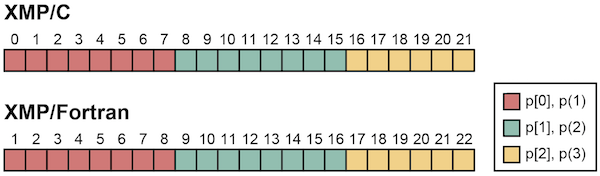
\includegraphics{figs/block.png}
  \caption{Block distribution.}
\end{figure}

Since $ceil(22/3)$ is 8, eight elements are allocated on each of \|p[0]|
and p[1], and the remaining six elements are allocated on \|p[2]|.

% The user can explicitly specify the block size.
% In that case, the remaining elements are allocated on the last node.

% \begin{XCexample}
% #pragma xmp nodes p[3]
% #pragma xmp template t[22]
% #pragma xmp distribute t[block(7)] onto p
% \end{XCexample}

% \begin{XFexample}
% !$xmp nodes p(3)
% !$xmp template t(22)
% !$xmp distribute t(block(7)) onto p
% \end{XFexample}

% \begin{figure}
%   \centering
%   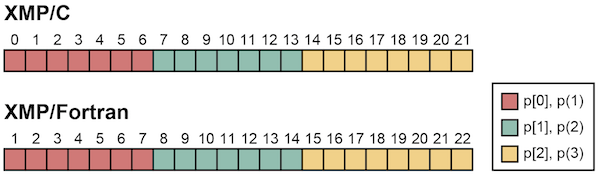
\includegraphics{figs/block2.png}
% \end{figure}

% Seven elements will be allocated on the p[0] and p[1], as specified in
% the directive. And then remaining 8 elements will be allocated on the
% last node p[2].


\subsubsection{Cyclic Distribution}

\begin{XCexample}
#pragma xmp distribute t[cyclic] onto p
\end{XCexample}

\begin{XFexample}
!$xmp distribute t(cyclic) onto p
\end{XFexample}

The target {\template} \|t| is divided into chunks of size one and
distributed among nodes in the {\narray} \|p| in a round-robin manner.
%
The cyclic distribution is usefull for the case where the load on each
element of the {\template} is not balanced.
%suitable for computation with an irregular
%load%balance of data and computation.

\begin{XCexample}
#pragma xmp nodes p[3]
#pragma xmp template t[22]
#pragma xmp distribute t[cyclic] onto p
\end{XCexample}

\begin{XFexample}
!$xmp nodes p(3)
!$xmp template t(22)
!$xmp distribute t(cyclic) onto p
\end{XFexample}

\begin{figure}
  \centering
  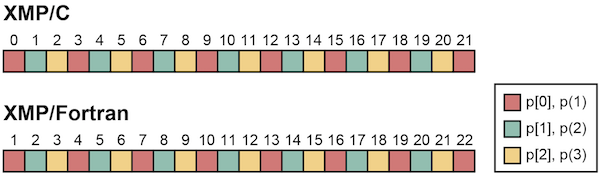
\includegraphics{figs/cyclic.png}
  \caption{Cyclic distribution.}
\end{figure}


\subsubsection{Block-cyclic Distribution}

\begin{XCexample}
#pragma xmp distribute t[cyclic(w)] onto p
\end{XCexample}

\begin{XFexample}
!$xmp distribute t(cyclic(w)) onto p
\end{XFexample}

The target {\template} \|t| is divided into chunks of size \|w| and distributed
among nodes in the {\narray} \|p| in a round-robin manner.
%
The block-cyclic distribution is usefull for the case where the load on
each element of the {\template} is not balanced but the locality of the
elements is required.

% Block-cyclic distribution is
% suitable for computation which has an irregular load balance and
% references to neighborhood elements.

\begin{XCexample}
#pragma xmp nodes p[3]
#pragma xmp template t[22]
#pragma xmp distribute t[cyclic(3)] onto p
\end{XCexample}

\begin{XFexample}
!$xmp nodes p(3)
!$xmp template t(22)
!$xmp distribute t(cyclic(3)) onto p
\end{XFexample}

\begin{figure}
  \centering
  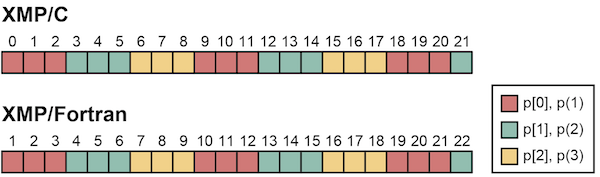
\includegraphics{figs/block-cyclic.png}
  \caption{Block-cyclic distribution.}
\end{figure}


\subsubsection{Gblock Distribution}

\begin{XCexample}
#pragma xmp distribute t[gblock(W)] onto p
\end{XCexample}

\begin{XFexample}
!$xmp distribute t(gblock(W)) onto p
\end{XFexample}

The target {\template} \|t| is divided into contiguous blocks of size \|W[0]|,
\|W[1]|, $\cdots$, in XMP/C, or \|W(1)|, \|W(2)|, $\cdots$, in
XMP/Fortran, and distributed among nodes in the {\narray} \|p|.
%
The array \|W| is called a mapping array.
%
The programmer can specify irregular (uneven) block distribution with
the gblock format.
%a special type of data distribution explicitly by using
%mapping arrays (e.g. distribution of triangular matrix).

\begin{XCexample}
#pragma xmp nodes p[3]
#pragma xmp template t[22]
int W[3] = {6, 11, 5};
#pragma xmp distribute t[gblock(W)] onto p
\end{XCexample}

\begin{XFexample}
!$xmp nodes p(3)
!$xmp template t(22)
integer, parameter :: W(3) = (/6,11,5/)
!$xmp distribute t(gblock(W)) onto p
\end{XFexample}

\begin{figure}
  \centering
  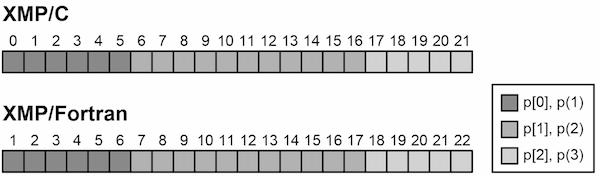
\includegraphics{figs/gblock.png}
  \caption{Gblock distribution.}
\end{figure}

The programmer can specify an asterisk instead of a mapping array in the 
gblock distribution to defer fixing the actual distribution.
%
In such a case, the actual distribution will be fixed at runtime by 
using {\tt template\_fix} construct.


\subsubsection{Distribution of Multi-dimensional Templates}

The programmer can distribute a multi-dimensional {\template} onto
a {\narray}.

\begin{XCexample}
#pragma xmp nodes p[2][2]
#pragma xmp template t[10][10]
#pragma xmp distribute t[block][block] onto p
\end{XCexample}

\begin{XFexample}
!$xmp nodes p(2,2)
!$xmp template t(10,10)
!$xmp distribute t(block,block) onto p
\end{XFexample}

The \|distribute| directive declares the distribution of a two-dimensional
{\template} \|t| onto a two-dimensional {\narray} \|p|. Each dimension of the
{\template} is divided in a block manner and each of the rectangular
regtion is assigned to a node.

\begin{figure}
  \centering
  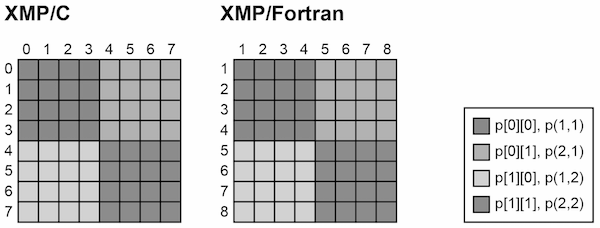
\includegraphics{figs/multi.png}
  \caption{Example of multi-dimensional distribution (1).}
\end{figure}

The programmer can specify a different distribution format in each of
the dimension of a {\template}.

\begin{XCexample}
#pragma xmp nodes p[2][2]
#pragma xmp template t[10][10]
#pragma xmp distribute t[block][cyclic] onto p
\end{XCexample}

\begin{XFexample}
!$xmp nodes p(2,2)
!$xmp template t(10,10)
!$xmp distribute t(cyclic,block) onto p
\end{XFexample}

\begin{figure}
  \centering
  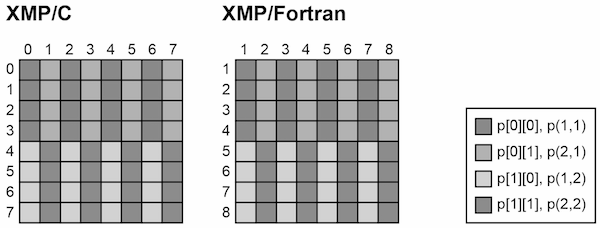
\includegraphics{figs/multi2.png}
  \caption{Example of multi-dimensional distribution (2).}
\end{figure}

When an asterisk is specified in a \|distribute| directive as
a distribution format, the target dimension is ``non-distributed.'' In
the following example, the first dimension is distributed in a
block manner and the second dimension is non-distributed.

\begin{XCexample}
#pragma xmp nodes p[4]
#pragma xmp template t[10][10]
#pragma xmp distribute t[block][*] onto p
\end{XCexample}

\begin{XFexample}
!$xmp nodes p(4)
!$xmp template t(10,10)
!$xmp distribute t(*,block) onto p
\end{XFexample}

\begin{figure}
  \centering
  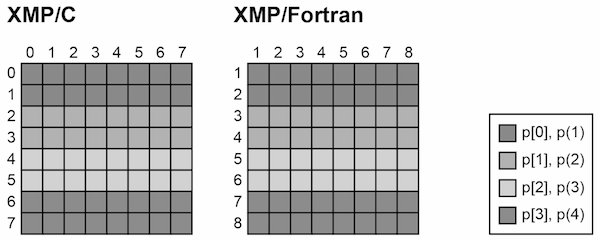
\includegraphics{figs/multi3.png}
  \caption{Example of multi-dimensional distribution (3).}
\end{figure}


\subsection{{\tt align} Directive}

% The {\tt align} directive performs data mapping and distributes data
% among nodes by using a distributed template. The {\tt align} directive
% must follow the definition of the target template.

The \|align| directive specifies that an array is to be mapped in the
same way as a specified {\template}. In other words, an \|align| directive
defines the correspondece of elements between an array and a {\template},
and each of the array element is allocated on the node where the
corresponding {\template} element is allocated.
% As a result of this directive, an array is ``distributed'' onto nodes.

%\subsubsection{Normal Alignment}

\begin{XCexample}
#pragma xmp nodes p[4]
#pragma xmp template t[8]
#pragma xmp distribute t[block] onto p
int a[8];
#pragma xmp align a[i] with t[i]
\end{XCexample}

\begin{XFexample}
!$xmp nodes p(4)
!$xmp template t(8)
!$xmp distribute t(block) onto p
integer :: a(8)
!$xmp align a(i) with t(i)
\end{XFexample}

The array \|a| is decomposed and laid out so that each element
\|a(i)| is colocated with the corresponding {\template} element \|t(i)|.

% The {\tt align} directive aligns the owner node of a[i] with t(i), a
% distributed template. As a result, array a is distributed among the node
% set p.

\begin{figure}
  \centering
  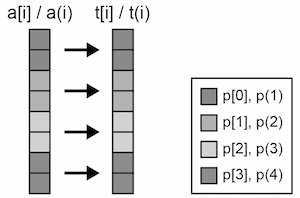
\includegraphics{figs/1dim.png}
  \caption{Example of array alignment (1).}
\end{figure}

The \|align| directive can also be used for multi-dimensional arrays.

\begin{XCexample}
#pragma xmp nodes p[2][2]
#pragma xmp template t[8][8]
#pragma xmp distribute t[block][block] onto p
int a[8][8];
#pragma xmp align a[i][j] with t[i][j]
\end{XCexample}

\begin{XFexample}
!$xmp nodes p(2,2)
!$xmp template t(8,8)
!$xmp distribute t(block,block) onto p
integer :: a(8,8)
!$xmp align a(j,i) with t(j,i)
\end{XFexample}

\begin{figure}
  \centering
  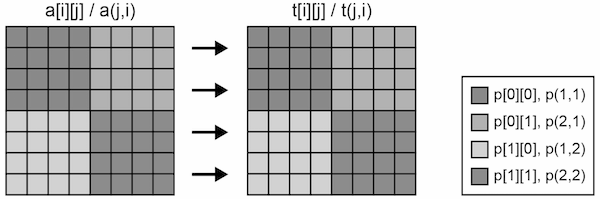
\includegraphics{figs/multi-dim.png}
  \caption{Example of array alignment (2).}
\end{figure}

%\subsubsection{Special Alignment}

%\paragraph{Collapse}

The programmer can align an $n$-dimensional array with an $m$-dimensional
{\template} for $n > m$.

\begin{XCexample}
#pragma xmp nodes p[4]
#pragma xmp template t[8]
#pragma xmp distribute t[block] onto p
int a[8][8];
#pragma xmp align a[i][*] with t[i]
\end{XCexample}

\begin{XFexample}
!$xmp nodes p(4)
!$xmp template t(8)
!$xmp distribute t(block) onto p
integer :: a(8,8)
!$xmp align a(*,i) with t(i)
\end{XFexample}

When an asterisk is specified as a subscript in a dimension of the
target array in the \|align| directive, the dimension is ``collapsed''
(i.e. not distributed). In the sample program above, the first dimension of the
array {\tt a} is distributed onto the {\narray} \|p| while the second
dimension is collapsed.

\begin{figure}
  \centering
  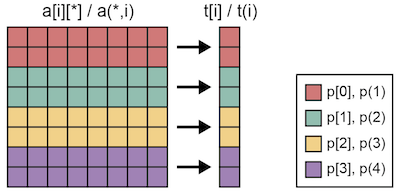
\includegraphics{figs/collapse.png}
  \caption{Example of array alignment (3).}
\end{figure}

In XMP/C, {\tt a[0:2][:]} will be allocated on {\tt p[0]} while, in
XMP/Fortran, \|a(:,1:2)| will be allocated on \|p(1)|.

%\paragraph{Replicate}

The programmer also can align an $n$-dimensional array with an
$m$-dimensional template for $n < m$.

\begin{XCexample}
#pragma xmp nodes p[2][2]
#pragma xmp template t[8][8]
#pragma xmp distribute t[block][block] onto p
int a[8];
#pragma xmp align a[i] with t[i][*]
\end{XCexample}

\begin{XFexample}
!$xmp nodes p(2,2)
!$xmp template t(8,8)
!$xmp distribute t(block,block) onto p
integer :: a(8)
!$xmp align a(i) with t(*,i)
\end{XFexample}

When an asterisk is specified as a subscript in a dimension of the
target {\template} in the \|align| directive, the array will be
``replicated'' along the axis of the dimension.

\begin{figure}
  \centering
  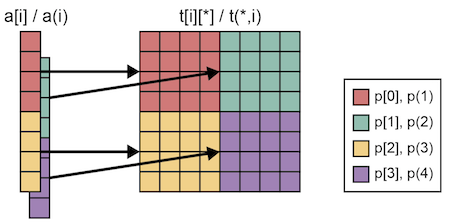
\includegraphics{figs/replicate.png}
  \caption{Example of array alignment (4).}
\end{figure}

In XMP/C, \|a[0:4]| will be replicated and allocated on p[0][0] and
p[0][1] while, in XMP/Fortran, \|a(1:4)| will be allocated on \|p(1,1)|
and \|p(2,1)|.


\subsection{Dynamic Allocation of Distributed Array}

This section explains how {\bf distributed} (i.e. {\bf global}) {\bf
arrays} are allocated 
at runtime. The basic procedure is common in XMP/C and XMP/Fortran with
a few specific difference.

%\subsubsection{One-dimensional Array}

\begin{XCexample}
#pragma xmp nodes p[4]
#pragma xmp template t[N]
#pragma xmp distribute t[block] onto p
float *a;
#pragma xmp align a[i] with t[i]
  :
a = xmp_malloc(xmp_desc_of(a), N);
\end{XCexample}

In XMP/C, first, declare a pointer of the type of the target array; 
%
second, align it as if it were an array;
%
finally, allocate memory for it with the {\tt xmp\_malloc()}
function. {\tt xmp\_desc\_of()} is an 
intrinsic/builtin function that returns the descriptor of the XMP object
(i.e. {\nodes}, {\templates}, or {\garrays}) specified by the argument.

\begin{XFexample}
!$xmp nodes p(4)
!$xmp template t(N)
!$xmp distribute t(block) onto p
real, allocatable :: a(:)
!$xmp align a(i) with t(i)

allocate(a(N))
\end{XFexample}

In XMP/Fortran, first, declare an allocatable array; second, align it;
finally, allocate memory for it with the \|allocate| statement.

%\subsubsection{Multi-dimensional Array}

For multi-dimensional arrays, the procedure is the same as that for 
one-dimensional ones, as follows:

\begin{XCexample}
#pragma xmp nodes p[2][2]
#pragma xmp template t[N1][N2]
#pragma xmp distribute t[block][block] onto p
float (*a)[N2];
#pragma xmp align a[i][j] with t[i][j]
  :
a = (float (*)[N2])xmp_malloc(xmp_desc_of(a), N1, N2);
\end{XCexample}

\begin{XFexample}
!$xmp nodes p(2,2)
!$xmp template t(N2,N1)
!$xmp distribute t(block,block) onto p
real, allocatable :: a(:,:)
!$xmp align a(j,i) with t(j,i)
  :
allocate(a(N2,N1))
\end{XFexample}

\begin{mynote}
  If the size of the {\template} is not fixed until runtime, the programmer
  have to fixe it at runtime with the \|template_fix| construct.
\end{mynote}


\subsection{{\tt template\_fix} Construct}
\label{184243_1Nov19}

The \|template_fix| construct fixes the shape and/or the distribution of
an unfixed {\template}. 
%It is also used when a distributed array is allocated at runtime.

\begin{XCexample}
#pragma xmp nodes p[4]
#pragma xmp template t[:]
#pragma xmp distribute t[block] onto p
double *a;
#pragma xmp align a[i] with t[i]

int n = 100;
#pragma xmp template_fix t[n]
a = xmp_malloc(xmp_desc_of(a), n);
\end{XCexample}

\begin{XFexample}
!$xmp nodes p(4)
!$xmp template t(:)
!$xmp distribute t(block) onto p
real, allocatable :: a(:)
integer :: n
!$xmp align a(i) with t(i)

n = 100
!$xmp template_fix t(n)
allocate(a(n))
\end{XFexample}

In the above sample code, 
%
first, a {\template} \|t| whose size is unfixed (``\|:|'') is declared;
%
second, a pointer \|a|, in XMP/C, or an allocatable array \|a|, in
XMP/Fortran, is aligned with the {\template};
%
third, the size of the {\template} is fixed with a \|template_fix|
construct;
%
finally, the pointer or the allocatable array is allocated with the
\|xmp_malloc()| builtin function in XMP/C or the \|allocate| statement
in XMP/Fortran, respectively.

\begin{mynote}
The {\tt template\_fix} constructs can be applied to a {\template} only once.
\end{mynote}

This construct can also be used to fix a mapping array of a {\template}
that is distributed in ``\|gblock(*)|`` at declaration.

\begin{XCexample}
#pragma xmp nodes p[4]
#pragma xmp template t[:]
#pragma xmp distribute t[gblock(*)] onto p
double *a;
#pragma xmp align a[i] with t[i]

int n = 100;
int m[] = {40,30,20,10};

#pragma xmp template_fix[gblock(m)] t[n]
a = xmp_malloc(xmp_desc_of(a), n);
\end{XCexample}

\begin{XFexample}
!$xmp nodes p(4)
!$xmp template t(:)
!$xmp distribute t(gblock) onto p
real, allocatable :: a(:)
integer :: n, m(4)
!$xmp align a(i) with t(i)

n = 100
m(:) = (/40,30,20,10/)
!$xmp template_fix(gblock(m)) t(n)
allocate(a(n))
\end{XFexample}

\section{Work Mapping}

\subsection{{\tt task} and {\tt tasks} Construct}

The \|task| construct defines a {\it task} that is executed by a specified
{\nset}. The \|tasks| construct asserts that surrounding \|task|
constructs can be executed in parallel.

% This page shows some examples of the task construct other than those in
% Tutorial (Global-view).

\subsubsection{{\tt task} Construct}

When a {\node} encounters a {\it task} construct at runtime, it executes
the associated block (called a task) if it is included by the {\nset}
specified by the \|on| clause; otherwise, it skips the execution of the
block.

% The \|on| clause of the \|task| construct specifies the node set that
% executes the task.

\begin{XCexample}
#include <stdio.h>
#pragma xmp nodes p[4]

int main(){
  int num = xmpc_node_num();
#pragma xmp task on p[1:3]
{
  printf("%d: Hello\n", num);
}

  return 0;
}
\end{XCexample}

\begin{XFexample}
program main
!$xmp nodes p(4)
  integer :: num

  num = xmp_node_num()
!$xmp task on p(2:4)
  write(*,*) num, ": Hello"
!$xmp end task

end program main
\end{XFexample}

In the above example, {\nodes} \|p[1]|, \|p[2]|, and \|p[3]| invokes the \|printf()|
function, and \|p[1]| outputs ``1: Hello'' in XMP/C; \|p(2)|, \|p(3)|, and \|p(4)|
execute the \|write| statement, and \|p(2)| outputs ``2: Hello'' in
XMP/Fortran.

Note that a new {\nset} is generated by each \|task| construct. Let's
consider inserting a \|bcast| construct into the task.

\begin{XCexample}
#pragma xmp task on p[1:3]
{
#pragma xmp bcast (num)
}
\end{XCexample}

\begin{XFexample}
!$xmp task on p(2:4)
!$xmp bcast (num)
!$xmp end task
\end{XFexample}

This \|bcast| construct is executed by the {\nset} specified by the
\|on| clause of the \|task| construct. Thus, the {\node} \|p[1]| broadcasts
the value of \|num| to \|p[2]| and \|p[3]| in XMP/C, and \|p(2)| to
\|p(3)| and \|p(4)| in XMP/Fortran.

\begin{figure}
  \centering
  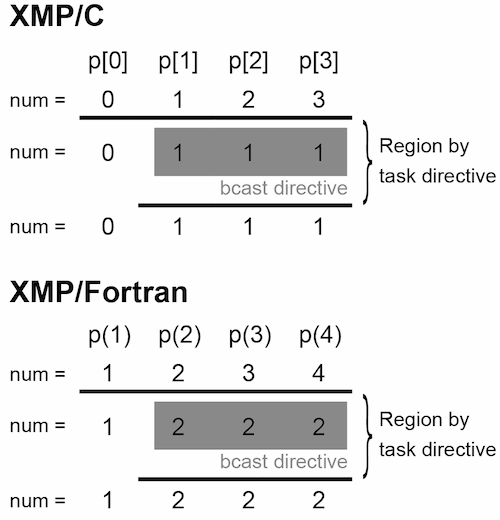
\includegraphics{figs/task.png}
  \caption{Example of {\tt task} construct (1).}
\end{figure}

The \|bcast| construct in the above code is equivalent to that in the
following code, where it is executed by a new {\nset} \|q| that is
explicitly declared.

\begin{XCexample}
#pragma xmp nodes q[3] = p[1:3]
#pragma xmp bcast (num) on q
\end{XCexample}

\begin{XFexample}
!$xmp nodes q(3) = p(2:4)
!$xmp bcast (num) on q
\end{XFexample}

Note that the task is executed by the {\nset} specified by the \|on|
clause. Therefore, {\tt xmpc\_node\_num()} and {\tt xmp\_node\_num()}
return the id in the {\nset}.

For example, consider inserting {\tt xmpc\_node\_num()} or {\tt
xmp\_node\_num()} into the task in the first program.

\begin{XCexample}
#include <stdio.h>
#pragma xmp nodes p[4]

int main(){
#pragma xmp task on p[1:3]
{
  printf("%d: Hello\n", xmpc_node_num());
}

  return 0;
}
\end{XCexample}

\begin{XFexample}
program main
!$xmp nodes p(4)

!$xmp task on p(2:4)
  write(*,*) xmp_node_num(), ": Hello"
!$xmp end task

end program main
\end{XFexample}

The {\node} \|p[1]| outputs ``0: Hello'' in XMP/C, and p(2) ``1: Hello'' in XMP/Fortran.

\begin{mynote}
  A new {\nset} should be collectively generated by all of the executing 
  {\nodes} at the point of a \|task| construct unless it is surrounded by a
  \|tasks| construct. Therefore, in the above example, \|p[0]| in XMP/C
  and \|p(1)| in XMP/Fortran must execute the \|task| construct.
\end{mynote}


\subsubsection{{\tt tasks} Construct}

Let's consider that each of two tasks invokes a function.

\begin{XCexample}
#pragma xmp nodes p[4]

#pragma xmp task on p[0:2]
{
  func_a();
}
#pragma xmp task on p[2:2]
{
  func_b();
}
\end{XCexample}

\begin{XFexample}
!$xmp nodes p(4)

!$xmp task on p(1:2)
  call func_a()
!$xmp end task
!$xmp task on p(3:4)
  call func_b()
!$xmp end task
\end{XFexample}

In the above example, the two tasks cannot be executed in parallel
because those \|on| clauses must be evaluated by all of the {\bf
executing nodes}.

\begin{figure}
  \centering
  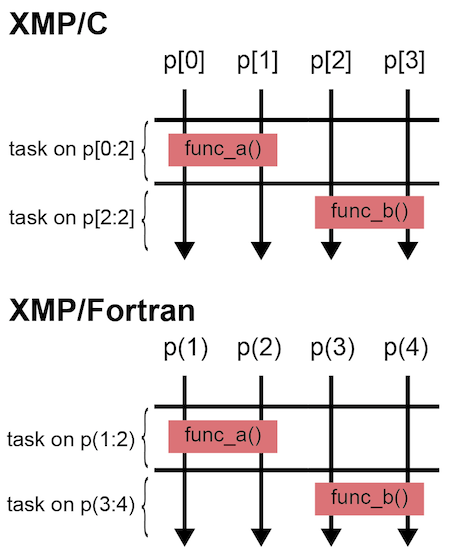
\includegraphics{figs/task_noparallel.png}
  \caption{Example of {\tt task} construct (2).}
\end{figure}

In such a case, the programmer must specify a \|tasks| construct
surrounding the tasks is needed to execute them in parallel.

\begin{XCexample}
#pragma xmp nodes p[4]

#pragma xmp tasks
{
#pragma xmp task on p[0:2]
{
  func_a();
}
#pragma xmp task on p[2:2]
{
  func_b();
}
}
\end{XCexample}

\begin{XFexample}
!$xmp nodes p(4)

!$xmp tasks
!$xmp task on p(1:2)
  call func_a()
!$xmp end task
!$xmp task on p(3:4)
  call func_b()
!$xmp end task
!$xmp end tasks
\end{XFexample}

Because the {\nset}s specified by the \|on| clauses of the \|task|
constructs surrounded by a \|tasks| construct are disjoint, they can be
executed in parallel.

\begin{figure}
  \centering
  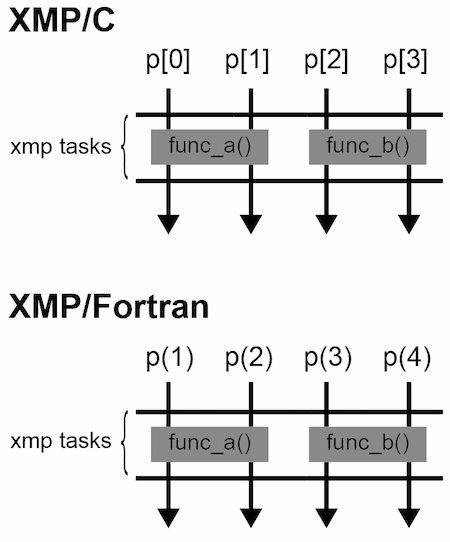
\includegraphics{figs/tasks.png}
  \caption{Example of {\tt tasks} construct.}
\end{figure}


%%%%%%%%%%%%%%%%%%%%%%%%%%%%%%%%%%%%%%%%%%%%%%%%%%%%%%%%%%%%%%%%%%%
\subsection{{\tt loop} Construct}

The \|loop| construct is used to parallelize a loop.

\begin{XCexample}
#pragma xmp loop on t[i]
  for (int i = 0; i < 10; i++)
    a[i] = i;
\end{XCexample}

\begin{XFexample}
!$xmp loop on t(i)
  do i = 1, 10
    a(i) = i
  end do
\end{XFexample}

The \|loop| directive above specifies that the iteration \|i| of the
following loop is executed by the {\node} that owns the {\template} element
\|t[i]| or \|t(i)|, which is specified in the \|on| clause.

Such a loop must satisfy the following two conditions:

\begin{enumerate}
  \item There is no data/control dependence among the iterations. In other
		words, the iterations of the loop can be executed in any order to
		produce the same result.
  \item Elements of {\darrays}, if any, are accessed only by the
		{bf node(s)} that own(s) the elements.
\end{enumerate}

%\subsubsection{Accessing Distributed Arrays in a \|loop| construct}

The programs below are examples of a right \|loop| directive and a loop
statement.
%
The condition 1 is satisfied because \|i| is the only one index
of the {\darray} \|a| that is accessed within the loop,
%
and the condition 2 is also satisfied because the indices of the
{\template} in the \|on| clause of the \|loop| directive is identical to that
of the {\darray}.

\begin{XCexample}
#pragma xmp nodes p[2]
#pragma xmp template t[10]
#pragma xmp distribute t[block] onto p

int main(){
  int a[10];
#pragma xmp align a[i] with t[i]

#pragma xmp loop on t[i]
  for(int i=0;i<10;i++)
    a[i] = i;

  return 0;
}
\end{XCexample}

\begin{XFexample}
program main
!$xmp nodes p(2)
!$xmp template t(10)
!$xmp distribute t(block) onto p
  integer a(10)
!$xmp align a(i) with t(i)

!$xmp loop on t(i)
  do i=1, 10
    a(i) = i
  enddo

end program main
\end{XFexample}

\begin{figure}
  \centering
  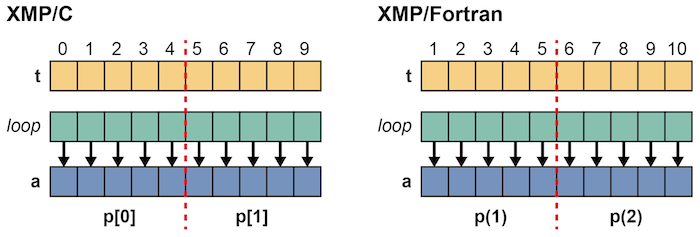
\includegraphics[width=\textwidth]{figs/loop1.png}
  \caption{Example of {\tt loop} construct (1).}
\end{figure}

Then, is it possible to parallelize the loops in the below example where
the loop bounds are shrunk from the above?

\begin{XCexample}
#pragma xmp loop on t[i]
  for(int i=1;i<9;i++)
    a[i] = i;
\end{XCexample}

\begin{XFexample}
!$xmp loop on t(i)
  do i=2, 9
    a(i) = i
  enddo
\end{XFexample}

In this case, the conditions 1 and 2 are satisfied and therefore it is
possible to parallelize them. In XMP/C, \|p[0]| processes the indices from
one to four and \|p[1]| from five to eight. In XMP/Fortran, \|p(1)| processes
the indices from two to five and \|p(2)| from six to nine.

\begin{figure}
  \centering
  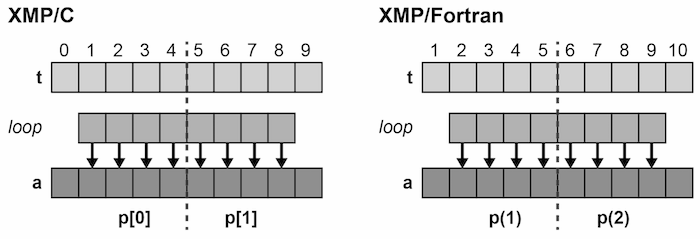
\includegraphics[width=\textwidth]{figs/loop2.png}
  \caption{Example of {\tt loop} construct (2).}
\end{figure}

Next, is it possible to parallelize the below loops in which the index
of the {\darray} is different?

\begin{XCexample}
#pragma xmp loop on t[i]
  for(int i=1;i<9;i++)
    a[i+1] = i;
\end{XCexample}

\begin{XFexample}
!$xmp loop on t(i)
  do i=2, 9
    a(i+1) = i
  enddo
\end{XFexample}

In this case, the condition 1 is satisfied but 2 is not, and therefore
it is not possible to parallelize them. In XMP/C, \|p[0]| tries to access
\|a[5]| but does not own it. In XMP/Fortran, \|p(1)| tries to access
\|a(6)| but does not own it.

\begin{figure}
  \centering
  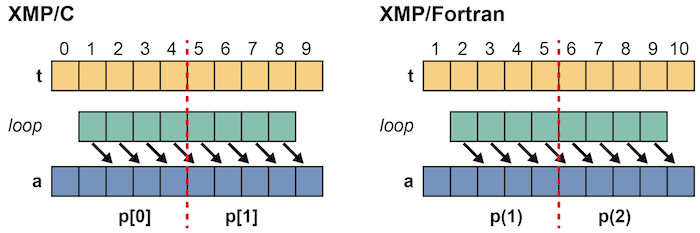
\includegraphics[width=\textwidth]{figs/loop3.png}
  \caption{Example of {\tt loop} construct (3).}
\end{figure}


\subsubsection{Reduction Computation}

The serial programs below are examples of a reduction computation.

\begin{Cexample}
#include <stdio.h>

int main(){
  int a[10], sum = 0;

  for(int i=0;i<10;i++){
    a[i] = i+1;
    sum += a[i];
  }

  printf("%d\n", sum);

  return 0;
}
\end{Cexample}

\begin{Fexample}
program main
  integer :: a(10), sum = 0

  do i=1, 10
    a(i) = i
    sum = sum + a(i)
  enddo

  write(*,*) sum

end program main
\end{Fexample}

If the above loops are parallelized just by adding a \|loop| directive, the
value of the variable \|sum| varies from {\node} to {\node} because it is
calculated separately on each {\node}. The value should be {\it reduced}
to produce the right result.

\begin{XCexample}
#pragma xmp loop on t[i]
   for(int i=0;i<10;i++){
     a[i] = i+1;
     sum += a[i];
   }
\end{XCexample}

\begin{XFexample}
!$xmp loop on t(i)
  do i=1, 10
    a(i) = i
    sum = sum + a(i)
  enddo
\end{XFexample}

\begin{figure}
  \centering
  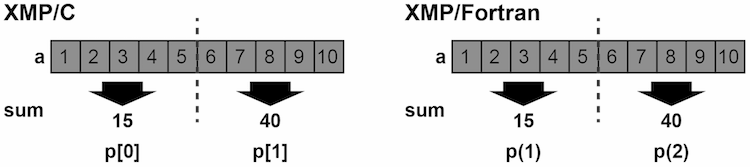
\includegraphics[width=\textwidth]{figs/reduction1.png}
  \caption{Example of reduction computation (1).}
\end{figure}

Then, to correct the error in the above code, add a \|reduction| clause
to the \|loop| directive as follows.

\begin{XCexample}
#include <stdio.h>
#pragma xmp nodes p[2]
#pragma xmp template t[10]
#pragma xmp distribute t[block] onto p

int main(){
  int a[10], sum = 0;
#pragma xmp align a[i] with t[i]

#pragma xmp loop on t[i] reduction(+:sum)
  for(int i=0;i<10;i++){
    a[i] = i+1;
    sum += a[i];
  }

  printf("%d\n", sum);

  return 0;
}
\end{XCexample}

\begin{XFexample}
program main
!$xmp nodes p(2)
!$xmp template t(10)
!$xmp distribute t(block) onto p
  integer :: a(10), sum = 0
!$xmp align a(i) with t(i)

!$xmp loop on t(i) reduction(+:sum)
  do i=1, 10
    a(i) = i
    sum = sum + a(i)
  enddo

  write(*,*) sum

end program main
\end{XFexample}

An operator and target variables for reduction computation are specified
in a \|reduction| clause. In the above examples, a ``\|+|'' operator and
a target variable \|sum| are specified for the reduction computation to
produce a total sum among {\nodes}.

\begin{figure}
  \centering
  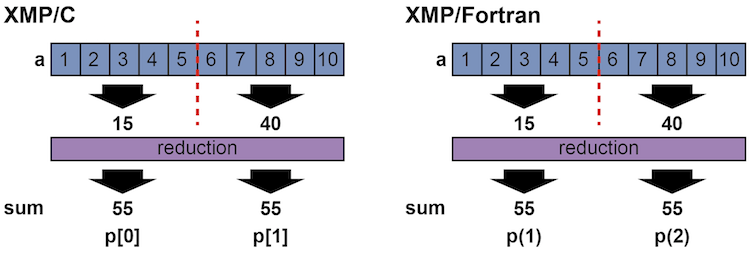
\includegraphics[width=\textwidth]{figs/reduction2.png}
  \caption{Example of reduction computation (2).}
\end{figure}

Operations that can be specified as an operator in a \|reduction| clause
are limited to the following associative ones.

\begin{Cexample}
+
*
-
&
|
^
&&
||
max
min
firstmax
firstmin
lastmax
lastmin
\end{Cexample}

\begin{Fexample}
+
*
-
.and.
.or.
.eqv.
.neqv.
max
min
iand
ior
ieor
firstmax
firstmin
lastmax
lastmin
\end{Fexample}

\begin{mynote}
  The total result is calculated by combining the partial results on all
  {\nodes}. The ordering of the combination is unspecified.
%
  Hence, if the target variable is a type of floating
  point (e.g. \|float| in XMP/C or \|real| in XMP/Fortran), the
  difference of the order can make a little bit
  difference in the result value from that in the original serial
  execution.
\end{mynote}


\subsubsection{Parallelizing Nested Loop}

Parallelization of nested loops can be specified similarly to a single
one, as follows.

\begin{XCexample}
#pragma xmp nodes p[2][2]
#pragma xmp template t[10][10]
#pragma xmp distribute t[block][block] onto p

int main(){
  int a[10][10];
#pragma xmp align a[i][j] with t[i][j]

#pragma xmp loop on t[i][j]
  for(int i=0;i<10;i++)
    for(int j=0;j<10;j++)
      a[i][j] = i*10+j;

  return 0;
}
\end{XCexample}

\begin{XFexample}
program main
!$xmp nodes p(2,2)
!$xmp template t(10,10)
!$xmp distribute t(block,block) onto p
  integer :: a(10,10)
!$xmp align a(j,i) with t(j,i)

!$xmp loop on t(j,i)
  do i=1, 10
    do j=1, 10
      a(j,i) = i*10+j
    enddo
  enddo

end program main
\end{XFexample}


\subsection{{\tt array} Construct}

The \|array| construct is for work mapping of array assignment statements.

\begin{XCexample}
#pragma xmp align a[i] with t[i]
  :
#pragma xmp array on t[0:N]
a[0:N] = 1.0;
\end{XCexample}

\begin{XFexample}
!$xmp align a(i) with t(i)
  :
!$xmp array on t(1:N)
a(1:N) = 1.0
\end{XFexample}

The above is equivalent to the below.

\begin{XCexample}
#pragma xmp align a[i] with t[i]
  :
#pragma xmp loop on t[i]
for(int i=0;i<N;i++)
  a[i] = 1.0;
\end{XCexample}

\begin{XFexample}
!$xmp align a(i) with t(i)
  :
!$xmp loop on t(i)
do i=1, N
  a(i) = 1.0
enddo
\end{XFexample}

This construct can also be applied to multi-dimensional arrays.
% The
% triplet notation enables specifying operations for all elements of the
% array.

\begin{XCexample}
#pragma xmp align a[i][j] with t[i][j]
  :
#pragma xmp array on t[:][:]
a[:][:] = 1.0;
\end{XCexample}

\begin{XFexample}
!$xmp align a(j,i) with t(j,i)
  :
!$xmp array on t(:,:)
a(:,:) = 1.0
\end{XFexample}

\begin{mynote}
  The {\template} appearing in the \|on| clause must have the same shape as
  the arrays in the following statement. The right-hand side value in
  this construct must be identical among all {\nodes} because the \|array|
  construct is a {\bf global} (i.e. collective) operation.
\end{mynote}

\section{Data Communication}

\subsection{{\bf shadow} Directive and {\bf reflect} Construct}

Stencil computation frequently appears in scientific computations,
where array elements \|a[i-1]| and \|a[i+1]| are referenced to update
\|a[i]|. If \|a[i]| is on the boundary region of a block-distributed
array on a node, \|a[i+1]| may reside on another (neighboring) node.

Since it involves large overhead to copy \|a[i+1]| from the neighboring node to
update each \|a[i]|, a technique of copying collectively elements on the
neighboring node to the area added to the distributed array on each node
is usually adopted. In XMP, such additional area is called ``shadow.''

\subsubsection{Declaring Shadow}

%\paragraph{Widths of lower/upper bounds are the same}

Shadow areas can be declared with the \|shadow| directive. In the example
below, an array \|a| has shadow areas of width one on both the lower and
upper bounds.

\begin{XCexample}
#pragma xmp nodes p[4]
#pragma xmp template t[16]
#pragma xmp distribute t[block] onto p
double a[16];
#pragma xmp align a[i] with t[i]
#pragma xmp shadow a[1]
\end{XCexample}

\begin{XFexample}
!$xmp nodes p(4)
!$xmp template t(16)
!$xmp distribute t(block) onto p
real :: a(16)
!$xmp align a(i) with t(i)
!$xmp shadow a(1)
\end{XFexample}

\begin{figure}
  \centering
  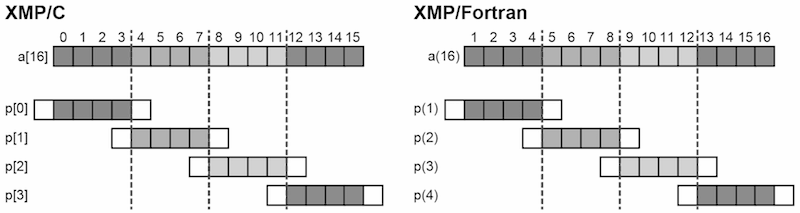
\includegraphics[width=\textwidth]{figs/shadow.png}
\end{figure}

In the figure above, colored elements are those that each node owns and
white ones are shadow.

\begin{mynote}
  Arrays distributed in a cyclic manner cannot have shadow.  
\end{mynote}

%\paragraph{Widths of lower/upper bounds are different}

In some programs, it is natural that the widths of the shadow area on
the lower and upper bounds are different. There is also a case where the
shadow area exists only on either of the bounds. In the example below,
it is declared that a distributed array \|a| has a shadow area of width
one only on the upper bound.

\begin{XCexample}
#pragma xmp nodes p[4]
#pragma xmp template t[16]
#pragma xmp distribute t(block) onto p
double a[16];
#pragma xmp align a[i] with t[i]
#pragma xmp shadow a[0:1]
\end{XCexample}

\begin{XFexample}
!$xmp nodes p(4)
!$xmp template t(16)
!$xmp distribute t(block) onto p
real :: a(16)
!$xmp align a(i) with t(i)
!$xmp shadow a(0:1)
\end{XFexample}

\begin{figure}
  \centering
  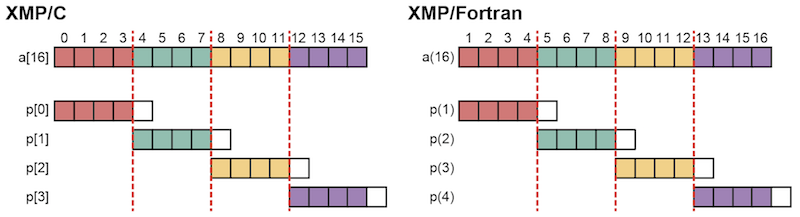
\includegraphics[width=\textwidth]{figs/shadow_uneven.png}
\end{figure}

The values on the left- and right-hand sides of a colon designate the
widths on the lower and upper bounds, respectively.

\subsubsection{Updating Shadow}

%\paragraph{General}

To copy data to shadow areas from neighboring nodes, use the \|reflect|
construct. In the example below, the shadow areas of an array \|a| that
are of width one on both the upper and lower bounds are updated.

\begin{XCexample}
#pragma xmp reflect (a)

#pragma xmp loop on t[i]
for(int i=1;i<15;i++)
  a[i] = (a[i-1] + a[i] + a[i+1])/3;
\end{XCexample}

\begin{XFexample}
!$xmp reflect (a)

!xmp loop on t(i)
do i=2, 15
  a(i) = (a(i-1) + a(i) + a(i+1))/3
enddo
\end{XFexample}

\begin{figure}
  \centering
  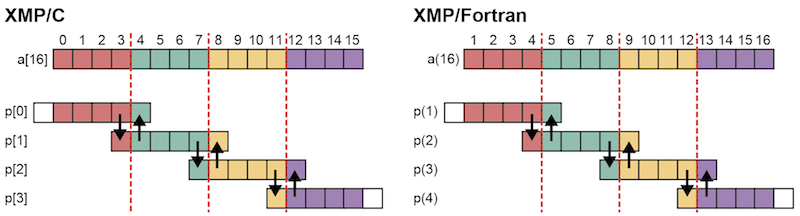
\includegraphics[width=\textwidth]{figs/reflect.png}
\end{figure}

With this reflect directive, in XMP/C, node \|p[1]| sends an element
\|a[4]| to the shadow area on the upper bound on node \|p[0]| and
\|a[7]| to the shadow area on the lower bound on \|p[2]|; \|p[0]| sends
an element \|a[3]| to the shadow area on the lower bound on \|p[1]|, and
\|p[2]| sends \|a[8]| to the shadow area on the upper bound on \|p[1]|.

Similarly, in XMP/Fortran, node \|p(2)| sends an element \|a(5)| to the
shadow area on the upper bound on node \|p(1)| and \|a(8)| to the shadow
area on the lower bound on \|p(3)|; \|p(1)| sends an element \|a(4)| to
the shadow area on the lower bound on \|p(2)|, and \|p(3)| sends \|a(9)|
to the shadow area on the upper bound on \|p(2)|.

%\paragraph{Specify Width}

The default behavior of a reflect directive is to update the whole of
the shadow area declared by the \|shadow| directive. However, there are
some cases where a specific part of the shadow area is to be updated to
reduce the communication size at a point of the code.

To update only a specific part of the shadow area, add the \|width|
clause to the \|reflect| directive.

The values on the left- and right-hand sides of a colon in the \|width|
clause designate the widths on the lower and upper bounds to be updated,
respectively. In the example below, only the shadow area on the upper
bound is updated.

\begin{XCexample}
#pragma xmp reflect (a) width(0:1)
\end{XCexample}

\begin{XFexample}
!$xmp reflect (a) width(0:1)
\end{XFexample}

\begin{figure}
  \centering
  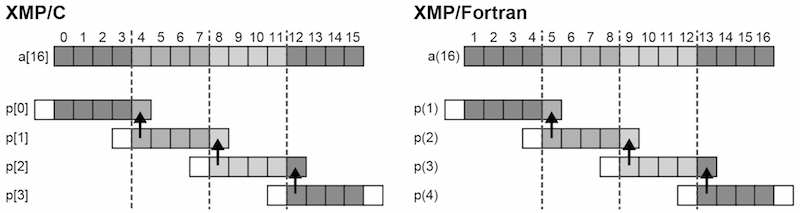
\includegraphics[width=\textwidth]{figs/reflect_width.png}
\end{figure}

\begin{mynote}
  If the widths of the shadow areas to be updated on the upper and lower 
  bounds are equal, that is, for example, \|width(1:1)|, you can
  abbreviate it as \|width(1)|.
\end{mynote}

\begin{mynote}
  It is not possible to update the shadow area on a particular node
  because \|reflect| is a collective operation.
\end{mynote}

% If no shadow area is specified on the lower bound, the reflect directive
% does not update it with or without a width clause. The below figure
% illustrates the behavior of a reflect directive for a distributed array
% a having a shadow area of width one only on the upper bound.

% \begin{figure}
%   \centering
%   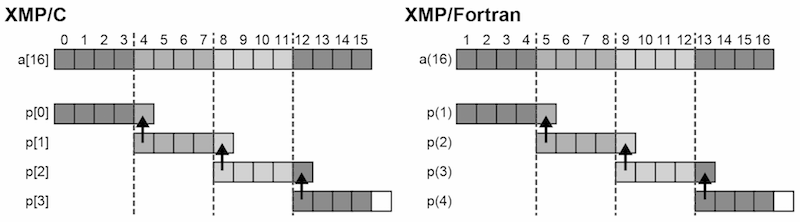
\includegraphics{figs/reflect_uneven.png}
% \end{figure}

%\paragraph{Update periodic shadow}

The \|reflect| directive does not update either the shadow area on the
lower bound on the leading node or that on the upper bound on the last
node. However, the values in such areas are needed for stencil
computation if the computation needs a periodic boundary condition.

To update such areas, add a \|periodic| qualifier into a width
clause. Let’s look at the following example where an array \|a| having
shadow areas of width one on both the lower and upper bounds appears.

\begin{XCexample}
#pragma xmp reflect (a) width(/periodic/1:1)
\end{XCexample}

\begin{XFexample}
!$xmp reflect (a) width(/periodic/1:1)
\end{XFexample}

\begin{figure}
  \centering
  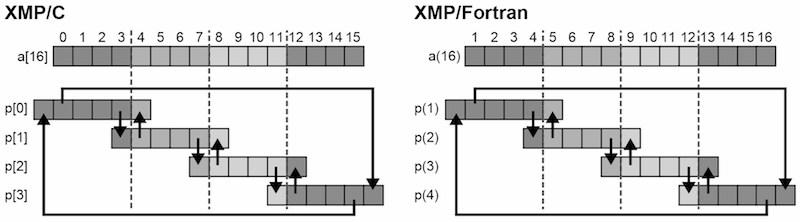
\includegraphics[width=\textwidth]{figs/reflect_periodic.png}
\end{figure}

The \|periodic| qualifier has the following effects, in addition to that of
a normal \|reflect| directive: in XMP/C, node \|p[0]| sends an element
\|a[0]| to the shadow area on the upper bound on node \|p[3]|, and
\|p[3]| sends \|a[15]| to the shadow area on the lower bound on \|p[0]|;
in XMP/Fortran, node \|p(1)| sends an element \|a(1)| to the shadow area
on the upper bound on node \|p(4)|, and \|p(4)| sends \|a(16)| to the
shadow area on the lower bound on \|p(1)|.

% \begin{mynote}
%   If the widths of the shadow areas to be updated on
% the upper and lower 
% bounds are equal, as shown by width(/periodic/1:1) in the above example,
% you can abbreviate it as width(/periodic/1).
% \end{mynote}

%\subsubsection{Multi-dimensional Shadow}

The \|shadow| directive and \|reflect| construct can be applied to
array distributed in multiple dimensions. The following programs are the
examples for two-dimensional distribution.

\begin{XCexample}
#pragma xmp nodes p[3][3]
#pragma xmp template t[9][9]
#pragma xmp distribute t[block][block] onto p
double a[9][9];
#pragma xmp align a[i][j] with t[i][j]
#pragma xmp shadow a[1][1]
   :
#pragma xmp reflect (a)
\end{XCexample}

\begin{XFexample}
!$xmp nodes p(3,3)
!$xmp template t(9,9)
!$xmp distribute t(block,block) onto p
real :: a(9,9)
!$xmp align a(j,i) with t(j,i)
!$xmp shadow a(1,1)
   :
!$xmp reflect (a)
\end{XFexample}

\begin{figure}
  \centering
  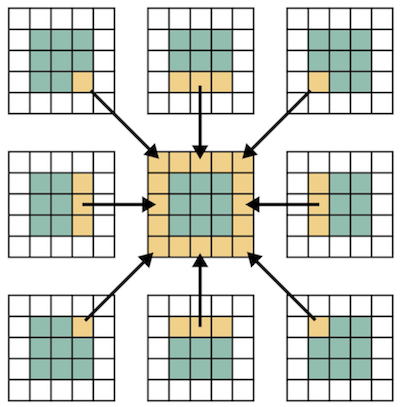
\includegraphics{figs/multi1.png}
\end{figure}

The central node receives data from the surrounding eight
nodes to update its shadow areas. The shadow areas of the other nodes
are also updated, which is omitted in the figure.

For some applications, data from ordinal directions are not
necessary. In such a case, the data communication from/to the ordinal
directions can be avoided by adding an \|orthogonal| clause to a
\|reflect| construct.

\begin{XCexample}
#pragma xmp reflect (a) orthogonal
\end{XCexample}

\begin{XFexample}
!$xmp reflect (a) orthogonal
\end{XFexample}

\begin{figure}
  \centering
  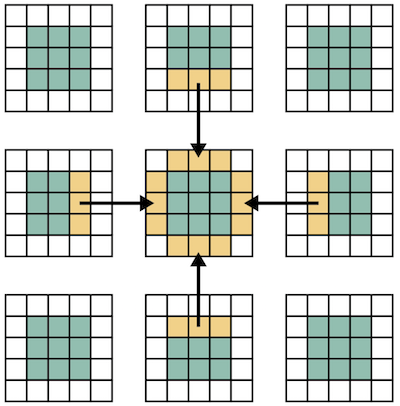
\includegraphics{figs/multi_orthogonal.png}
\end{figure}

\begin{mynote}
The orthogonal clause is effective only for arrays
more than one 
dimension of which is distributed.
\end{mynote}

Besides, you can also add shadow areas to only specified dimension.

\begin{XCexample}
#pragma xmp nodes p[3]
#pragma xmp template t[9]
#pragma xmp distribute t[block] onto p
double a[9][9];
#pragma xmp align a[i][*] with t[i]
#pragma xmp shadow a[1][0]
  :
#pragma xmp reflect (a)
\end{XCexample}

\begin{XFexample}
!$xmp nodes p[3]
!$xmp template t[9]
!$xmp distribute t[block] onto p
real :: a(9,9)
!$xmp align a(*,i) with t(i)
!$xmp shadow a(0,1)
  :
!$xmp reflect (a)
\end{XFexample}

\begin{figure}
  \centering
  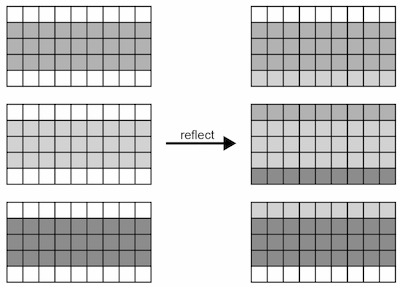
\includegraphics{figs/1of2.png}
\end{figure}

For the array \|a|, 0 is specified as the shadow width in the dimensions
which are not distributed.


\subsection{{\tt gmove} Construct}

You can specify a communication for distributed arrays in the form of
assignment statements by using the \|gmove| construct.

There are three modes of \|gmove|; ``collective mode,'' ``in mode,'' and
``out mode.''
% While collective mode executes two-sided communication among the
% executing nodes, in/out modes execute one-sided communication among
% tasks with a task directive. While in mode uses get communication, out
% mode uses put communication.

\subsubsection{Collective Mode}

%\paragraph{Distributed array}

% Copying a part of array a to array b. Array assignment statements in a
% gmove construct uses triplet.

The copy operation involved by a {\it collective} \|gmove| is performed
collectively, and results in implicit synchronization among the 
executing nodes.

\begin{XCexample}
#pragma xmp nodes p[4]
#pragma xmp template t[16]
#pragma xmp distribute t[block] onto p
int a[16], b[16];
#pragma xmp align a[i] with t[i]
#pragma xmp align b[i] with t[i]
     :
#pragma xmp gmove
  a[9:5] = b[0:5];
\end{XCexample}

\begin{XFexample}
!$xmp nodes p(4)
!$xmp template t(16)
!$xmp distribute t(block) onto p
integer :: a(16), b(16)
!$xmp align a(i) with t(i)
!$xmp align b(i) with t(i)
     :
!$xmp gmove
  a(10:14) = b(1:5)
\end{XFexample}

\begin{figure}
  \centering
  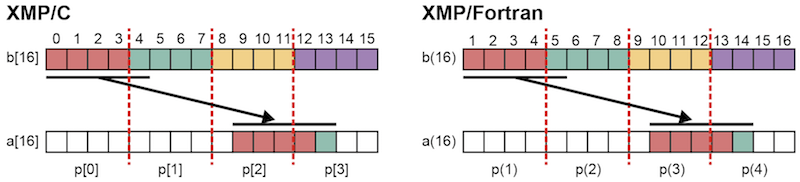
\includegraphics[width=\textwidth]{figs/gmove.png}
\end{figure}

In XMP/C, \|p[0]| sends \|b[0]|-\|b[3]| to \|p[2]|-\|p[3]|, and \|p[1]|
sends \|b[4]| to \|p[3]|. Similarly, in XMP/Fortran, \|p(1)| sends
\|b(1)|-\|b(4)| to \|p(3)|-\|p(4)|, and \|p(2)| sends \|b(5)| to \|p(4)|.

\begin{XCexample}
#pragma xmp nodes p[4]
#pragma xmp template t1[16]
#pragma xmp template t2[16]
#pragma xmp distribute t1[cyclic] onto p
#pragma xmp distribute t2[block] onto p
int a[16], b[16];
#pragma xmp align a[i] with t1[i]
#pragma xmp align b[i] with t2[i]
     :
#pragma xmp gmove
  a[9:5] = b[0:5];
\end{XCexample}

\begin{XFexample}
!$xmp nodes p(4)
!$xmp template t1(16)
!$xmp template t2(16)
!$xmp distribute t1(cyclic) onto p
!$xmp distribute t2(block) onto p
integer :: a(16), b(16)
!$xmp align a(i) with t1(i)
!$xmp align b(i) with t2(i)
     :
!$xmp gmove
  a(10:14) = b(1:5)
\end{XFexample}

\begin{figure}
  \centering
  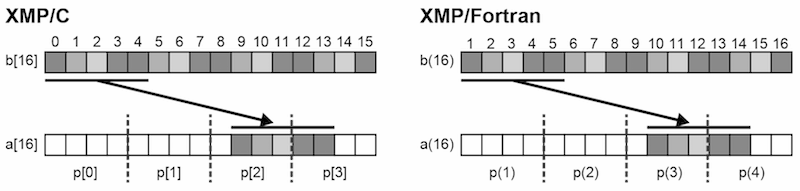
\includegraphics[width=\textwidth]{figs/gmove_cyclic.png}
\end{figure}

While array \|a| is distributed in a cyclic manner, array \|b| is
distributed in a block manner.

In XMP/C, \|p[0]| sends \|b[0]| and \|b[4]| to \|p[2]| and
\|p[3]|. \|p[1]| sends \|b[1]| to \|p[2]|. Each element of \|p[2]| and
\|p[3]| will be copied locally. Similarly, in XMP/Fortran, \|p(1)| sends
\|b(1)| and \|b(5)| to \|p(3)| and \|p(4)|. \|p(2)| sends \|b(2)| to
\|p(3)|. Each element of \|p(3)| and \|p(4)| will be copied locally.

% \begin{mynote}
%   If the number of elements specified on the
% right-hand side is other than one, it will not work properly if the
%   number of elements differs between the right-hand side and the
%   left-hand side.
% \end{mynote}

By using this method, the shape of a distributed array can be ``changed''
during computation.

\begin{XCexample}
#pragma xmp nodes p[4]
#pragma xmp template t1[16]
#pragma xmp template t2[16]
int W[4] = {2,4,8,2};
#pragma xmp distribute t1[gblock(W)] onto p
#pragma xmp distribute t2[block] onto p
int a[16], b[16];
#pragma xmp align a[i] with t1[i]
#pragma xmp align b[i] with t2[i]
     :
#pragma xmp gmove
  a[:] = b[:];
\end{XCexample}

\begin{XFexample}
!$xmp nodes p(4)
!$xmp template t1(16)
!$xmp template t2(16)
integer :: W(4) = (/2,4,7,3/)
!$xmp distribute t1(gblock(W)) onto p
!$xmp distribute t2(block) onto p
integer :: a(16), b(16)
!$xmp align a(i) with t1(i)
!$xmp align b(i) with t2(i)
     :
!$xmp gmove
  a(:) = b(:)
\end{XFexample}

\begin{figure}
  \centering
  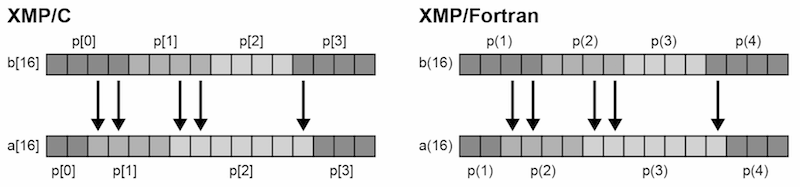
\includegraphics[width=\textwidth]{figs/gmove_change.png}
\end{figure}

In this example, copying all elements of array \|b| that is distributed in
a block manner to array \|a| that is distributed in a generalized-block
manner.
%
For arrays \|a| and \|b|, communication occurs if corresponding elements
reside in different nodes (arrows illustrate communication between nodes in
the figures).

%\paragraph{Scalar}

In an assignment statement, if a scalar (i.e. one element of an array or
a variable) is specified on the right-hand side and an array section are
specified on the left-hand side, the operation will be broadcast
communication.

\begin{XCexample}
#pragma xmp nodes p[4]
#pragma xmp template t[16]
#pragma xmp distribute t[block] onto p
int a[16], b[16];
#pragma xmp align a[i] with t[i]
#pragma xmp align b[i] with t[i]
     :
#pragma xmp gmove
  a[9:5] = b[0];
\end{XCexample}

\begin{XFexample}
!$xmp nodes p(4)
!$xmp template t(16)
!$xmp distribute t(block) onto p
integer :: a(16), b(16)
!$xmp align a(i) with t(i)
!$xmp align b(i) with t(i)
     :
!$xmp gmove
  a(10:14) = b(1)
\end{XFexample}

\begin{figure}
  \centering
  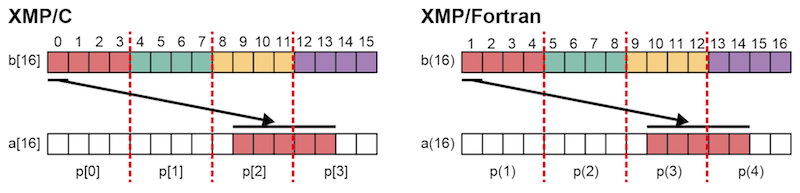
\includegraphics[width=\textwidth]{figs/gmove_one_element.png}
\end{figure}

In this example, in XMP/C, an array element \|b[0]| of node \|p[0]| will be
broadcasted to the specified array section on node \|p[2]| and
\|p[3]|. Similarly, in XMP/Fortran, an array element \|b(1)| of node
\|p(1)| will be broadcasted to the specified array section on node \|p(3)| and \|p(4)|.

%\paragraph{Duplicated array and scalar}

Not only distributed arrays but also replicated arrays can be specified
on the right-hand side.

\begin{XCexample}
 #pragma xmp nodes p[4]
 #pragma xmp template t[16]
 #pragma xmp distribute t[block] onto p
 int a[16], b[16], c;
 #pragma xmp align a[i] with t[i]
      :
#pragma xmp gmove
   a[9:5] = b[0:5];
\end{XCexample}

\begin{XFexample}
 !$xmp nodes p(4)
 !$xmp template t(16)
 !$xmp distribute t(block) onto p
 integer :: a(16), b(16), c
 !$xmp align a(i) with t(i)
      :
!$xmp gmove
   a(10:14) = b(1:5)
\end{XFexample}

In this example, a replicated array \|b| is locally copied to
distributed array \|a| without communication.

%\paragraph{Distributed array with different dimension}

\begin{XCexample}
#pragma xmp nodes p[4]
#pragma xmp template t1[8]
#pragma xmp template t2[16]
#pragma xmp distribute t1[block] onto p
#pragma xmp distribute t2[block] onto p
int a[8][16], b[8][16];
#pragma xmp align a[i][*] with t1[i]
#pragma xmp align b[*][i] with t2[i]
     :
#pragma xmp gmove
  a[0][:] = b[0][:];
\end{XCexample}

\begin{XFexample}
!$xmp nodes p(4)
!$xmp template t1(8)
!$xmp template t2(16)
!$xmp distribute t1(block) onto p
!$xmp distribute t2(block) onto p
integer :: a(16,8), b(8,16)
!$xmp align a(*,i) with t1(i)
!$xmp align b(i,*) with t2(i)
     :
#pragma xmp gmove
  a(:,1) = b(:,1)
\end{XFexample}

\begin{figure}
  \centering
  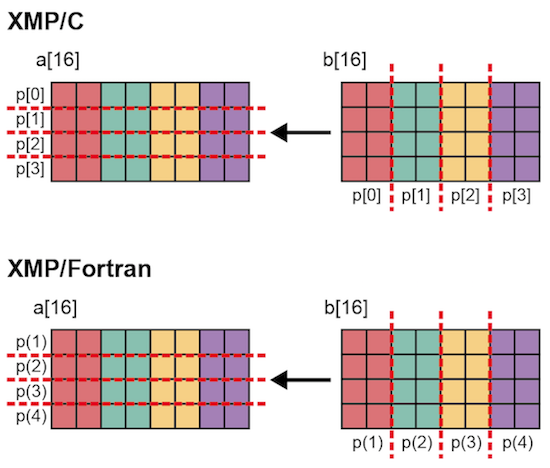
\includegraphics{figs/gmove_different.png}
\end{figure}

In this example, in XMP/C, \|b[0][0:2]| on \|p[0]|, \|b[0][2:2]| of
\|p[1]|, \|b[0][4:2]| on \|p[2]| and \|b[0][6:2]| on \|p[3]| are copied
to \|a[0][:]| on \|p[0]|. Similarly, in XMP/Fortran, \|b(1:2,1)| on
\|p(1)|, \|b(3:4,1)| of \|p(2)|, \|b(5:6,1)| on \|p(3)| and \|b(7:8,1)|
on \|p(4)| are copied to \|a(:,1)| on \|p(1)|.


\subsubsection{In Mode}

%It operates as in mode by setting in clause to gmove directive.

The right-hand side data of the assignment, all or part of which may
reside outside the executing node set, can be transferred from its owner
nodes to the executing nodes by an {\it in} \|gmove|.

\begin{XCexample}
#pragma xmp nodes p[4]
#pragma xmp template t[4]
#pragma xmp distribute t[block] onto p
double a[4], b[4];
#pragma xmp align a[i] with t[i]
#pragma xmp align b[i] with t[i]
   :
#pragma xmp task on p[0:2]
#pragma xmp gmove in
  a[0:2] = b[2:2]
#pragma xmp end task
\end{XCexample}

\begin{XFexample}
!$xmp nodes p(4)
!$xmp template t(4)
!$xmp distribute t(block) onto p
real :: a(4), b(4)
!$xmp align a(i) with t(i)
!$xmp align b(i) with t(i)
   :
!$xmp task on p(1:2)
!$xmp gmove in
  a(1:2) = b(3:4)
!$xmp end task
\end{XFexample}

In this example, the \|task| directive divides four nodes into
two sets, the first-half and the second-half. A \|gmove| construct that
is in an {\it in} mode copies data using a {\it get} operation from
the second-half node to the first-half node.

\begin{figure}
  \centering
  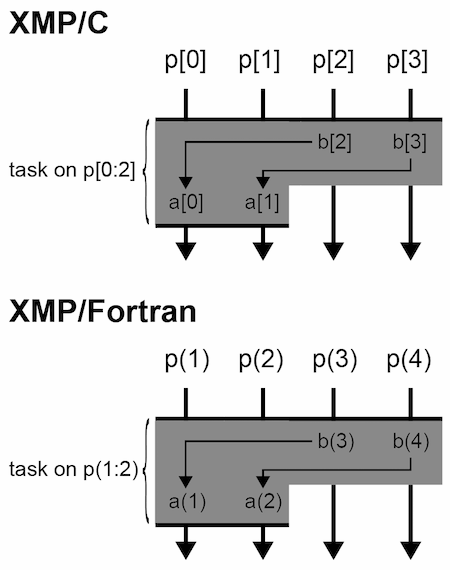
\includegraphics{figs/gmove_in.png}
\end{figure}


\subsubsection{Out Mode}

The left-hand side data of the assignment, all or part of which may
reside outside the executing node set, can be transferred from the
executing nodes to its owner nodes by an {\it out} \|gmove| construct.

\begin{XCexample}
#pragma xmp nodes p[4]
#pragma xmp template t[4]
#pragma xmp distribute t[block] onto p
double a[4], b[4];
#pragma xmp align a[i] with t[i]
#pragma xmp align b[i] with t[i]
   :
#pragma xmp task on p[0:2]
#pragma xmp gmove out
  b[2:2] = a[0:2]
#pragma xmp end task
\end{XCexample}

\begin{XFexample}
!$xmp nodes p(4)
!$xmp template t(4)
!$xmp distribute t(block) onto p
real :: a(4), b(4)
!$xmp align a(i) with t(i)
!$xmp align b(i) with t(i)
   :
!$xmp task on p(1:2)
!$xmp gmove out
  b(3:4) = a(1:2)
!$xmp end task
\end{XFexample}

A \|gmove| construct that is in {\it out} mode copies data using a {\it put}
communication from the first-half nodes to the second-half nodes.

\begin{figure}
  \centering
  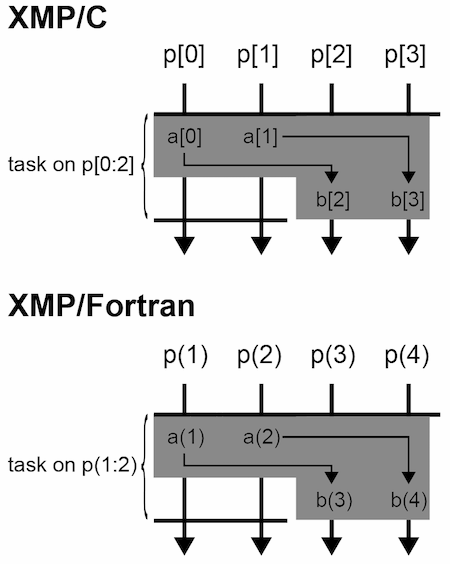
\includegraphics{figs/gmove_out.png}
\end{figure}


\subsection{{\bf barrier} Construct}

The \|barrier| construct executes a barrier synchronization.

\begin{XCexample}
#pragma xmp barrier
\end{XCexample}

\begin{XFexample}
!$xmp barrier
\end{XFexample}

You can specify a node set on which the barrier synchroniation is to be
performed by using the \|on| clause. In the below example, a barrier
synchronization is performed among the first two nodes of \|p|.

\begin{XCexample}
#pragma xmp barrier on p[0:2]
\end{XCexample}

\begin{XFexample}
!$xmp barrier on p(1:2)
\end{XFexample}


\subsection{{\bf reduction} Construct}

This construct performs a {\it reduction} operation. It has the same
meaning as the \|reduction| clause of the \|loop| construct, but this
construct can be specified anywhere as an {\it executable} construct.

\begin{XCexample}
#pragma xmp nodes p[4]
  :
sum = xmpc_node_num() + 1;
#pragma xmp reduction (+:sum)
\end{XCexample}

\begin{XFexample}
!$xmp nodes p(4)
  :
sum = xmp_node_num()
!$xmp reduction (+:sum)
\end{XFexample}

\begin{figure}
  \centering
  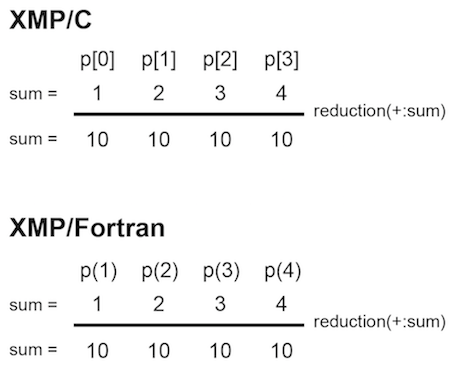
\includegraphics{figs/reduction.png}
\end{figure}

You can specify the executing node set by using the \|on| clause. In the
below example, only the values on the last two of the four nodes are
targeted by the \|reduction| construct.

\begin{XCexample}
#pragma xmp nodes p[4]
  :
sum = xmpc_node_num() + 1;
#pragma xmp reduction (+:sum) on p[2:2]
\end{XCexample}

\begin{XFexample}
!$xmp nodes p(4)
  :
 sum = xmp_node_num()
 !$xmp reduction (+:sum) on p(3:4)
\end{XFexample}

\begin{figure}
  \centering
  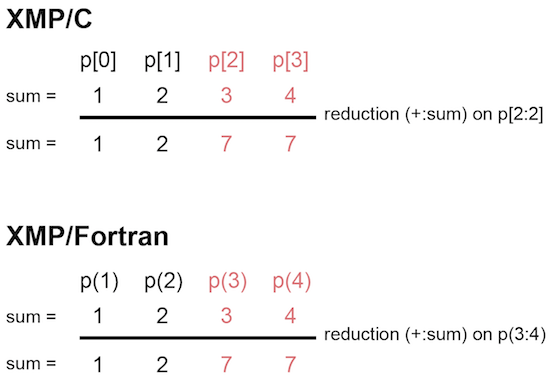
\includegraphics{figs/reduction_on.png}
\end{figure}

The operators you can use in the \|reduction| construct are as follows:

\begin{XCexample}
+
*
-
&
|
^
&&
||
max
min
\end{XCexample}

\begin{XFexample}
+
*
-
.and.
.or.
.eqv.
.neqv.
max
min
iand
ior
ieor
\end{XFexample}

\begin{mynote}
% Since the \|reduction| clause needs a loop statement,
% operators of
% firstmax, firstmin, lastmax, and lastmin are required. But, since the
% reduction directive does not need a loop statement, there are no such
% operators.
  In contrast to the \|reduction| clause of the \|loop| construct, which
  precedes loops, the \|reduction| construct does not accept operators of
  \|firstmax|, \|firstmin|, \|lastmax|, and \|lastmin|.
\end{mynote}

\begin{mynote}
  Similar to the \|reduction| clause, the \|reduction| construct may
  generate slightly different results in a parallel execution from in a
  sequential execution, because the results depends on the order of
  associating the value.
\end{mynote}


\subsection{{\bf bcast} Construct}

The \|bcast| construct broadcasts the values of the variables on the
node specified by the \|from| clause, that is, the {\it root node}, to
the node set specified by the \|on| clause.
%
If there is no \|from| clause, the first node of the executing node
set is selected as the root node.
%
If there is no \|on| clause, the current executing node set of the
construct is selected as the executing node set.

In the below example, the first node of the node set \|p| is the root
node.

\begin{XCexample}
#pragma xmp nodes p[4]
  :
num = xmpc_node_num() + 1;
#pragma xmp bcast (num)
\end{XCexample}

\begin{XFexample}
!$xmp nodes p(4)
  :
num = xmp_node_num()
!$xmp bcast (num)
\end{XFexample}

\begin{figure}
  \centering
  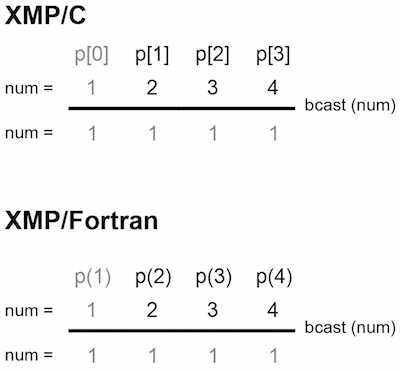
\includegraphics{figs/bcast.png}
\end{figure}

In the below example, the last node is the \|from| clause.

\begin{XCexample}
#pragma xmp nodes p[4]
  :
num = xmpc_node_num() + 1;
#pragma xmp bcast (num) from p[3]
\end{XCexample}

\begin{XFexample}
!$xmp nodes p(4)
  :
num = xmp_node_num()
!$xmp bcast (num) from p(4)
\end{XFexample}

\begin{figure}
  \centering
  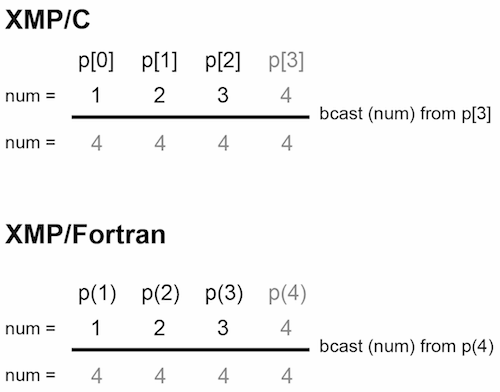
\includegraphics{figs/bcast_from.png}
\end{figure}

In the below example, only the last three of four nodes
are the executing node set of the \|bcast| construct.

\begin{XCexample}
#pragma xmp nodes p[4]
  :
sum = xmpc_node_num() + 1;
#pragma xmp bcast (num) from p[3] on p[1:3]
\end{XCexample}

\begin{XFexample}
!$xmp nodes p(4)
  :
 sum = xmp_node_num()
 !$xmp bcast (num) from p(4) on p(2:4)
\end{XFexample}

\begin{figure}
  \centering
  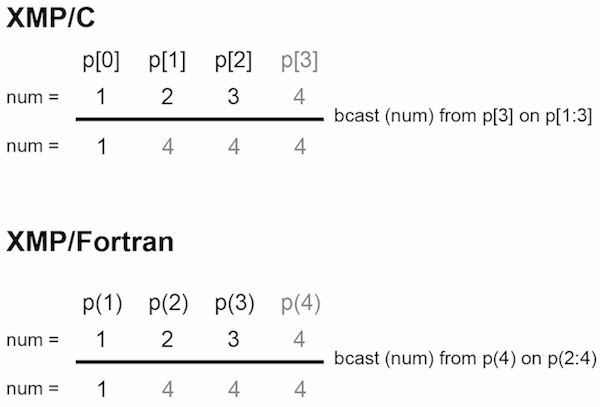
\includegraphics{figs/bcast_from_on.png}
\end{figure}


\subsection{{\bf wait\_async} Construct}

Communication directives (i.e. \|reflect|, \|gmove|, \|reduction|,
\|bcast|, \|reduce_shadow|) can perform asynchronous communication if
the \|async| clause is added. The \|wait_async| construct is used to
guarantee the completion of asynchronous communication.

\begin{XCexample}
#pragma xmp bcast (num) async(1)
    :
#pragma xmp wait_async (1)
\end{XCexample}

\begin{XFexample}
!$xmp bcast (num) async(1)
        :
!$xmp wait_async (1)
\end{XFexample}

Since the \|bcast| directive has an \|async| clause, communication may
not be completed immediately after the \|bcast| directive. The
completion of that communication is guaranteed with the \|wait_async|
construct having the same value as that of the \|async| clause.
%
Therefore, between the \|bcast| construct and the \|wait_async|
constructs, you may not reference the target variable of the \|bcast|
directive.

\begin{myhint}
By performing computation without a dependency
relationship with the variable specified by the bcast directive after
the bcast directive, overlap of communication and computation can be
performed, so the total computation time may be small.
\end{myhint}

\begin{mynote}
Expressions that can be specified in the \|async| clause are
of type int, in XMP/C, or integer, in XMP/Fortran.
\end{mynote}


\subsection{{\bf reduce\_shadow} Construct}

The \|reduce_shadow| directive adds the value of a shadow object to the
corresponding data object of the array.

\begin{XCexample}
#pragma xmp nodes p[2]
#pragma xmp template t[8]
#pragma xmp distribute t[block] onto p
int a[8];
#pragma xmp align a[i] with t[i]
#pragma xmp shadow a[1]
 :
#pragma xmp loop on t[i]
  for(int i=0;i<8;i++)
    a[i] = i+1;

#pragma xmp reflect (a)
#pragma xmp reduce_shadow (a)
\end{XCexample}

\begin{XFexample}
!$xmp nodes p(2)
!$xmp template t(8)
!$xmp distribute t(block) onto p
  integer a(8)
!$xmp align a(i) with t(i)
!$xmp shadow a(1)

!$xmp loop on t(i)
  do i=1, 8
    a(i) = i
  enddo

!$xmp reflect (a)
!$xmp reduce_shadow (a)
\end{XFexample}

% The \|shadow| directive adds a shadow are of width one to the
% distributed array \|a| of each node. Next, the \|reflect| construct
% updates the shadow area. Finally, the \|reduce_shadow| construct adds
% the value of the shadow to the value of the source element.

For the above example, in XMP/C, \|a[3]| on \|p[0]| has a value of eight,
and \|a[4]| on \|p[1]| has a value of ten. Similarly, in XMP/Fortran,
\|a(4)| of \|p(1)| has a value of eight, and \|a(5)| on \|p(2)| has a
value of ten.

\begin{figure}
  \centering
  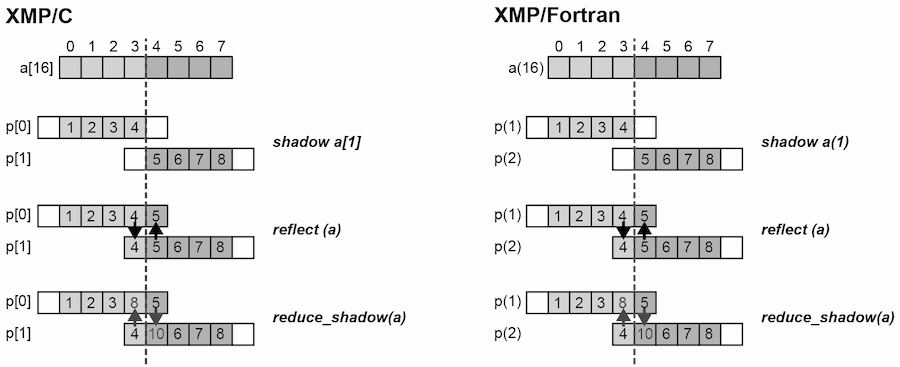
\includegraphics[width=\textwidth]{figs/reduce_shadow.png}
\end{figure}

You can add the \|periodic| modifier to the \|width| clause to update
the shadow area periodically.

\begin{XCexample}
#pragma xmp reflect (a) width(/periodic/1)
#pragma xmp reduce_shadow (a) width(/periodic/1)
\end{XCexample}

\begin{XFexample}
!$xmp reflect (a) width(/periodic/1)
!$xmp reduce_shadow (a) width(/periodic/1)
\end{XFexample}

\begin{figure}
  \centering
  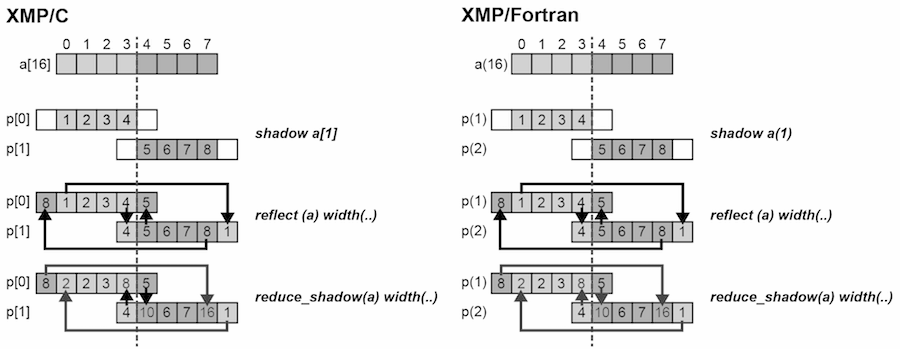
\includegraphics[width=\textwidth]{figs/reduce_shadow_periodic.png}
\end{figure}

In addition to the first example, in XMP/C, \|a[0]| on \|p[0]| has a
value of two, and \|a[7]| on \|p[1]| has a value of 16. Similarly, in
XMP/Fortran, \|a(1)| in \|p(1)| has a value of two, and \|a(8)| in
\|p(2)| has a value of 16.
\section{Local-view Programming}

\subsection{Introduction}

The programmer can use {\coarrays} to specify one-sided communication in
the local-view model.
% In XMP, put/get communication and some
% synchronization functions are supported.

Depending on the environment, such one-sided communication might achieve
better performance than global communication in the global-view model.
%
However, it is more difficult and complicated to
write parallel programs in the local-view model because the programmer
must specify every detail of
parallelization, such as data mapping, work mapping, and communication.

% XMP/Fortran supports coarray as its base language Fortran 2008. Coarray
% in XMP/C has its own original syntax since the C language does not support
% Coarray.

The {\coarray} feature in XMP/Fortran is upward-compatibile with that in
Fortran 2008; that in XMP/C is defined as an extension to the base
language.

An execution entity in local-view XMP programs is referred to as an 
``image'' while a {\node} in global-view ones.
%
These two words have almost the same meaning in XMP.

\subsection{Coarray Declaration}

\begin{XCexample}
int a[10]:[*];
\end{XCexample}

\begin{XFexample}
integer a(10)[*]
\end{XFexample}

In XMP/C, the programmer declares a {\coarray} by adding ``\|:[*]|''
after the array declaration. In XMP/Fortran, the programmer declares a
{\coarray} by adding ``\|[*]|'' after the array declaration.
%The asterisk symbol is used in both languages.

\begin{mynote}
  Based on Fortran 2008, {\coarrays} should have the same size among all
  images.
\end{mynote}

{\bf Coarrays} can be accessed in expressions by remote images as well the
local image.


\subsection{Put Communication}

When a {\coarray} appears in the left-hand side of an
assignment statement, it involves {\it put} communication.

\begin{XCexample}
int a[10]:[*], b[10];

if (xmpc_this_image() == 0)
  a[0:3]:[1] = b[3:3];
\end{XCexample}

\begin{XFexample}
integer a(10)[*]
integer b(10)

if (this_image() == 1) then
  a(1:3)[2] = b(3:5)
end if
\end{XFexample}

The integer in the square bracket specifies the target image index. The
image index is zero-based, in XMP/C, or one-based, in
XMP/Fortran. \|xmpc_this_image()| in XMP/C and \|this_image()| in
XMP/Fortran return the current image index.

% \begin{mynote}
% In XMP/Fortran, image index starts with 1 while it
% uses [] (similar to C 
% style for array dimension) to specify coarray dimension based on the
% standard Fortran 2008.
% \end{mynote}

% \begin{mynote}
% When coarray dimension appears on both side, 3
% nodes (target, source, current node) involve the communication.
% \end{mynote}

In the above example, in XMP/C, an image zero puts \|b[3:3]| to
\|a[0:3]| on image one; in XMP/Fortran, an image one puts \|b(3:5)| to
\|a(1:3)| on image two. The following figure illustrates the put
communication performed in the example.

\begin{figure}
  \centering
  \includegraphics[width=0.8\textwidth]{figs/put.png}
  \caption{Remote write to a coarray}
\end{figure}

% \begin{mynote}
%   The directives in the global-view model invoke
% point-to-point
% communication. On the other hand, coarrays in the local-view model
% invoke one-sided communication.
% \end{mynote}


\subsection{Get Communication}

When a {\coarray} appears in the right-hand side of an assignment
statement, it involves {\it get} communication.

\begin{XCexample}
int a[10]:[*], b[10];

if (xmpc_this_image() == 0)
  b[3:3] = a[0:3]:[1];
\end{XCexample}

\begin{XFexample}
integer a(10)[*]
integer b(10)

if (this_image() == 1) then
  b(3:5) = a(1:3)[2]
end if
\end{XFexample}

In the above example, in XMP/C, an image 0 gets \|a[0:3]| from an image
1 and copies it to \|b[3:3]|; in XMP/Fortran, an image 1 gets \|a(1:3)|
from an image 2 and copies it to \|b(3:5)| of an image 1. The following
figure illustrates the get communication performed in the example.

\begin{figure}
  \centering
  \includegraphics[width=0.8\textwidth]{figs/get.png}
  \caption{Remote read from a coarray}
\end{figure}

\begin{myhint}
  As illustrated above, get communication involves an extra step to send
  a request to the target {\node}. Put communication achieves better
  performance than get because there is no such extra step.
\end{myhint}


\subsection{Synchronization}

% 3.5. Tutorial
% Run the following sample using 2 images.

% XMP/C program
% #include <stdio.h>
% #include <xmp.h>
% int a[10]:[*], b[10]:[*], c[10][10]:[*];

% int main(){
%   int me = xmpc_this_image();

%   for(int i=0;i<10;i++)
%     a[i] = b[i] = i + 10 * me;

%   for(int i=0;i<10;i++)
%     for(int j=0;j<10;j++)
%       c[i][j] = (i * 10 + j) + 100 * me;

%   xmp_sync_all(NULL);

%   if(xmpc_this_image() == 0){
%     a[0:3] = a[5:3]:[1];            // Get
%     for(int i=0;i<10;i++)
%       printf("%d\n", a[i]);

%     b[0:5:2] = b[0:5:2]:[1];       // Get
%     printf("\n");
%     for(int i=0;i<10;i++)
%       printf("%d\n", b[i]);

%     c[0:5][0:5]:[1] = c[0:5][0:5]; // Put
%   }
%   xmp_sync_all(NULL);

%   if(xmpc_this_image() == 1){
%     printf("\n");
%     for(int i=0;i<10;i++){
%       for(int j=0;j<10;j++){
%       printf("  %3d",c[i][j]);
%       }
%       printf("\n");
%     }
%   }

%   return 0;
% }
% XMP/Fortran program
% program main
%   implicit none
%   include "xmp_coarray.h"
%   integer :: a(10)[*], b(10)[*], c(10,10)[*]
%   integer :: i, j, me

%   me = this_image()

%   do i=1, 10
%     b(i) = (i-1) + 10 * (me - 1)
%     a(i) = b(i)
%   end do

%   do i=1, 10
%     do j=1, 10
%       c(j,i) = ((i-1) * 10 + (j-1)) + 100 * (me - 1)
%     end do
%   end do

%   sync all

%   if (this_image() == 1) then
%     a(1:3) = a(6:8)[2] ! Get
%     do i=1, 10
%       write(*,*) a(i)
%     end do

%     b(1:10:2) = b(1:10:2)[2];  ! Get
%     write(*,*) ""
%     do i=1, 10
%       write(*,*) b(i)
%     end do

%     c(1:5,1:5)[2] = c(1:5,1:5) ! Put
%   end if

%   sync all

%   if (this_image() == 2) then
%     write(*,*) ""
%     do i=1, 10
%       write(*,*) c(:,i)
%     end do
%   end if
% end program main
% In the above example, 3 coarrays a, b, c are declared. a and b are 1-dimensional arrays and c is a 2-dimensional array. The following shows the initial values of each array.

% Image 0 in XMP/C, Image 1 in XMP/Fortran
% a : from 0 to 9
% b : from 0 to 9
% c : from 0 to 99
% Image 1 in XMP/C, Image 2 in XMP/Fortran
% a : from 10 to 19
% b : from 10 to 19
% c : from 100 to 199
% 3.5.1. One-sided communication for contiguous region
% In the first get communication, in XMP/C, image 0 gets a[5:3] from image 1 and stores them to a[0:3]. In XMP/Fortran, image 1 gets a[6:8] from image 2 and stores them to a(1:3)

% After the communication, array a has the following values.

% 15
% 16
% 17
% 3
% 4
% 5
% 6
% 7
% 8
% 9
% 3.5.2. One-sided communication for discontiguous region
% In the second get communication, in XMP/C, image 0 gets b[0:5:2] from image 1 and stores them to b[0:5:2]. In XMP/Fortran, image 1 gets b(1:10:2) from image 2 and stores them to b(1:10:2).

% After the communication, array b has the following values.

% 10
% 1
% 12
% 3
% 14
% 5
% 16
% 7
% 18
% 9
% 3.5.3. One-sided communication for multi-dimensional array
% In the put communication, in XMP/C, image 0 puts c[0:5][0:5] to on c[0:5][0:5] image 1. In XMP/Fortran, image 1 puts c(1:5,1:5) to c(1:5,1:5) on image 2. The communication has the block-strided communication pattern.

% After the communication, array c has the following values.

%   0    1    2    3    4  105  106  107  108  109
%  10   11   12   13   14  115  116  117  118  119
%  20   21   22   23   24  125  126  127  128  129
%  30   31   32   33   34  135  136  137  138  139
%  40   41   42   43   44  145  146  147  148  149
% 150  151  152  153  154  155  156  157  158  159
% 160  161  162  163  164  165  166  167  168  169
% 170  171  172  173  174  175  176  177  178  179
% 180  181  182  183  184  185  186  187  188  189
% 190  191  192  193  194  195  196  197  198  199


%\subsection{Synchronization Statements}

\subsubsection{sync all}

% Here, we introduce ``sync all,'' which is most frequently used among
% synchronization features for coarrays.

\begin{XCexample}
void xmp_sync_all(int *status)
\end{XCexample}

\begin{XFexample}
sync all
\end{XFexample}

At ``sync all,'' each image waits until all issued one-sided
communication is complete and then performs barrier synchronization
among the all images.

\begin{figure}
  \centering
  \includegraphics[width=0.7\textwidth]{figs/sync_all.png}
  \caption{{\tt sync all}}
\end{figure}

In the above example, the left image puts data to the right image and
both {\nodes} invoke \|sync all|. When both {\nodes} returns from it, the
execution continues to the following satements.

% \begin{XCexample}
% void xmp_sync_all(int *status)
% \end{XCexample}

% \begin{XFexample}
% sync all
% \end{XFexample}

% Each image waits until all one-sided communication issued is complete,
% and performs barrier synchronization.
% For details, see Tutorial (Local-view).


\subsubsection{sync images}

\begin{XCexample}
void xmp_sync_images(int num, int *image-set, int *status)
\end{XCexample}

\begin{XFexample}
sync images (image-set)
\end{XFexample}

Each image in the specified image set waits until all one-sided
communication issued is complete, and performs barrier synchronization
among the images.

\begin{XCexample}
int image_set[3] = {0,1,2};
xmp_sync_images(3, image_set, NULL);
\end{XCexample}

\begin{XFexample}
integer :: image_set(3) = (/ 1, 2, 3/)
sync images (image_set)
\end{XFexample}


\subsubsection{sync memory}

\begin{XCexample}
void xmp_sync_memory(int *status)
\end{XCexample}

\begin{XFexample}
sync memory
\end{XFexample}

Each image waits until all one-sided communication is complete. This
function/statement does not imply barrier synchronization, unlike
\|sync all| and \|sync images|, and therefore can be locally executed. 

% 20.2. Arguments

% XMP/C program
% void xmp_sync_all(int *status)
% void xmp_sync_images(int *status)
% void xmp_sync_memory(int *status)

% XMP/Fortran program
% sync all [stat=..] [errmsg=..]
% sync images (image-set) [stat=..] [errmsg=..]
% sync memory [stat=..] [errmsg=..]

% In XMP/C, if synchronization is successful, “XMP_STAT_SUCCESS” which is
% the constant defined in xmp.h is assigned to status. If any images have
% already ended, “XMP_STAT_STOPPED_IMAGE” is substituted to status. In
% case of other errors, a value other than the above two values is
% assigned to status.

% Similarly, if synchronization is successful in XMP/Fortran,
% “STAT_STOPPED_IMAGE” is assigned to the variable on the right-hand side
% of stat=, and if any images have already ended, “STAT_STOPPED_IMAGE” is
% assigned. In case of other errors, a value other than the above two
% values is assigned.

% Hint

% In XMP/Fortran, if you omit stat= and errmsg=, synchronization speed
% will be faster. In XMP/C, assignment of status can be omitted by using
% NULL like xmp_sync_all (NULL);

% \subsection{{\tt post}/{\tt wait} Construct}

% \subsection{{\tt lock}/{\tt unlock} Construct}


\section{Procedure Interface}

Procedure calls in XMP are the same as the base language. Procedure
calls between different languages and external library are also possible
if the base language supports them. 

In the below example, sub1() calls sub2() with a distributed array as an
argument.

\begin{XCexample}
void sub1(){
#pragma xmp nodes p[2]
#pragma xmp template t[10]
#pragma xmp distribute t[block] onto p
  double x[10];
#pragma xmp align x[i] with t[i]
  sub2(x);
}

void sub2(double a[10]){
#pragma xmp nodes p[2]
#pragma xmp template t[10]
#pragma xmp distribute t[block] onto p
  double a[10];
#pragma xmp align a[i] with t[i]
  :
}
\end{XCexample}

\begin{XFexample}
subroutine sub1()
!$xmp nodes p(2)
!$xmp template t(10)
!$xmp distribute t(block) onto p
  real x(10)
!$xmp align x(i) with t(i)
  call sub2(x)
end subroutine

subroutine sub2(a)
!$xmp nodes p(2)
!$xmp template t(10)
!$xmp distribute t(block) onto p
  real a(10)
!$xmp align a(i) with t(i)
  :
end subroutine
\end{XFexample}

If you want to use distributed arrays in arguments as distributed arrays
in the called procedure, you need to redefine the shape of the
distributed array in the procedure.

\begin{figure}
  \centering
  \includegraphics{figs/destributed_array.png}
\end{figure}

But, if you want to use the distributed array in the argument as a
duplicate array in the called procedure, you do not need to redefine
them.

\begin{XCexample}
void sub1(){
#pragma xmp nodes p[2]
#pragma xmp template t[10]
#pragma xmp distribute t[block] onto p
  double x[10];
#pragma xmp align x[i] with t[i]
  sub2(x);
}

void sub2(double a[5]){
  :
}
\end{XCexample}

\begin{XFexample}
subroutine sub1()
!$xmp nodes p(2)
!$xmp template t(10)
!$xmp distribute t(block) onto p
  real x(10)
!$xmp align x(i) with t(i)
  call sub2(x)
end subroutine

subroutine sub2(a)
  real a(5)
  :
end subroutine
\end{XFexample}

\begin{figure}
  \centering
  \includegraphics{figs/duplicated_array.png}
\end{figure}
%\chapter{Intrinsic and Library Procedures}
\label{chap:Intrinsic and library procedures}

This specification defines various procedures that perform a system
inquiry, synchronization, computation, etc. The procedures are provided
as intrinsic procedures in {\XMPF}, and as library procedures in {\XMPC}.

\section{Intrinsic Functions}

\subsection{{\tt xmp\_desc\_of}}
\label{subsec: xmp_desc_of}
\index{descriptor-of operator}
\index{xmp\_desc\_of@{\tt xmp\_desc\_of}}

\subsubsection*{Format}

\begin{tabular}{lll}

\verb![F]!&  {\tt type(xmp\_desc)}& {\tt xmp\_desc\_of(xmp\_entity)}\\

\end{tabular}

\vspace{0.3cm}

Note that {\tt xmp\_desc\_of} is an intrinsic function in {\XMPF} or
a built-in operator in {\XMPC}. For the {\tt xmp\_desc\_of} operator,
refer to section \ref{sec:Descriptor of Global Data in C}.

\subsubsection*{Synopsis}

{\tt xmp\_desc\_of} returns a descriptor to retrieve information of the
specified global array, template, or node array. The resulting
descriptor can be used as an input argument of mapping inquiry functions.

The type of descriptors, {\tt type(xmp\_desc)}, in {\XMPF}, and {\tt
xmp\_desc\_t}, in {\XMPC}, is
implementation-defined, and it is defined in a Fortran module named {\tt
xmp\_lib} or a Fortran {\tt include} file named {\tt xmp\_lib.h}.

\subsubsection*{Arguments}

The argument or operand {\tt xmp\_entity} is the name of either a global
array, a template, or a node array.

%\subsection{\tt xmp\_desc\_of}
%\label{subsec: xmp_desc_of}
%\Intrinsic{xmp\_desc\_of}
%\index{descriptor-of operator}
%\index{xmp\_desc\_of@{\tt xmp\_desc\_of}}
%
%\subsubsection*{Format}
%
%\begin{tabular}{lll}
%
%\verb![F]!&  {\tt type(xmp\_desc)}& {\tt xmp\_desc\_of(xmp\_entity)}\\
%
%\verb![C]!&  {\tt xmp\_desc\_t}& {\tt xmp\_desc\_of(xmp\_entity)}
%
%\end{tabular}
%
%\vspace{0.3cm}
%
%Note that {\tt xmp\_desc\_of} is an intrinsic function in {\XMPF} or
%a built-in operator in {\XMPC}.
%
%\subsubsection*{Synopsis}
%
%%    A {\tt xmp\_desc\_of} is an input argument of query functions.
%%    When Query functions get descriptor information of array
%%    from XMP compiler, they must set a {\tt xmp\_desc\_of} as an
%%    input argument.
%
%{\tt xmp\_desc\_of} returns, in {\XMPF}, or is evaluated to, in {\XMPC},
%a descriptor to retrieve informations of the specified global array,
%template, or node array. The resulting descriptor can be used as an
%input argument of the inquiry functions which is described in appendix
%\ref{chap:Interface to Numerical Libraries}.
%
%The type of the descriptor, {\tt type(xmp\_desc)}, in {\XMPF} 
%is implementation-defined, and defined in
%a Fortran module named {\tt xmp\_lib} or a Fortran {\tt include} file
%named {\tt xmp\_lib.h}.
%
%The type of the descriptor, {\tt xmp\_desc\_t}, in {\XMPC} is
%implementation-defined, and defined in a header file named {\tt xmp.h}
%in {\XMPC}.
%
%%The type of the descriptor, {\tt xmp\_desc\_t}, is
%%implementation-defined, and defined in a Fortran module named {\tt
%%xmp\_lib} or a Fortran {\tt include} file named {\tt xmp\_lib.h} in
%%{\XMPF}, or a header file named {\tt xmp.h} in {\XMPC}.
%
%\subsubsection*{Arguments}
%
%The argument or operand {\tt xmp\_entity} is the name of either a global
%array, a template or a node array.
%
%%   The argument of {\tt xmp\_desc\_of} is an {\it array-name}, a {\it template-name}, or a {\it nodes-name}.
%%   In the case of {\it array-name}, return value d is a pointer to
%%   be able to access array descriptor information.
%%   In the case of {\it template-name}, return value d is a pointer to
%%   be able to access template descriptor information.
%%   In the case of {\it nodes-name}, return value d is a pointer to
%%   be able to access node descriptor information.
%%   If the argument of {\tt xmp\_desc\_of} is a local data object, it is unchanged.


\section{System Inquiry Functions}
\label{subsec:SystemInquiryFunctions}

\begin{itemize}
% \item {\tt [F] xmp\_desc\_of}
 \item {\tt xmp\_all\_node\_num}
 \item {\tt [C] xmpc\_all\_node\_num}
 \item {\tt xmp\_all\_num\_nodes}
 \item {\tt xmp\_node\_num}
 \item {\tt [C] xmpc\_node\_num}
 \item {\tt [C] xmpc\_this\_image}
 \item {\tt xmp\_num\_nodes}
 \item {\tt xmp\_num\_images}
% \item {\tt xmp\_mpi\_comm}
 \item {\tt xmp\_wtime}
 \item {\tt xmp\_wtick}
\end{itemize}

\subsection{\tt xmp\_all\_node\_num}
\Intrinsic{xmp\_all\_node\_num}

\subsubsection*{Format}

\begin{tabular}{lll}
\verb![F]!&  {\tt integer function}& {\tt xmp\_all\_node\_num()}\\
\verb![C]!&  {\tt int}& {\tt xmp\_all\_node\_num(void)}
\end{tabular}

\subsubsection*{Synopsis}
The {\tt xmp\_all\_node\_num} routine returns the node number,
within the entire node set, of the node that calls {\tt xmp\_all\_node\_num}.

\subsubsection*{Arguments}
none.

%%%%%%%%%%%%%
\subsection{\tt [C] xmpc\_all\_node\_num}\label{sub:xmpcallnodenum}
\Intrinsic{xmpc\_all\_node\_num}

\subsubsection*{Format}

\begin{tabular}{lll}
\verb![C]!&  {\tt int}& {\tt xmpc\_all\_node\_num(void)}
\end{tabular}

\subsubsection*{Synopsis}
The {\tt xmpc\_all\_node\_num} routine returns the node number $- 1$,
within the entire node set, of the node that calls {\tt xmpc\_all\_node\_num}.

\subsubsection*{Arguments}
none.

%%%%%%%%%%%%%
\subsection{\tt xmp\_all\_num\_nodes}
\Intrinsic{xmp\_all\_num\_nodes}

\subsubsection*{Format}

\begin{tabular}{lll}
\verb![F]!&  {\tt integer function}& {\tt xmp\_all\_num\_nodes()}\\
\verb![C]!&  {\tt int}& {\tt xmp\_all\_num\_nodes(void)}
\end{tabular}

\subsubsection*{Synopsis}
The {\tt xmp\_all\_num\_nodes} routine returns the number of nodes
in the entire node set.

\subsubsection*{Arguments}
none.

%%%%%%%%%%%%%
\subsection{\tt xmp\_node\_num}
\Intrinsic{xmp\_node\_num}

\subsubsection*{Format}

\begin{tabular}{lll}
\verb![F]!&  {\tt integer function}& {\tt xmp\_node\_num()}\\
\verb![C]!&  {\tt int}& {\tt xmp\_node\_num(void)}
\end{tabular}

\subsubsection*{Synopsis}
The {\tt xmp\_node\_num} routine returns the node number,
within the current executing node set, of the node that calls {\tt xmp\_node\_num}.

\subsubsection*{Arguments}
none.

\subsection{\tt [C] xmpc\_node\_num}\label{sub:xmpcnodenum}

\subsubsection*{Format}

\begin{tabular}{lll}
\verb![C]!&  {\tt int}& {\tt xmpc\_node\_num(void)}
\end{tabular}

\subsubsection*{Synopsis}
The {\tt xmpc\_node\_num} routine returns the node number $- 1$,
within the current executing node set, of the node that calls {\tt xmpc\_node\_num}.

\subsubsection*{Arguments}
none.

\subsection{\tt [C] xmpc\_this\_image}\label{sub:xmpcthisimage}

\subsubsection*{Format}

\begin{tabular}{lll}
\verb![C]!&  {\tt int}& {\tt xmpc\_this\_image(void)}
\end{tabular}

\subsubsection*{Synopsis}
The {\tt xmpc\_this\_image} routine is identical to the {\tt xmpc\_node\_num} routine.

\subsubsection*{Arguments}
none.

\subsection{\tt xmp\_num\_nodes}
\Intrinsic{xmp\_num\_nodes}

\subsubsection*{Format}

\begin{tabular}{lll}
\verb![F]!&  {\tt integer function}& {\tt xmp\_num\_nodes()}\\
\verb![C]!&  {\tt int}& {\tt xmp\_num\_nodes(void)}
\end{tabular}

\subsubsection*{Synopsis}
The {\tt xmp\_num\_nodes} routine returns the number of the executing nodes.

\subsubsection*{Arguments}
none.

\subsection{\tt xmp\_num\_images}\label{sub:xmpnumimages}

\subsubsection*{Format}

\begin{tabular}{lll}
\verb![F]!&  {\tt integer function}& {\tt xmp\_num\_images()}\\
\verb![C]!&  {\tt int}& {\tt xmp\_num\_images(void)}
\end{tabular}

\subsubsection*{Synopsis}
The {\tt xmp\_num\_images} routine is identical to the {\tt xmp\_num\_nodes} routine.

\subsubsection*{Arguments}
none.

%\subsection{\tt xmp\_mpi\_comm}
%
%\subsubsection*{Format}
%
%\begin{tabular}{lll}
%\verb![F]!&  {\tt integer function}& {\tt xmp\_mpi\_comm({\it nodes-name})}\\
%\verb![C]!&  {\tt int}& {\tt xmp\_mpi\_comm({\it nodes-name})}
%\end{tabular}
%
%\subsubsection*{Synopsis}
%The {\tt xmp\_mpi\_comm} routine returns the integer value with associated communicator
%to which {\it nodes-name} belongs. If non {\it nodes-name}, {\tt xmp\_mpi\_comm} returns 
%the value of MPI\_Comm\_World.
%
%\subsubsection*{Arguments}
%The argument of {\tt xmp\_mpi\_comm} is a {\it nodes-name} of the executing node set.
%

\subsection{\tt xmp\_wtime}
\Intrinsic{xmp\_wtime}

\subsubsection*{Format}

\begin{tabular}{lll}
\verb![F]!&  {\tt double precision function}& {\tt xmp\_wtime()}\\
\verb![C]!&  {\tt double}& {\tt xmp\_wtime(void)}
\end{tabular}

\subsubsection*{Synopsis}
The {\tt xmp\_wtime} routine returns elapsed wall-clock time in seconds 
since some time in the past. The ``time in the past'' is guaranteed
not to change during the life of the process.
There is no requirement that different nodes return ``the same time.''

\subsubsection*{Arguments}
none.

\subsection{\tt xmp\_wtick}
\Intrinsic{xmp\_wtick}

\subsubsection*{Format}

\begin{tabular}{lll}
\verb![F]!&  {\tt double precision function}& {\tt xmp\_wtick()}\\
\verb![C]!&  {\tt double}& {\tt xmp\_wtick(void)}
\end{tabular}

\subsubsection*{Synopsis}
The {\tt xmp\_wtick} routine returns the resolution of the timer
used by {\tt xmp\_wtime}. 
It returns a double-precision value that is equal to the number of seconds 
between successive clock ticks.

\subsubsection*{Arguments}
none.


%\subsection{\tt xmp\_barrier}
%
%\subsubsection*{Format}
%
%\begin{tabular}{lll}
%\verb![F]!&  & {\tt xmp\_barrier({\it nodes-name})}\\
%\verb![C]!&  {\tt void}& {\tt  xmp\_barrier({\it nodes-name})}
%\end{tabular}
%
%\subsubsection*{Synopsis}
%    The {\tt xmp\_barrier} routine blocks the caller until all nodes in the executing node set 
%    indicated by {\it nodes-name} have called it.
%    The call returns at any process only after all {\it nodes-name} member's nodes
%    have entered the call.
%
%\subsubsection*{Arguments}
%    The argument of {\tt xmp\_barrier} is a {\it nodes-name} of the executing node set.
%

%\section{Computational Intrinsic Procedures}
%
%\subsection{Fortran}
%
%\begin{itemize}
% \item {\tt x = xmp\_scatter(a, idx1, idx2, ...)}
% \item {\tt x = xmp\_gather(a, idx1, idx2, ...)}
% \item {\tt v = xmp\_pack(a, mask)}
% \item {\tt a = xmp\_unpack(v, mask)}
% \item {\tt x = xmp\_sort\_up(a)}
% \item {\tt x = xmp\_sort\_down(a)}
% \item {\tt x = xmp\_cshift(a, shift, dim)}
% \item {\tt x = xmp\_eoshift(a, shift, b, dim)}
% \item {\tt m = xmp\_transpose(m)}
%\end{itemize}
%
%
%\subsection{C}
%
%
%\begin{itemize}
% \item {\tt x = xmp\_scatter(desc\_a, idx1, idx2, ...)}
% \item {\tt x = xmp\_gather(desc\_a, idx1, idx2, ...)}
% \item {\tt v = xmp\_pack(desc\_a, mask)}
% \item {\tt a = xmp\_unpack(desc\_v, mask)}
% \item {\tt x = xmp\_sort\_up(desc\_a)}
% \item {\tt x = xmp\_sort\_down(desc\_a)}
% \item {\tt x = xmp\_cshift(desc\_a, shift, dim)}
% \item {\tt x = xmp\_eoshift(desc\_a, shift, b, dim)}
% \item {\tt m = xmp\_transpose(desc\_m)}
%\end{itemize}


\section{{\tt [C]} Execution Control Functions}
\label{155019_16Jan17}

\subsection{{\tt xmp\_exit}}
\label{subsec: xmp_exit}
\Intrinsic{xmp\_exit}

\subsubsection*{Format}

\begin{tabular}{lll}

\verb![C]!&  {\tt void}& {\tt xmp\_exit(int status)}\\

\end{tabular}

\subsubsection*{Synopsis}

{\tt xmp\_exit} terminates an {\XMP} program normally.
The value of the argument {\tt status} returned to the host
environment is the same as that by the {\tt exit} standard library
function of the base language.

{\tt xmp\_exit} must be collectively invoked by every node in the
entire node set; otherwise, the behavior is undefined.

\subsubsection*{Arguments}

The argument {\tt status} is a status code to be returned to the host
environment.


\section{Synchronization Functions}

\subsection{\tt xmp\_test\_async}
\Intrinsic{xmp\_test\_async}

\begin{tabular}{lll}

\verb![F]!& {\tt logical function} & {\tt xmp\_test\_async(async\_id)}\\
          & {\tt integer} & {\tt async\_id}\\
          & & \\
\verb![C]!&  {\tt int} & {\tt  xmp\_test\_async(int async\_id)}

\end{tabular}

\subsubsection*{Synopsis}

The {\tt xmp\_test\_async} routine returns {\tt .true.} in {\XMPF}, or
{\tt 1} in {\XMPC}, if an asynchronous communication specified by the
argument {\tt async\_id} is complete; otherwise, it returns {\tt .false.}
or {\tt 0}.

\subsubsection*{Arguments}

The argument {\tt async\_id} is an integer expression that specifies an
asynchronous communication initiated by a global communication construct
with the {\tt async} clause.


\section{Memory Allocation Functions}

\subsection{\tt [C] xmp\_malloc} \label{subsec: xmp_malloc}
\Intrinsic{xmp\_malloc}

\begin{tabular}{ll}

{\tt void*} & {\tt xmp\_malloc(xmp\_desc\_t d, size\_t size0, size\_t
  size1, ...)}

\end{tabular}

\subsubsection*{Synopsis}

The {\tt xmp\_malloc} routine allocates storage for the local section
of a global array of size {\tt size0}$\times${\tt size1}$\times\ldots$
that is associated with the descriptor specified by {\tt d}, 
%
and returns the pointer to it on each node. For an example of {\tt
xmp\_malloc}, refer to section \ref{sec:Dynamic Allocation of Global Data in C}.

\subsubsection*{Arguments}

\begin{itemize}
 \item {\tt d} is the descriptor associated with the pointer to a global
	   array to be allocated.
 \item {\tt size0}, {\tt size1}, ... are the sizes of the dimensions of
	   the global array to be allocated.
\end{itemize}


\section{Mapping Inquiry Functions}

All mapping inquiry functions are specified as integer functions.
These functions return zero upon success and an implementation-defined
negative integer value upon failure.

\subsection{\tt xmp\_nodes\_ndims}
\index{xmp\_nodes\_ndims@{\tt xmp\_nodes\_ndims}}

\subsubsection*{Format}

\begin{tabular}{lll}

\verb![F]!& {\tt integer function}& {\tt xmp\_nodes\_ndims(d, ndims)}\\
          & {\tt type(xmp\_desc)} & {\tt d}\\
          & {\tt integer} & {\tt ndims}\\

\verb![C]!&  {\tt int}& {\tt xmp\_nodes\_ndims(xmp\_desc\_t d, int *ndims)}\\

\end{tabular}

\subsubsection*{Synopsis}

The {\tt xmp\_nodes\_ndims} function provides the rank of the target node
array.

\subsubsection*{Input Arguments}
\begin{itemize}
 \item {\tt d} is a descriptor of a node array.
\end{itemize}

\subsubsection*{Output Arguments}
\begin{itemize}
 \item {\tt ndims} is the rank of the node array specified by {\tt d}.
\end{itemize}


\subsection{\tt xmp\_nodes\_index}
\index{xmp\_nodes\_index@{\tt xmp\_nodes\_index}}

\subsubsection*{Format}

\begin{tabular}{lll}

\verb![F]!& {\tt integer function}& {\tt xmp\_nodes\_index(d, dim, index)}\\
          & {\tt type(xmp\_desc)} & {\tt d}\\
          & {\tt integer} & {\tt dim}\\
          & {\tt integer} & {\tt index}\\

\verb![C]!&  {\tt int}& {\tt xmp\_nodes\_index(xmp\_desc\_t d, int dim, int *index)}\\

\end{tabular}

\subsubsection*{Synopsis}

The {\tt xmp\_nodes\_index} function provides the indices of the
executing node in the target node array.

\subsubsection*{Input Arguments}

\begin{itemize}
 \item {\tt d} is a descriptor of a node array.
 \item {\tt dim} is the target dimension of the node array.
\end{itemize}

\subsubsection*{Output Arguments}

\begin{itemize}
 \item {\tt index} is an index of the target dimension of the node array
       specified by {\tt d}.
\end{itemize}


\subsection{\tt xmp\_nodes\_size}
\index{xmp\_node\_size@{\tt xmp\_nodes\_size}}

\subsubsection*{Format}

\begin{tabular}{lll}

\verb![F]!& {\tt integer function}& {\tt xmp\_nodes\_size(d, dim, size)}\\
          & {\tt type(xmp\_desc)} & {\tt d}\\
          & {\tt integer} & {\tt dim}\\
          & {\tt integer} & {\tt size}\\

\verb![C]!&  {\tt int}& {\tt xmp\_nodes\_size(xmp\_desc\_t d, int dim, int *size)}\\

\end{tabular}

\subsubsection*{Synopsis}

The {\tt xmp\_nodes\_size} function provides the size of each dimension
of the target node array.

\subsubsection*{Input Arguments}

\begin{itemize}
 \item {\tt d} is a descriptor of a node array.
 \item {\tt dim} is the target dimension of the node array.
\end{itemize}

\subsubsection*{Output Arguments}

\begin{itemize}
 \item {\tt size} is the extent of the target dimension of the node array
       specified by {\\t d}.
\end{itemize}


\subsection{\tt xmp\_nodes\_attr}\label{sub:xmpnodesattr}
\index{xmp\_nodes\_attr@{\tt xmp\_nodes\_attr}}

\subsubsection*{Format}

\begin{tabular}{lll}

\verb![F]!& {\tt integer function}& {\tt xmp\_nodes\_attr(d, attr)}\\
          & {\tt type(xmp\_desc)} & {\tt d}\\
          & {\tt integer} & {\tt attr}\\

\verb![C]!&  {\tt int}& {\tt xmp\_nodes\_attr(xmp\_desc\_t d, int *attr)}\\

\end{tabular}

\subsubsection*{Synopsis}

The {\tt xmp\_nodes\_attr} function provides the attribute of the target
node array. The output value of the argument {\tt attr} is one of:

\begin{tabular}{lll}
  \hspace{2.5cm} & {\tt XMP\_ENTIRE\_NODES} & (Entire nodes)\\
                 & {\tt XMP\_EXECUTING\_NODES}  & (Executing nodes) \\
%%%                 & {\tt XMP\_PRIMARY\_NODES} & (Primary nodes) \\
                 & {\tt XMP\_EQUIVALENCE\_NODES} & (Equivalence nodes) \\
\end{tabular}

These are named constants that are defined in module {\tt xmp\_lib} 
and in the include file {\tt xmp\_lib.h} in {\XMPF}, and symbolic constants
that are defined in the header file {\tt xmp.h} in {\XMPC}.

\subsubsection*{Input Arguments}
\begin{itemize}
 \item {\tt d} is a descriptor of a node array.
\end{itemize}

\subsubsection*{Output Arguments}
\begin{itemize}
 \item {\tt attr} is an attribute of the target node array specified by
       {\tt d}.
\end{itemize}


\subsection{\tt xmp\_nodes\_equiv}
\index{xmp\_nodes\_equiv@{\tt xmp\_nodes\_equiv}}

\subsubsection*{Format}

\begin{tabular}{lll}

\verb![F]!& {\tt integer function}& {\tt xmp\_nodes\_equiv(d, dn, lb,  ub, st)}\\
          & {\tt type(xmp\_desc)} & {\tt d}\\
          & {\tt type(xmp\_desc)} & {\tt dn}\\
          & {\tt integer}         & {\tt lb(*)}\\
          & {\tt integer}         & {\tt ub(*)}\\
          & {\tt integer}         & {\tt st(*)}\\

\verb![C]!&  {\tt int}& {\tt xmp\_nodes\_equiv(xmp\_desc\_t d, xmp\_desc\_t *dn,}\\
          &           & \hspace{3.1cm}{\tt int lb[], int ub[], int st[])}\\

\end{tabular}

\subsubsection*{Synopsis}

The {\tt xmp\_nodes\_equiv} function provides the descriptor of a node
array as well as a subscript list that represents a node set that is 
assigned to the target node array in the {\tt nodes} directive. This
function returns with a failure when the target node array is not declared
as equivalenced.

\subsubsection*{Input Arguments}
\begin{itemize}
 \item {\tt d} is a descriptor of a node array.
\end{itemize}

\subsubsection*{Output Arguments}
\begin{itemize}
 \item {\tt dn} is the descriptor of the referenced node array
       if the target node array is declared as equivalenced; otherwise,
       {\tt dn} is set to undefined.
 \item {\tt lb} is a one-dimensional integer array the extent of which
       must be more than or equal to the rank of the referenced node
       array. The i-th element of {\tt lb} is set to the lower bound of
       the i-th subscript of the node reference unless it is ``{\tt *}'',
       or to undefined otherwise.
 \item {\tt ub} is a one-dimensional integer array the extent of which
       must be more than or equal to the rank of the referenced node
       array. The i-th element of {\tt ub} is set to the upper bound of
       the i-th subscript of the node reference unless it is ``{\tt *}'',
       or to undefined otherwise.
 \item {\tt st} is a one-dimensional integer array the extent of which
       must be more than or equal to the rank of the referenced node
       array. The i-th element of {\tt st} is set to the stride of
       the i-th subscript of the node reference unless it is ``{\tt *}'',
       or to zero otherwise.
\end{itemize}


\subsection{\tt xmp\_template\_fixed}
\index{xmp\_template\_fixed@{\tt xmp\_template\_fixed}}

\subsubsection*{Format}

\begin{tabular}{lll}

\verb![F]!& {\tt integer function}& {\tt xmp\_template\_fixed(d, fixed)}\\
          & {\tt type(xmp\_desc)} & {\tt d}\\
          & {\tt logical} & {\tt fixed}\\

\verb![C]!&  {\tt int}& {\tt xmp\_template\_fixed(xmp\_desc\_t d, int *fixed)}\\

\end{tabular}

\subsubsection*{Synopsis}

The {\tt xmp\_template\_fixed} function provides the logical value that
shows whether the template is fixed or not.


\subsubsection*{Input Arguments}
\begin{itemize}
 \item {\tt d} is a descriptor of a template.
\end{itemize}

\subsubsection*{Output Arguments}
\begin{itemize}
 \item {\tt fixed} is set to true in {\XMPF} and an
       implementation-defined non-zero integer value in {\XMPC} if the
       template specified by {\tt d} is fixed; otherwise, it is set to false in
       {\XMPF} and zero in {\XMPC}.
\end{itemize}

\subsection{\tt xmp\_template\_ndims}
\index{xmp\_template\_ndims@{\tt xmp\_template\_ndims}}

\subsubsection*{Format}

\begin{tabular}{lll}

\verb![F]!& {\tt integer function}& {\tt xmp\_template\_ndims(d, ndims)}\\
          & {\tt type(xmp\_desc)} & {\tt d}\\
          & {\tt integer} & {\tt ndims}\\

\verb![C]!&  {\tt int}& {\tt xmp\_template\_ndims(xmp\_desc\_t d, int *ndims)}\\

\end{tabular}

\subsubsection*{Synopsis}

The {\tt xmp\_template\_ndims} function provides the rank of the target
template.


\subsubsection*{Input Arguments}
\begin{itemize}
 \item {\tt d} is a descriptor of a template.
\end{itemize}

\subsubsection*{Output Arguments}
\begin{itemize}
 \item {\tt ndims} is the rank of the template specified by {\tt d}.
\end{itemize}


\subsection{\tt xmp\_template\_lbound}
\index{xmp\_template\_lbound@{\tt xmp\_template\_lbound}}

\subsubsection*{Format}

\begin{tabular}{lll}

\verb![F]!& {\tt integer function}& {\tt xmp\_template\_lbound(d, dim, lbound)}\\
          & {\tt type(xmp\_desc)} & {\tt d}\\
          & {\tt integer} & {\tt dim}\\
          & {\tt integer} & {\tt lbound}\\

\verb![C]!&  {\tt int}& {\tt xmp\_template\_lbound(xmp\_desc\_t d, int dim, int *lbound)}\\

\end{tabular}

\subsubsection*{Synopsis}

The {\tt xmp\_template\_lbound} function provides the lower bound of each
dimension of the template. This function returns with a failure when the
lower bound is not fixed.

\subsubsection*{Input Arguments}
\begin{itemize}
 \item {\tt d} is a descriptor of a template.
 \item {\tt dim} is the target dimension of the template.
\end{itemize}

\subsubsection*{Output Arguments}
\begin{itemize}
 \item {\tt lbound} is the lower bound of the target dimension of the
       template specified by {\tt d}. When the lower bound is not
       fixed, it is set to undefined.
\end{itemize}


\subsection{\tt xmp\_template\_ubound}
\index{xmp\_template\_ubound@{\tt xmp\_template\_ubound}}

\subsubsection*{Format}

\begin{tabular}{lll}

\verb![F]!& {\tt integer function}& {\tt xmp\_template\_ubound(d, dim, ubound)}\\
          & {\tt type(xmp\_desc)} & {\tt d}\\
          & {\tt integer} & {\tt dim}\\
          & {\tt integer} & {\tt ubound}\\

\verb![C]!&  {\tt int}& {\tt xmp\_template\_ubound(xmp\_desc\_t d, int dim, int *ubound)}\\

\end{tabular}

\subsubsection*{Synopsis}

The {\tt xmp\_template\_ubound} function provides the upper bound of each
dimension of the template. This function returns with a failure when the
upper bound is not fixed.

\subsubsection*{Input Arguments}
\begin{itemize}
 \item {\tt d} is a descriptor of a template.
 \item {\tt dim} is the target dimension of the template.
\end{itemize}

\subsubsection*{Output Arguments}
\begin{itemize}
 \item {\tt ubound} is an upper bound of the target dimension of the
       template specified by {\tt d}. When the upper bound is not fixed,
       it is set to undefined.
\end{itemize}


\subsection{\tt xmp\_dist\_format}
\index{xmp\_dist\_format@{\tt xmp\_dist\_format}}

\subsubsection*{Format}

\begin{tabular}{lll}

\verb![F]!& {\tt integer function}& {\tt xmp\_dist\_format(d, dim, format)}\\
          & {\tt type(xmp\_desc)} & {\tt d}\\
          & {\tt integer} & {\tt dim}\\
          & {\tt integer} & {\tt format}\\

\verb![C]!&  {\tt int}& {\tt xmp\_dist\_format(xmp\_desc\_t d, int dim, int *format)}\\

\end{tabular}

\subsubsection*{Synopsis}

The {\tt xmp\_dist\_format} function provides the distribution format of
a dimension of a template. The output value of the argument {\tt format}
is one of:

\begin{tabular}{lll}
       \hspace{2.5cm} & {\tt XMP\_NOT\_DISTRIBUTED} & (not distributed)\\
                      & {\tt XMP\_BLOCK}  & (block distribution) \\
                      & {\tt XMP\_CYCLIC} & (cyclic distribution) \\
                      & {\tt XMP\_GBLOCK} & (gblock distribution) \\
\end{tabular}

These symbolic constants are defined in ``xmp.h''.

\subsubsection*{Input Arguments}
\begin{itemize}
 \item {\tt d} is a descriptor of a template.
 \item {\tt dim} is the target dimension of the template.
\end{itemize}

\subsubsection*{Output Arguments}
\begin{itemize}
 \item {\tt format} is a distribution format of the target dimension of
       the template specified by {\tt d}.
\end{itemize}


\subsection{\tt xmp\_dist\_blocksize}
\index{xmp\_dist\_blocksize@{\tt xmp\_dist\_blocksize}}

\subsubsection*{Format}

\begin{tabular}{lll}

\verb![F]!& {\tt integer function}& {\tt xmp\_dist\_blocksize(d, dim, blocksize)}\\
          & {\tt type(xmp\_desc)} & {\tt d}\\
          & {\tt integer} & {\tt dim}\\
          & {\tt integer} & {\tt blocksize}\\

\verb![C]!&  {\tt int}& {\tt xmp\_dist\_blocksize(xmp\_desc\_t d, int dim, int *blocksize)}\\

\end{tabular}

\subsubsection*{Synopsis}

The {\tt xmp\_dist\_blocksize} function provides the block width of
a dimension of a template.


\subsubsection*{Input Arguments}
\begin{itemize}
 \item {\tt d} is a descriptor of a template.
        \item {\tt dim} is the target dimension of the template.
\end{itemize}

\subsubsection*{Output Arguments}
\begin{itemize}
 \item {\tt blocksize} is the block width of the target dimension of
       the template specified by {\tt d}.
\end{itemize}


\subsection{\tt xmp\_dist\_gblockmap}
\index{xmp\_dist\_blocksize@{\tt xmp\_dist\_gblockmap}}

\subsubsection*{Format}

\begin{tabular}{lll}

\verb![F]!& {\tt integer function}& {\tt xmp\_dist\_gblockmap(d, dim, map)}\\
          & {\tt type(xmp\_desc)} & {\tt d}\\
          & {\tt integer} & {\tt dim}\\
          & {\tt integer} & {\tt map(N)}\\

\verb![C]!&  {\tt int}& {\tt xmp\_dist\_gblockmap(xmp\_desc\_t d, int dim, int map[])}\\

\end{tabular}

\subsubsection*{Synopsis}

The {\tt xmp\_dist\_gblockmap} function provides the mapping array of the
{\tt gblock} distribution.

When the {\tt dim}-th dimension of the global array is distributed by {\tt
gblock} and its mapping array is fixed, this function returns zero;
otherwise, it returns an implementation-defined negative integer value.

\subsubsection*{Input Arguments}
\begin{itemize}
 \item {\tt d} is a descriptor of a template.
 \item {\tt dim} is the target dimension of the template.
\end{itemize}

\subsubsection*{Output Arguments}
\begin{itemize}
 \item {\tt map} is a one-dimensional integer array the extent of which
       is more than the size of the corresponding
       dimension of the node array onto which the template is
       distributed.

       The i-th element of {\tt map} is set to the value of the i-th
       element of the target mapping array.
\end{itemize}


\subsection{\tt xmp\_dist\_nodes}
\index{xmp\_dist\_nodes@{\tt xmp\_dist\_nodes}}

\subsubsection*{Format}

\begin{tabular}{lll}

\verb![F]!& {\tt integer function}& {\tt xmp\_dist\_nodes(d, dn)}\\
          & {\tt type(xmp\_desc)} & {\tt d}\\
          & {\tt type(xmp\_desc)} & {\tt dn}\\

\verb![C]!&  {\tt int}& {\tt xmp\_dist\_nodes(xmp\_desc\_t d, xmp\_desc\_t *dn)}\\

\end{tabular}

\subsubsection*{Synopsis}

The {\tt xmp\_dist\_nodes} function provides the descriptor of the node
array onto which a template is distributed.


\subsubsection*{Input Arguments}
\begin{itemize}
 \item {\tt d} is a descriptor of a template.
\end{itemize}

\subsubsection*{Output Arguments}
\begin{itemize}
 \item {\tt dn} is the descriptor of the node array.
\end{itemize}


\subsection{\tt xmp\_dist\_axis}
\index{xmp\_dist\_axis@{\tt xmp\_dist\_axis}}

\subsubsection*{Format}

\begin{tabular}{lll}

\verb![F]!& {\tt integer function}& {\tt xmp\_dist\_axis(d, dim, axis)}\\
          & {\tt type(xmp\_desc)} & {\tt d}\\
          & {\tt integer} & {\tt dim}\\
          & {\tt integer} & {\tt axis}\\

\verb![C]!&  {\tt int}& {\tt xmp\_dist\_axis(xmp\_desc\_t d, int dim, int *axis)}\\

\end{tabular}

\subsubsection*{Synopsis}

The {\tt xmp\_dist\_axis} function provides the dimension of the node
array onto which a dimension of a template is distributed. This function
returns with a failure when the dimension of the template is not
distributed.

\subsubsection*{Input Arguments}
\begin{itemize}
 \item {\tt d} is a descriptor of a template.
 \item {\tt dim} is the target dimension of the template.
\end{itemize}

\subsubsection*{Output Arguments}
\begin{itemize}
 \item {\tt axis} is a dimension of the node array onto which 
       the target dimension of the template specified by {\tt d} is
       distributed. When the dimension of the template is not
       distributed, it is set to undefined.
\end{itemize}


\subsection{\tt xmp\_align\_axis}
\index{xmp\_align\_axis@{\tt xmp\_align\_axis}}

\subsubsection*{Format}

\begin{tabular}{lll}

\verb![F]!& {\tt integer function}& {\tt xmp\_align\_axis(d, dim, axis)}\\
          & {\tt type(xmp\_desc)} & {\tt d}\\
          & {\tt integer} & {\tt dim}\\
          & {\tt integer} & {\tt axis}\\

\verb![C]!&  {\tt int}& {\tt xmp\_align\_axis(xmp\_desc\_t d, int dim, int *axis)}\\

\end{tabular}

\subsubsection*{Synopsis}

The {\tt xmp\_align\_axis} function provides the dimension of the
template with which a dimension of a global array is aligned. This
function returns with a failure when the dimension of the global array is
not aligned.

\subsubsection*{Input Arguments}
\begin{itemize}
 \item {\tt d} is a descriptor of a global array.
 \item {\tt dim} is the target dimension of the global array.
\end{itemize}

\subsubsection*{Output Arguments}
\begin{itemize}
 \item {\tt axis} is the dimension of the template with which the target
       dimension of the global array specified by {\tt d} is
       aligned. When the dimension of the global array is not aligned,
       or is collapsed, it is set to undefined.
\end{itemize}


\subsection{\tt xmp\_align\_offset}
\index{xmp\_align\_offset@{\tt xmp\_align\_offset}}

\subsubsection*{Format}

\begin{tabular}{lll}

\verb![F]!& {\tt integer function}& {\tt xmp\_align\_offset(d, dim, offset)}\\
          & {\tt type(xmp\_desc)} & {\tt d}\\
          & {\tt integer} & {\tt dim}\\
          & {\tt integer} & {\tt offset}\\

\verb![C]!&  {\tt int}& {\tt xmp\_align\_offset(xmp\_desc\_t d, int dim, int *offset)}\\

\end{tabular}

\subsubsection*{Synopsis}

The {\tt xmp\_align\_offset} function provides the align offset for a
dimension of a global array. This function returns with a failure when
there is no offset.

\subsubsection*{Input Arguments}
\begin{itemize}
 \item {\tt d} is a descriptor of a global array.
 \item {\tt dim} is the target dimension of the global array.
\end{itemize}

\subsubsection*{Output Arguments}
\begin{itemize}
 \item {\tt offset} is the align offset for the target dimension of the
       global array specified by {\tt d}. When there is no offset, it is
       set to undefined.
\end{itemize}


\subsection{\tt xmp\_align\_replicated}
\index{xmp\_align\_replicated@{\tt xmp\_align\_replicated}}

\subsubsection*{Format}

\begin{tabular}{lll}

\verb![F]!& {\tt integer function}& {\tt xmp\_align\_replicated(d, dim, replicated)}\\
          & {\tt type(xmp\_desc)} & {\tt d}\\
          & {\tt integer} & {\tt dim}\\
          & {\tt logical} & {\tt replicated}\\

\verb![C]!&  {\tt int}& {\tt xmp\_align\_replicated(xmp\_desc\_t d, int dim, int *replicated)}\\

\end{tabular}

\subsubsection*{Synopsis}

The {\tt xmp\_align\_replicated} function provides the logical value
that shows whether or not the dimension of the template with which a global
array is aligned is replicated. 


\subsubsection*{Input Arguments}
\begin{itemize}
 \item {\tt d} is a descriptor of a global array.
 \item {\tt dim} is the target dimension of the template with which the
       global array is aligned.
\end{itemize}

\subsubsection*{Output Arguments}
\begin{itemize}
 \item {\tt replicated} is a logical scalar, which is set to true if the
       dimension of the template is replicated.

\end{itemize}


\subsection{\tt xmp\_align\_template}
\index{xmp\_align\_template@{\tt xmp\_align\_template}}

\subsubsection*{Format}

\begin{tabular}{lll}

\verb![F]!& {\tt integer function}& {\tt xmp\_align\_template(d, dt)}\\
          & {\tt type(xmp\_desc)} & {\tt d}\\
          & {\tt type(xmp\_desc)} & {\tt dt}\\

\verb![C]!&  {\tt int}& {\tt xmp\_align\_template(xmp\_desc\_t d, xmp\_desc\_t *dn)}\\

\end{tabular}

\subsubsection*{Synopsis}

The {\tt xmp\_align\_template} function provides the descriptor of the
template with which a global array is aligned.


\subsubsection*{Input Arguments}
\begin{itemize}
 \item {\tt d} is a descriptor of a global array.
\end{itemize}

\subsubsection*{Output Arguments}
\begin{itemize}
 \item {\tt dt} is the descriptor of the template.
\end{itemize}


\subsection{\tt xmp\_array\_ndims}
\index{xmp\_array\_ndims@{\tt xmp\_array\_ndims}}

\subsubsection*{Format}

\begin{tabular}{lll}

\verb![F]!& {\tt integer function}& {\tt xmp\_array\_ndims(d, ndims)}\\
          & {\tt type(xmp\_desc)} & {\tt d}\\
          & {\tt integer} & {\tt ndims}\\

\verb![C]!&  {\tt int}& {\tt xmp\_array\_ndims(xmp\_desc\_t d, int *ndims)}\\

\end{tabular}

\subsubsection*{Synopsis}

The {\tt xmp\_array\_ndims} function provides the rank of a global
array.


\subsubsection*{Input Arguments}
\begin{itemize}
 \item {\tt d} is a descriptor of a global array.
\end{itemize}

\subsubsection*{Output Arguments}
\begin{itemize}
 \item {\tt ndims} is the rank of the global array specified by {\tt d}.
\end{itemize}


\subsection{\tt xmp\_array\_lshadow}
\index{xmp\_array\_lshadow@{\tt xmp\_array\_lshadow}}

\subsubsection*{Format}

\begin{tabular}{lll}

\verb![F]!& {\tt integer function}& {\tt xmp\_array\_lshadow(d, dim, lshadow)}\\
          & {\tt type(xmp\_desc)} & {\tt d}\\
          & {\tt integer} & {\tt dim}\\
          & {\tt integer} & {\tt lshadow}\\

\verb![C]!&  {\tt int}& {\tt xmp\_array\_lshadow(xmp\_desc\_t d, int dim, int *lshadow)}\\

\end{tabular}

\subsubsection*{Synopsis}

The {\tt xmp\_array\_lshadow} function provides the size of the lower shadow
of a dimension of a global array.


\subsubsection*{Input Arguments}
\begin{itemize}
 \item {\tt d} is a descriptor of a global array.
 \item {\tt dim} is the target dimension of the global array.
\end{itemize}

\subsubsection*{Output Arguments}
\begin{itemize}
 \item {\tt lshadow} is the size of the lower shadow of the target
       dimension of the global array specified by {\tt d}.
\end{itemize}


\subsection{\tt xmp\_array\_ushadow}
\index{xmp\_array\_ushadow@{\tt xmp\_array\_ushadow}}

\subsubsection*{Format}

\begin{tabular}{lll}

\verb![F]!& {\tt integer function}& {\tt xmp\_array\_ushadow(d, dim, ushadow)}\\
          & {\tt type(xmp\_desc)} & {\tt d}\\
          & {\tt integer} & {\tt dim}\\
          & {\tt integer} & {\tt ushadow}\\

\verb![C]!&  {\tt int}& {\tt xmp\_array\_ushadow(xmp\_desc\_t d, int dim, int *ushadow)}\\

\end{tabular}

\subsubsection*{Synopsis}

The {\tt xmp\_array\_ushadow} function provides the size of the upper shadow
of a dimension of a global array.


\subsubsection*{Input Arguments}
\begin{itemize}
 \item {\tt d} is a descriptor of a global array.
 \item {\tt dim} is the target dimension of the global array.
\end{itemize}

\subsubsection*{Output Arguments}
\begin{itemize}
 \item {\tt ushadow} is the size of the upper shadow of the target
       dimension of the global array specified by {\tt d}.
\end{itemize}


\subsection{\tt xmp\_array\_lbound}
\index{xmp\_array\_lbound@{\tt xmp\_array\_lbound}}

\subsubsection*{Format}

\begin{tabular}{lll}

\verb![F]!& {\tt integer function}& {\tt xmp\_array\_lbound(d, dim, lbound)}\\
          & {\tt type(xmp\_desc)} & {\tt d}\\
          & {\tt integer} & {\tt dim}\\
          & {\tt integer} & {\tt lbound}\\

\verb![C]!&  {\tt int}& {\tt xmp\_array\_lbound(xmp\_desc\_t d, int dim, int *lbound)}\\

\end{tabular}

\subsubsection*{Synopsis}

The {\tt xmp\_array\_lbound} function provides the lower bound of a
dimension of a global array. This function returns with a failure when the
lower bound is not fixed.

\subsubsection*{Input Arguments}
\begin{itemize}
 \item {\tt d} is a descriptor of a global array.
 \item {\tt dim} is the target dimension of the global array.
\end{itemize}

\subsubsection*{Output Arguments}
\begin{itemize}
 \item {\tt lbound} is the lower bound of the target dimension of the
       global array specified by {\tt d}. When the lower bound is not
       fixed, it is set to undefined.
\end{itemize}


\subsection{\tt xmp\_array\_ubound}
\index{xmp\_array\_ubound@{\tt xmp\_array\_ubound}}

\subsubsection*{Format}

\begin{tabular}{lll}

\verb![F]!& {\tt integer function}& {\tt xmp\_array\_ubound(d, dim, ubound)}\\
          & {\tt type(xmp\_desc)} & {\tt d}\\
          & {\tt integer} & {\tt dim}\\
          & {\tt integer} & {\tt ubound}\\

\verb![C]!&  {\tt int}& {\tt xmp\_array\_ubound(xmp\_desc\_t d, int dim, int *ubound)}\\

\end{tabular}

\subsubsection*{Synopsis}

The {\tt xmp\_array\_ubound} function provides the upper bound of a
dimension of a global array. This function returns with a failure when the
upper bound is not fixed.

\subsubsection*{Input Arguments}
\begin{itemize}
 \item {\tt d} is a descriptor of a global array.
 \item {\tt dim} is the target dimension of the global array.
\end{itemize}

\subsubsection*{Output Arguments}
\begin{itemize}
 \item {\tt ubound} is the upper bound of the target dimension of the
       global array specified by {\tt d}. When the upper bound is not
       fixed, it is set to undefined.
\end{itemize}

\section{{\tt [F]} Array Intrinsic Functions of the Base Language}
\index{array intrinsic functions}

The array intrinsic functions of the base language Fortran are
classified into three classes: {\it inquiry}, {\it elemental}, and
{\it transformational}.

This section specifies how these functions work in the XMP/F
programs when a global array appears as an argument.

\begin{itemize}
 \item Inquiry functions

       The inquiry functions with a global array or its subobject
       being an argument are regarded as inquiries about the global
       array, and return its ``global'' properties as if it were not
       distributed.

 \item Elemental functions

       The result of the elemental functions with a global array or
       its subobject being an argument has the same shape and
       mapping as the argument.
%
       Note that such a reference of these elemental functions is in
       effect limited to be in the {\tt array} construct.

 \item Transformational functions

       It is unspecified how the transformational functions work when a
       global array or its subobject appears as an argument.
%
       A processor shall detect such a reference of these functions
       and issue a warning message for it.
%
       Some intrinsic transformational subroutines are defined in
       section \ref{112125_19Sep13} as alternatives to these
       transformational functions.

\end{itemize}


\section{{\tt [C]} Built-in Elemental Functions}
\label{094142_25Sep13}
\index{built-in elemental functions}

Some built-in elemental functions that can operate each element of
array arguments are defined in {\XMPC}. Such a built-in function
accepts one or more array sections as its arguments and returns an
array-valued result having the same shape and mapping as the argument.
%
The values of the elements of the result are the same as what would have
been obtained if the scalar function of the C standard library had
been applied separately to the corresponding elements of each array
argument.

These functions may appear on the right-hand side of an array
assignment statement, and it should be preceded by the {\tt array}
directive if the array section is distributed.

Table \ref{tab:elemental_c} shows the list of built-in elemental
functions in {\XMPC}. Their elementwise behavior is the same as those of
the corresponding functions in the C standard library.

\begin{table}[h]
 \caption[Built-in elemental functions in {\XMPC}]{Built-in elemental
 functions in {\XMPC}. (The first line refers to the element type of their
 argument(s) and return value.)}
 \label{tab:elemental_c}
 \begin{center}
 \begin{tabular}{c|c|c} \hline\hline
 double & float & long double \\ \hline
 acos & acosf & acosl \\
 asin & asinf & asinl \\
 atan & atanf & atanl \\
 atan2 & atan2f & atan2l \\
 cos & cosf & cosl \\
 sin & sinf & sinl \\
 tan & tanf & tanl \\

% acosh & acoshf & acoshl \\
% asinh & asinhf & asinhl \\
% atanh & atanhf & atanhl \\
 cosh & coshf & coshl \\
 sinh & sinhf & sinhl \\
 tanh & tanhf & tanhl \\

 exp & expf & expl \\
% exp2 & exp2f & exp2l \\
% expm1 & expm1f & expm1l \\
 frexp & frexpf & frexpl \\
% ilogb & ilogbf & ilogbl \\
 ldexp & ldexpf & ldexpl \\
 log & logf & logl \\
 log10 & log10f & log10l \\
% log1p & log1pf & log1pl \\
% log2 & log2f & log2l \\
% logb & logbf & logbl \\
%% modf & modff & modfl \\
% scalbn & scalbnf & scalbnl \\
% scalbln & scalblnf & scalblnl \\

% cbrt & cbrtf & cbrtl \\
 fabs & fabsf & fabsl \\
% hypot & hypotf & hypotl \\
 pow & powf & powl \\
 sqrt & sqrtf & sqrtl \\

% erf & erff & erfl \\
% erfc & erfcf & erfcl \\
% lgamma & lgammaf & lgammal \\
% tgamma & tgammaf & tgammal \\

 ceil & ceilf & ceill \\
 floor & floorf & floorl \\
% near byint near byintf near byintl \\
% rint & rintf & rintl \\
% lrint & lrintf & lrintl \\
% llrint & llrintf & llrintl \\
% round & roundf & roundl \\
% lround & lroundf & lroundl \\
% llround & llroundf & llroundl \\
% trunc & truncf & truncl \

 fmod & fmodf & fmodl \\ \hline
% remainder & remainderf & remainderl \\
% remquo & remquof & remquol \\
%
% copysign & copysignf & copysignl \\
% nan & nanf & nanl \\
% next after next afterf next afterl \\
% next toward next towardf & next towardl \\
%
% fdim & fdimf & fdiml \\
% fmax & fmaxf & fmaxl \\
% fmin & fminf & fminl \\

% fma & fmaf & fmal \\
 \end{tabular} 
 \end{center}
\end{table}

\section{Intrinsic/Built-in Transformational Procedures}
\label{112125_19Sep13}
\index{intrinsic transformational procedures}
\index{built-in transformational procedures}

Some intrinsic/built-in transformational procedures are defined for
the non-elemental operations of arrays.

Note that each ``array argument'' of the following procedures must be
an array name or an array section, in {\XMPF}, or an array section, in
{\XMPC}, that represents the whole array.

\subsection{\tt xmp\_scatter}
\label{155158_16Jan17}
\index{xmp\_scatter@{\tt xmp\_scatter}}

\subsubsection*{Format}

\begin{tabular}{lll}

\verb![F]!&            & {\tt xmp\_scatter(x, a, idx1, ..., idxn)}\\

\verb![C]!& {\tt void} & {\tt xmp\_scatter(x[:]..., a[:]..., idx1[:]..., ..., idxn[:]...)}\\

\end{tabular}

\subsubsection*{Synopsis}

The {\tt xmp\_scatter} procedure copies the value of each element of
an array {\tt a} to the corresponding element of an array {\tt x}
that is determined by vectors {\tt idx1}, ..., {\tt idxn}.

This procedure produces the same result as the following Fortran
assignment statement when {\tt x}, {\tt a}, and {\tt idx1}, ...,
{\tt idxn} are not mapped.

\begin{verbatim}
x(idx1(:,:,...), ..., idxn(:,:,...)) = a(:,:,...)
\end{verbatim}

If any of the vectors {\tt idx1}, ..., {\tt idxn} have two or more
elements with the same value, the behavior and the result of {\tt
xmp\_scatter} is unspecified.


\subsubsection*{Output Arguments}
\begin{itemize}
 \item {\tt x} is an array of any type, shape, and mapping.
\end{itemize}

\subsubsection*{Input Arguments}
\begin{itemize}
 \item {\tt a} is an array of the same type as {\tt x} and any shape
       and mapping.
 \item {\tt idx1}, ..., {\tt idxn} are integer arrays of the same
       shape and mapping as {\tt a}. The number of {\tt idx}'s is
       equal to the rank of {\tt x}.
\end{itemize}


\subsection{\tt xmp\_gather}
\index{xmp\_gather@{\tt xmp\_gather}}

\subsubsection*{Format}

\begin{tabular}{lll}

\verb![F]!&            & {\tt xmp\_gather(x, a, idx1, ..., idxn)}\\

\verb![C]!& {\tt void} & {\tt xmp\_gather(x[:]..., a[:]..., idx1[:]..., ..., idxn[:]...)}\\

\end{tabular}

\subsubsection*{Synopsis}

The {\tt xmp\_gather} procedure copies the value of each element of
an array {\tt a} determined by vectors {\tt idx1}, ..., {\tt idxn}
to the corresponding element of an array {\tt x}.

This procedure produces the same result as the following Fortran
assignment statement when {\tt x}, {\tt a}, and {\tt idx1}, ...,
{\tt idxn} are not mapped.

\begin{verbatim}
x(:,:,...) = a(idx1(:,:,...), ..., idxn(:,:,...))
\end{verbatim}

\subsubsection*{Output Arguments}
\begin{itemize}
 \item {\tt x} is an array of any type, shape, and mapping.
\end{itemize}

\subsubsection*{Input Arguments}
\begin{itemize}
 \item {\tt a} is an array of the same type as {\tt x} and any shape
       and mapping.
 \item {\tt idx1}, ..., {\tt idxn} are integer arrays of the same
       shape and mapping as {\tt x}. The number of {\tt idx}'s is
       equal to the rank of {\tt a}.
\end{itemize}


\subsection{\tt xmp\_pack}
\label{155236_16Jan17}
\index{xmp\_pack@{\tt xmp\_pack}}

\subsubsection*{Format}

\begin{tabular}{lll}

\verb![F]!&            & {\tt xmp\_pack(v, a, [mask])}\\

\verb![C]!& {\tt void} & {\tt xmp\_pack(v[:], a[:]..., [mask[:]...])}\\

\end{tabular}

\subsubsection*{Synopsis}

The {\tt xmp\_pack} procedure packs all of the elements of an array {\tt
a}, if {\tt mask} is not specified, or the elements selected by {\tt
mask}, to a vector {\tt v} according to the array element order of the
base language.

\subsubsection*{Output Arguments}
\begin{itemize}
 \item {\tt v} is a one-dimensional array of any type, size, and
       mapping.
\end{itemize}

\subsubsection*{Input Arguments}
\begin{itemize}
 \item {\tt a} is an array of the same type as {\tt v} and any shape
       and mapping.
 % \item (optional) {\tt mask} is a logical array of the same shape and
 %       mapping as {\tt a}.
 \item (optional) {\tt mask} is an array of default logical, in {\XMPF},
	   or of type \_Bool, in {\XMPC}, that has the same shape and
	   mapping as {\tt a}.
	   
\end{itemize}


\subsection{\tt xmp\_unpack}
\label{155321_16Jan17}
\index{xmp\_unpack@{\tt xmp\_unpack}}

\subsubsection*{Format}

\begin{tabular}{lll}

\verb![F]!&            & {\tt xmp\_unpack(a, v, [mask])}\\

\verb![C]!& {\tt void} & {\tt xmp\_unpack(a[:]..., v[:], [mask[:]...])}\\

\end{tabular}

\subsubsection*{Synopsis}

The {\tt xmp\_unpack} procedure unpacks a vector {\tt v} to all the
elements of an array {\tt a}, if {\tt mask} is not specified, or the
elements selected by a mask {\tt mask} according
to the array element order of the base language.

\subsubsection*{Output Arguments}
\begin{itemize}
 \item {\tt a} is an array of any type, shape, and mapping.
\end{itemize}

\subsubsection*{Input Arguments}
\begin{itemize}
 \item {\tt v} is a one-dimensional array of the same type of {\tt a}
       and any shape and mapping.
 % \item (optional) {\tt mask} is a logical array of the same shape and
 %       mapping as {\tt a}.
 \item (optional) {\tt mask} is an array of default logical, in {\XMPF},
	   or of type \_Bool, in {\XMPC}, that has the same shape and
	   mapping as {\tt a}.
	   
\end{itemize}


\subsection{\tt xmp\_transpose}
\index{xmp\_transpose@{\tt xmp\_transpose}}

\subsubsection*{Format}

\begin{tabular}{lll}

\verb![F]!&            & {\tt xmp\_transpose(x, a, opt)}\\

\verb![C]!& {\tt void} & {\tt xmp\_transpose(x[:][:], a[:][:], int opt)}\\

\end{tabular}

\subsubsection*{Synopsis}

The {\tt xmp\_transpose} procedure sets the result obtained by
transposing a matrix {\tt a} to a matrix {\tt x}.

\subsubsection*{Output Arguments}
\begin{itemize}
 \item {\tt x} is a two-dimensional array of any type, shape, and mapping.
\end{itemize}

\subsubsection*{Input Arguments}
\begin{itemize}
 \item {\tt a} is a two-dimensional array of the same type as {\tt x}
       and any mapping. The extent of the first dimension is equal to
       that of the second dimension of {\tt x}, and the extent of the
       second dimension is equal to that of the first dimension of
       {\tt x}.
 \item {\tt opt} is an integer scalar. If {\tt opt} is 0, the value of
       {\tt a} remains unchanged after calling this procedure. If {\tt
       opt} is 1, the value may be changed.
\end{itemize}


\subsection{\tt xmp\_matmul}
\index{xmp\_matmul@{\tt xmp\_matmul}}

\subsubsection*{Format}

\begin{tabular}{lll}

\verb![F]!&            & {\tt xmp\_matmul(x, a, b)}\\

\verb![C]!& {\tt void} & {\tt xmp\_matmul(x[:][:], a[:][:], b[:][:])}\\

\end{tabular}

\subsubsection*{Synopsis}

The {\tt xmp\_matmul} procedure computes the product of matrices {\tt
a} and {\tt b}, and it sets the result to a matrix {\tt x}.

\subsubsection*{Output Arguments}
\begin{itemize}
 \item {\tt x} is a two-dimensional array of any numerical type, shape
       and mapping.
\end{itemize}

\subsubsection*{Input Arguments}
\begin{itemize}
 \item {\tt a} is a two-dimensional array of the same type of {\tt x}
       and any mapping. The extent of the first dimension is equal to
       that of {\tt x}.
 \item {\tt b} is a two-dimensional array of the same type of {\tt x}
       and any mapping. The extent of the first dimension is equal to
       that of the second dimension of {\tt a}, and the extent of the
       second dimension is equal to that of {\tt x}.
\end{itemize}


\subsection{\tt xmp\_sort\_up}
\index{xmp\_sort\_up@{\tt xmp\_sort\_up}}

\subsubsection*{Format}

\begin{tabular}{lll}

\verb![F]!&            & {\tt xmp\_sort\_up(v1, v2)}\\

\verb![C]!& {\tt void} & {\tt xmp\_sort\_up(v1[:], v2[:])}\\

\end{tabular}

\subsubsection*{Synopsis}

The {\tt xmp\_sort\_up} procedure sets the result obtained by sorting
elements of a vector {\tt v2} in ascending order to a vector {\tt v1}.

\subsubsection*{Output Arguments}
\begin{itemize}
 \item {\tt v1} is a one-dimensional array of any numerical type,
       shape, and mapping.
\end{itemize}

\subsubsection*{Input Arguments}
\begin{itemize}
 \item {\tt v2} is a one-dimensional array of the same type, shape, and
       mapping as {\tt v1}.
\end{itemize}


\subsection{\tt xmp\_sort\_down}
\index{xmp\_sort\_down@{\tt xmp\_sort\_down}}

\subsubsection*{Format}

\begin{tabular}{lll}

\verb![F]!&            & {\tt xmp\_sort\_down(v1, v2)}\\

\verb![C]!& {\tt void} & {\tt xmp\_sort\_down(v1[:], v2[:])}\\

\end{tabular}

\subsubsection*{Synopsis}

The {\tt xmp\_sort\_down} procedure sets the result obtained by
sorting elements of a vector {\tt v2} in descending order to a vector
{\tt v1}.

\subsubsection*{Output Arguments}
\begin{itemize}
 \item {\tt v1} is a one-dimensional array of any numerical type,
       shape and mapping.
\end{itemize}

\subsubsection*{Input Arguments}
\begin{itemize}
 \item {\tt v2} is a one-dimensional array of the same type, shape, and
       mapping as {\tt v1}.
\end{itemize}


%%%%%%%%%%%%%%%%%%%%%%%% referenc.tex %%%%%%%%%%%%%%%%%%%%%%%%%%%%%%
% sample references
% %
% Use this file as a template for your own input.
%
%%%%%%%%%%%%%%%%%%%%%%%% Springer-Verlag %%%%%%%%%%%%%%%%%%%%%%%%%%
%
% BibTeX users please use
% \bibliographystyle{}
% \bibliography{}
%

\begin{thebibliography}{99.}%
% and use \bibitem to create references.
%
% Use the following syntax and markup for your references if 
% the subject of your book is from the field 
% "Mathematics, Physics, Statistics, Computer Science"
%
% Contribution 
\bibitem{caf} Robert W. Numrich and John Reid, ``Co-Array Fortran for
		parallel programming'', ACM SIGPLAN Fortran Forum, Vol.~17,
		No.~2 (1998).
\bibitem{upc} UPC Consortium, ``UPC Specifications, v1.2'', Lawrence
		Berkeley National Lab (LBNL-59208) (2005).
\bibitem{chapel} David Callahan, Bradford L.~Chamberlain and Hans
		P.~Zima,  ``The Cascade High Productivity Language'', Proc. 9th
		Int'l. Workshop on High-Level Parallel Programming Models and
		Supportive Environments (HIPS 2004), pp.~52--60 (2004).

\bibitem{ompt}
		{OpenMP Architecture Review Board}, ``OpenMP Application
		Programming Interface Version 5.0'' (2018).


\bibitem{MUST-project}
{The MUST Project},
\newblock https://www.itc.rwth-aachen.de/must.

\bibitem{Extrae-project}
{The Extrae Project},
\newblock https://tools.bsc.es/extrae.
%
% \bibitem{pro-env} Programming Environment Research Team.
% \url{https://pro-env.riken.jp}
% %
% \bibitem{hpcs} High Performance Computing System laboratory, University of Tsukuba, Japan.
% \url{https://www.hpcs.cs.tsukuba.ac.jp}
% %
% \bibitem{xcodeml} Mitsuhisa Sato et al.
%   ``Omni Compiler and XcodeML: An Infrastructure for Source-to-Source Transformation'',
%   Platform for Advanced Scientific Computing Conference (PASC16), Lausanne, Switzerland, Jun. (2016)
%  %
% \bibitem{ixpug} Masahiro Nakao et al.
%   ``Performance Evaluation for Omni XcalableMP Compiler on Many-core Cluster System based on Knights Landing'',
%   IXPUG Workshop Asia 2018, Tokyo, Japan, Jan. pp. 52--58 (2018)
% %
% \bibitem{github} \url{https://github.com/omni-compiler/omni-compiler}
% %
% %\bibitem{guide} \url{https://omni-compiler.org/manual/en/}
% %
% \bibitem{gasnet} \url{https://gasnet.lbl.gov}
% %
% \bibitem{scalasca} \url{https://www.scalasca.org}
% %
% \bibitem{hpcc} \url{https://icl.utk.edu/hpcc/}
% %
% \bibitem{hpca} Masahiro Nakao et al.
% ``Implementation and evaluation of the HPC Challenge benchmark in the XcalableMP PGAS language'',
%   International Journal of High Performance Computing Applications, 33(1), 110-123. Mar. (2017)
% %
% \bibitem{hpcc-a} \url{https://www.hpcchallenge.org}%
% %
% \bibitem{blas} BLAS: Basic Linear Algebra Subprograms \url{http://www.netlib.org/blas/} (2016)
% %
% \bibitem{fft1} David H. Bailey.
%   ``FFTs in external or hierarchical memory. Journal of Supercomputing'',
%   Vol.4, pp.23--35 (1990)
% %
% \bibitem{fft2} Van Loan C.
%   ``Computational Frameworks for the Fast Fourier Transform'',
%   Society for Industrial and Applied Mathematics (1992)
% %
% \bibitem{ffte} Daisuke Takahashi.
%   A Fast Fourier Transform Package. \url{http://www.ffte.jp} (2014)
% %
% \bibitem{randomaccess} Ponnusamy R. et al.
%   ``Communication overhead on the CM5: an experimental performance evaluation'',
%   Fourth Symposium on the Frontiers of Massively Parallel Computation, pp.108--115 (1992)
% %
% \bibitem{modified} HPL Algorithm Panel Broadcast. \url{http://www.netlib.org/benchmark/hpl/algorithm.html} (2016)
% %
% %\bibitem{XACC1} Masahiro Nakao et al.
% %  ``XcalableACC: Extension of XcalableMP PGAS Language Using OpenACC for Accelerator Clusters'',
% %  Proceedings of the First Workshop on Accelerator Programming Using Directives, pp.27--36 (2014)
% %
% %\bibitem{XACC2} Masahiro Nakao et al.
% %  ``Evaluation of XcalableACC with Tightly Coupled Accelerators/InfiniBand Hybrid Communication on Accelerated Cluster'',
% %  International Journal of High Performance Computing Applications, Jan. (2019)
% %
% %\bibitem{caf-hpcc} Guohua Jin et al.
% %  ``Implementation and Performance Evaluation of the HPC Challenge Benchmarks in Coarray Fortran 2.0'',
% %  Parallel Distributed Processing Symposium (IPDPS), 2011 IEEE International, pp.1089--1100 (2011)
% %
% %\bibitem{2012Chapel-HPCC} Brad Chamberlain et al.
% %  ``Chapel HPC Challenge Entry'',
% %  \url{http://www.hpcchallenge.org/presentations/sc2012/ChapelHPCC2012.pdf} (2011)
% %
% %\bibitem{2012X10-HPCC} Olivier Tardieu et al.
% %  ``X10 for Productivity and Performance at Scale'',
% %  \url{http://www.hpcchallenge.org/presentations/sc2012/x10-hpcc.pdf} (2012)
% %
% %\bibitem{Tardieu:2014:XAP:2555243.2555245} Olivier Tardieu et al.
% %  ``X10 and APGAS at Petascale'',
% %  Proceedings of the 19th ACM SIGPLAN Symposium on Principles and Practice of Parallel Programming pp.53--66 (2014)
% %
% %\bibitem{Kennedy:2007:RFH:1238844.1238851} Kennedy Ken et al.
% %  ``The rise and fall of High Performance Fortran: an historical object lesson'',
% %  Proceedings of the third ACM SIGPLAN conference on History of programming languages, pp.7-1--7-22 (2007)
% %
% %\bibitem{tsugane2016} Keisuke Tsugane et al.
% %  ``Proposal for Dynamic Task Parallelism in PGAS Language XcalableMP'',
% %  The 6th AICS International Symposium, p.57 (2016)
\end{thebibliography}


\end{document}
